\documentclass[a4paper]{book}
\usepackage{a4wide}
\usepackage{makeidx}
\usepackage{graphicx}
\usepackage{multicol}
\usepackage{float}
\usepackage{listings}
\usepackage{color}
\usepackage{textcomp}
\usepackage{alltt}
\usepackage{times}
\usepackage{ifpdf}
\ifpdf
\usepackage[pdftex,
            pagebackref=true,
            colorlinks=true,
            linkcolor=blue,
            unicode
           ]{hyperref}
\else
\usepackage[ps2pdf,
            pagebackref=true,
            colorlinks=true,
            linkcolor=blue,
            unicode
           ]{hyperref}
\usepackage{pspicture}
\fi
\usepackage[utf8]{inputenc}
\usepackage[brazil]{babel}
\usepackage{doxygen}
\lstset{language=C++,inputencoding=utf8,basicstyle=\footnotesize,breaklines=true,breakatwhitespace=true,tabsize=8,numbers=left }
\makeindex
\setcounter{tocdepth}{3}
\renewcommand{\footrulewidth}{0.4pt}
\begin{document}
\hypersetup{pageanchor=false}
\begin{titlepage}
\vspace*{7cm}
\begin{center}
{\Large Guia de Referência}\\
\vspace*{1cm}
{\large Gerado por Doxygen 1.6.3}\\
\vspace*{0.5cm}
{\small Sat Oct 30 13:47:50 2010}\\
\end{center}
\end{titlepage}
\clearemptydoublepage
\pagenumbering{roman}
\tableofcontents
\clearemptydoublepage
\pagenumbering{arabic}
\hypersetup{pageanchor=true}
\chapter{Índice dos Componentes}
\section{Hierarquia de Classes}
Esta lista de hierarquias está parcialmente ordenada (ordem alfabética):\begin{DoxyCompactList}
\item \contentsline{section}{coordinate$<$ \_\-ty, \_\-realTy $>$}{\pageref{classcoordinate}}{}
\item \contentsline{section}{ga\_\-exception}{\pageref{classga__exception}}{}
\item \contentsline{section}{genetic\_\-algorithm$<$ \_\-ty, \_\-realTy $>$}{\pageref{classgenetic__algorithm}}{}
\begin{DoxyCompactList}
\item \contentsline{section}{genetic\_\-algorithm\_\-thread$<$ \_\-ty, \_\-realTy $>$}{\pageref{classgenetic__algorithm__thread}}{}
\end{DoxyCompactList}
\item \contentsline{section}{genetic\_\-operator$<$ \_\-ty, \_\-realTy $>$}{\pageref{classgenetic__operator}}{}
\begin{DoxyCompactList}
\item \contentsline{section}{cross\_\-over$<$ \_\-ty, \_\-realTy $>$}{\pageref{classcross__over}}{}
\begin{DoxyCompactList}
\item \contentsline{section}{cross\_\-over\_\-thread$<$ \_\-ty, \_\-realTy $>$}{\pageref{classcross__over__thread}}{}
\end{DoxyCompactList}
\item \contentsline{section}{mutate\_\-bit\_\-by\_\-bit$<$ \_\-ty, \_\-realTy $>$}{\pageref{classmutate__bit__by__bit}}{}
\begin{DoxyCompactList}
\item \contentsline{section}{mutate\_\-bit\_\-by\_\-bit\_\-thread$<$ \_\-ty, \_\-realTy $>$}{\pageref{classmutate__bit__by__bit__thread}}{}
\end{DoxyCompactList}
\item \contentsline{section}{selection\_\-by\_\-roulette$<$ \_\-ty, \_\-realTy $>$}{\pageref{classselection__by__roulette}}{}
\end{DoxyCompactList}
\item \contentsline{section}{genetic\_\-operator\_\-thread$<$ \_\-ty, \_\-realTy $>$}{\pageref{classgenetic__operator__thread}}{}
\begin{DoxyCompactList}
\item \contentsline{section}{cross\_\-over\_\-thread$<$ \_\-ty, \_\-realTy $>$}{\pageref{classcross__over__thread}}{}
\item \contentsline{section}{mutate\_\-bit\_\-by\_\-bit\_\-thread$<$ \_\-ty, \_\-realTy $>$}{\pageref{classmutate__bit__by__bit__thread}}{}
\item \contentsline{section}{selection\_\-by\_\-tournament$<$ \_\-ty, \_\-realTy $>$}{\pageref{classselection__by__tournament}}{}
\end{DoxyCompactList}
\item \contentsline{section}{individual$<$ \_\-ty, \_\-realTy $>$}{\pageref{classindividual}}{}
\item \contentsline{section}{population$<$ \_\-ty, \_\-realTy $>$}{\pageref{classpopulation}}{}
\begin{DoxyCompactList}
\item \contentsline{section}{population\_\-thread$<$ \_\-ty, \_\-realTy $>$}{\pageref{classpopulation__thread}}{}
\end{DoxyCompactList}
\item \contentsline{section}{population\_\-compare$<$ \_\-ty, \_\-realTy $>$}{\pageref{structpopulation__compare}}{}
\item \contentsline{section}{semaphore}{\pageref{classsemaphore}}{}
\end{DoxyCompactList}

\chapter{Índice dos Componentes}
\section{Lista de Componentes}
Aqui estão as classes, estruturas, uniões e interfaces e suas respectivas descrições:\begin{DoxyCompactList}
\item\contentsline{section}{\hyperlink{classcoordinate}{coordinate$<$ \_\-ty, \_\-realTy $>$} }{\pageref{classcoordinate}}{}
\item\contentsline{section}{\hyperlink{classcross__over}{cross\_\-over$<$ \_\-ty, \_\-realTy $>$} }{\pageref{classcross__over}}{}
\item\contentsline{section}{\hyperlink{classcross__over__thread}{cross\_\-over\_\-thread$<$ \_\-ty, \_\-realTy $>$} }{\pageref{classcross__over__thread}}{}
\item\contentsline{section}{\hyperlink{classga__exception}{ga\_\-exception} }{\pageref{classga__exception}}{}
\item\contentsline{section}{\hyperlink{classgenetic__algorithm}{genetic\_\-algorithm$<$ \_\-ty, \_\-realTy $>$} }{\pageref{classgenetic__algorithm}}{}
\item\contentsline{section}{\hyperlink{classgenetic__algorithm__thread}{genetic\_\-algorithm\_\-thread$<$ \_\-ty, \_\-realTy $>$} }{\pageref{classgenetic__algorithm__thread}}{}
\item\contentsline{section}{\hyperlink{classgenetic__operator}{genetic\_\-operator$<$ \_\-ty, \_\-realTy $>$} }{\pageref{classgenetic__operator}}{}
\item\contentsline{section}{\hyperlink{classgenetic__operator__thread}{genetic\_\-operator\_\-thread$<$ \_\-ty, \_\-realTy $>$} }{\pageref{classgenetic__operator__thread}}{}
\item\contentsline{section}{\hyperlink{classindividual}{individual$<$ \_\-ty, \_\-realTy $>$} }{\pageref{classindividual}}{}
\item\contentsline{section}{\hyperlink{classmutate__bit__by__bit}{mutate\_\-bit\_\-by\_\-bit$<$ \_\-ty, \_\-realTy $>$} }{\pageref{classmutate__bit__by__bit}}{}
\item\contentsline{section}{\hyperlink{classmutate__bit__by__bit__thread}{mutate\_\-bit\_\-by\_\-bit\_\-thread$<$ \_\-ty, \_\-realTy $>$} }{\pageref{classmutate__bit__by__bit__thread}}{}
\item\contentsline{section}{\hyperlink{classpopulation}{population$<$ \_\-ty, \_\-realTy $>$} }{\pageref{classpopulation}}{}
\item\contentsline{section}{\hyperlink{structpopulation__compare}{population\_\-compare$<$ \_\-ty, \_\-realTy $>$} }{\pageref{structpopulation__compare}}{}
\item\contentsline{section}{\hyperlink{classpopulation__thread}{population\_\-thread$<$ \_\-ty, \_\-realTy $>$} }{\pageref{classpopulation__thread}}{}
\item\contentsline{section}{\hyperlink{classselection__by__roulette}{selection\_\-by\_\-roulette$<$ \_\-ty, \_\-realTy $>$} }{\pageref{classselection__by__roulette}}{}
\item\contentsline{section}{\hyperlink{classselection__by__tournament}{selection\_\-by\_\-tournament$<$ \_\-ty, \_\-realTy $>$} }{\pageref{classselection__by__tournament}}{}
\item\contentsline{section}{\hyperlink{classsemaphore}{semaphore} }{\pageref{classsemaphore}}{}
\end{DoxyCompactList}

\chapter{Índice dos Arquivos}
\section{Lista de Arquivos}
Esta é a lista de todos os arquivos documentados e suas respectivas descrições:\begin{DoxyCompactList}
\item\contentsline{section}{\hyperlink{coordinate_8h}{coordinate.h} (Arquivo que contêm as definições da classe template coordinate )}{\pageref{coordinate_8h}}{}
\item\contentsline{section}{\hyperlink{cross__over_8h}{cross\_\-over.h} }{\pageref{cross__over_8h}}{}
\item\contentsline{section}{{\bfseries cross\_\-over\_\-thread.h} }{\pageref{cross__over__thread_8h}}{}
\item\contentsline{section}{\hyperlink{definitions_8h}{definitions.h} }{\pageref{definitions_8h}}{}
\item\contentsline{section}{\hyperlink{ga__exception_8h}{ga\_\-exception.h} }{\pageref{ga__exception_8h}}{}
\item\contentsline{section}{\hyperlink{genetic__algorithm_8h}{genetic\_\-algorithm.h} }{\pageref{genetic__algorithm_8h}}{}
\item\contentsline{section}{\hyperlink{genetic__algorithm__thread_8h}{genetic\_\-algorithm\_\-thread.h} }{\pageref{genetic__algorithm__thread_8h}}{}
\item\contentsline{section}{\hyperlink{genetic__operator_8h}{genetic\_\-operator.h} }{\pageref{genetic__operator_8h}}{}
\item\contentsline{section}{\hyperlink{genetic__operator__thread_8h}{genetic\_\-operator\_\-thread.h} }{\pageref{genetic__operator__thread_8h}}{}
\item\contentsline{section}{\hyperlink{individual_8h}{individual.h} }{\pageref{individual_8h}}{}
\item\contentsline{section}{{\bfseries mutate\_\-bit\_\-by\_\-bit.h} }{\pageref{mutate__bit__by__bit_8h}}{}
\item\contentsline{section}{\hyperlink{mutate__bit__by__bit__thread_8h}{mutate\_\-bit\_\-by\_\-bit\_\-thread.h} }{\pageref{mutate__bit__by__bit__thread_8h}}{}
\item\contentsline{section}{\hyperlink{population_8h}{population.h} }{\pageref{population_8h}}{}
\item\contentsline{section}{{\bfseries population\_\-thread.h} }{\pageref{population__thread_8h}}{}
\item\contentsline{section}{\hyperlink{selection__by__roulette_8h}{selection\_\-by\_\-roulette.h} }{\pageref{selection__by__roulette_8h}}{}
\item\contentsline{section}{\hyperlink{selection__by__tournament_8h}{selection\_\-by\_\-tournament.h} }{\pageref{selection__by__tournament_8h}}{}
\item\contentsline{section}{\hyperlink{semaphore_8h}{semaphore.h} }{\pageref{semaphore_8h}}{}
\end{DoxyCompactList}

\chapter{Classes}
\hypertarget{classcoordinate}{
\section{Referência da Template de Classe coordinate$<$ \_\-ty, \_\-realTy $>$}
\label{classcoordinate}\index{coordinate@{coordinate}}
}


{\ttfamily \#include $<$coordinate.h$>$}

\subsection*{Métodos Públicos}
\begin{DoxyCompactItemize}
\item 
\hyperlink{classcoordinate_a1c690e9cfa9ce1bff5f1d64eaadd171f}{coordinate} (const int \&indice=def::coord::indice, const int \&size=def::coord::size, const int \&precision=def::coord::precision, const \_\-realTy \&max=def::coord::max, const \_\-realTy \&min=def::coord::min)
\begin{DoxyCompactList}\small\item\em Construtores/Destrutores. \item\end{DoxyCompactList}\item 
\hyperlink{classcoordinate_a52212c2723e16c95a8bc6acce3d6ef4e}{coordinate} (const \hyperlink{classcoordinate}{coordinate}$<$ \_\-ty, \_\-realTy $>$ \&coo)
\item 
const int \& \hyperlink{classcoordinate_a0e3450e6a6a1b4d577886fb68883d61c}{GetSize} (void) const 
\item 
void \hyperlink{classcoordinate_a8dca6b1375bc84a05f66d8694681acbe}{SetSize} (const int \&new\_\-size)
\item 
const int \& \hyperlink{classcoordinate_a617500d91429987c40541973ae80662a}{GetIndice} (void) const 
\item 
const \_\-ty \& \hyperlink{classcoordinate_a67e7c384fd0641455b6629a7d6a9a344}{GetValue} (void) const 
\item 
\_\-ty \& \hyperlink{classcoordinate_a46e04592c97e4d4f10aad3cbe90a7a6a}{GetValue} (void)
\item 
void \hyperlink{classcoordinate_ae66e44d1146ca8020809efe799a5a59c}{SetValue} (const \_\-ty \&new\_\-value)
\item 
void \hyperlink{classcoordinate_a84cb188432f5139c669b8fd3fc0037f5}{SetValue} (const \_\-realTy \&new\_\-value)
\item 
void \hyperlink{classcoordinate_a33a2b235424b34d89e42422c05adc276}{SetValueMinValue} (void)
\item 
void \hyperlink{classcoordinate_a552fb17fcf9a6d74c972020d21e99709}{SetValueMaxValue} (void)
\item 
const int \& \hyperlink{classcoordinate_a92cf59fbfd315c208a5533b68ce3a3d0}{GetPrecision} (void) const 
\item 
void \hyperlink{classcoordinate_a46b633da2fed8687b33814122ad2ce1d}{SetPrecision} (const int \&new\_\-precision)
\item 
const \_\-realTy \& \hyperlink{classcoordinate_ad3a0bad89d7914ec157f773f445edeeb}{GetMin} (void) const 
\item 
const \_\-realTy \& \hyperlink{classcoordinate_af879abf859d6f890045dc6ad558ada96}{GetMax} (void) const 
\item 
const \_\-ty \& \hyperlink{classcoordinate_a06ceabdaa759122e5ea2436a68da951b}{GetMaxCoded} (void) const 
\item 
const \_\-ty \& \hyperlink{classcoordinate_ae5cae8ad8f7c0cd26d4ac1e565c2b72b}{GetMinCoded} (void) const 
\item 
void \hyperlink{classcoordinate_a74810fee94eae241e36552db0041b023}{SetMin} (const \_\-realTy \&new\_\-min)
\item 
void \hyperlink{classcoordinate_a74e0f7eaf59e785c37b2d6f92e6f89a9}{SetMax} (const \_\-realTy \&new\_\-max)
\item 
void \hyperlink{classcoordinate_a7a8c16521bfde82906c7a9013f7ef909}{SetMinCoded} (const \_\-ty \&new\_\-minCoded)
\item 
void \hyperlink{classcoordinate_a8f1612243c59f409ca70878ea572188a}{SetMaxCoded} (const \_\-ty \&new\_\-maxCoded)
\item 
bool \hyperlink{classcoordinate_aa77bd1b22e652f61ced9ff8ef76fcbd9}{IsConsistent} (void)
\item 
\_\-realTy \hyperlink{classcoordinate_aef173b7a32cc1cdb83c35f71a15f2f59}{GetInterval} (void)
\item 
bool \hyperlink{classcoordinate_aa39b86f0c5c09bf06fd5b2b8655d4dc2}{IsOutOfBound} (const \_\-ty \&value) const 
\item 
bool \hyperlink{classcoordinate_a5c05c89e4d5f69ea15ae724e2494bc6c}{IsOutOfBound} (const \_\-realTy \&value) const 
\item 
const int \& \hyperlink{classcoordinate_a08bd46e2f1731b7042718f9c395b768d}{GetPC} (void) const 
\item 
void \hyperlink{classcoordinate_a6ee17f2dd5b36b7bc2fc7b404afb899c}{GenerateCoordinate} (void)
\item 
std::string \hyperlink{classcoordinate_ae7277b9648c716a4ff6f16c15c26433d}{ToString} (void) const 
\item 
\_\-realTy \hyperlink{classcoordinate_a03f63a984d0b894f2056e3014eb570a3}{Decode} (void) const 
\item 
\hyperlink{classcoordinate}{coordinate}$<$ \_\-ty, \_\-realTy $>$ \& \hyperlink{classcoordinate_aeb156220bc0921767319774d77d0eb72}{operator=} (const \hyperlink{classcoordinate}{coordinate}$<$ \_\-ty, \_\-realTy $>$ \&coo)
\item 
bool \hyperlink{classcoordinate_a063671d1577abcf23a36af1c996ac26a}{operator==} (const \hyperlink{classcoordinate}{coordinate}$<$ \_\-ty, \_\-realTy $>$ \&coo) const 
\item 
bool \hyperlink{classcoordinate_a8254401d37f6be169cafb28ba10635c3}{operator!=} (const \hyperlink{classcoordinate}{coordinate}$<$ \_\-ty, \_\-realTy $>$ \&coo) const 
\item 
bool \hyperlink{classcoordinate_a9c19583af7069c444bef4a712ed7fc0c}{operator$>$} (const \hyperlink{classcoordinate}{coordinate}$<$ \_\-ty, \_\-realTy $>$ \&coo) const 
\item 
bool \hyperlink{classcoordinate_a052d4f0f28d416b72fe1b8ecccf80858}{operator$<$} (const \hyperlink{classcoordinate}{coordinate}$<$ \_\-ty, \_\-realTy $>$ \&coo) const 
\item 
bool \hyperlink{classcoordinate_a2b75371880389112fd471f596429fd23}{operator$>$=} (const \hyperlink{classcoordinate}{coordinate}$<$ \_\-ty, \_\-realTy $>$ \&coo) const 
\item 
bool \hyperlink{classcoordinate_a5c4a0543683ec8a6cbe751a075bd5187}{operator$<$=} (const \hyperlink{classcoordinate}{coordinate}$<$ \_\-ty, \_\-realTy $>$ \&coo) const 
\end{DoxyCompactItemize}
\subsection*{Métodos Públicos Estáticos}
\begin{DoxyCompactItemize}
\item 
static \_\-realTy \hyperlink{classcoordinate_a18260f8c8efb3e0b9e5cf8181569aa98}{Decode} (const \hyperlink{classcoordinate}{coordinate}$<$ \_\-ty, \_\-realTy $>$ \&coo)
\item 
static \_\-ty \hyperlink{classcoordinate_adac8246ca9452ff459e46e2d1b981466}{Code} (const \hyperlink{classcoordinate}{coordinate}$<$ \_\-ty, \_\-realTy $>$ \&coo, const \_\-realTy \&value)
\end{DoxyCompactItemize}
\subsection*{Amigas}
\begin{DoxyCompactItemize}
\item 
{\footnotesize template$<$typename T , typename U $>$ }\\std::ostream \& \hyperlink{classcoordinate_ac6da0a94290e6364c27e4dff1a52f5e5}{operator$<$$<$} (std::ostream \&os, const \hyperlink{classcoordinate}{coordinate}$<$ T, U $>$ \&coo)
\item 
{\footnotesize template$<$typename T , typename U $>$ }\\std::istream \& \hyperlink{classcoordinate_aacb2e8f6ef327786248a961828b53fa5}{operator$>$$>$} (std::istream \&is, \hyperlink{classcoordinate}{coordinate}$<$ T, U $>$ \&coo)
\end{DoxyCompactItemize}


\subsection{Descrição Detalhada}
\subsubsection*{template$<$typename \_\-ty, typename \_\-realTy$>$ class coordinate$<$ \_\-ty, \_\-realTy $>$}

Classe que define a interface de um objeto do tipo coordenada. Cada indivíduo do algoritmo genético possui um vetor de objetos do tipo coordenada. Como principal atributos da classe coordenada estão: o número de bits para representar a coordenada, a precisão da coordenada, os valores máximos e mínimos da coordenada. Os métodos principais são Code e Decode, que fazem a conversão entre a representação binária e real do valor da coordenada.


\begin{DoxyTemplParams}{Template Parameters}
\item[{\em \_\-ty}]\item[{\em \_\-realTy}]\end{DoxyTemplParams}


\subsection{Construtores \& Destrutores}
\hypertarget{classcoordinate_a1c690e9cfa9ce1bff5f1d64eaadd171f}{
\index{coordinate@{coordinate}!coordinate@{coordinate}}
\index{coordinate@{coordinate}!coordinate@{coordinate}}
\subsubsection[{coordinate}]{\setlength{\rightskip}{0pt plus 5cm}template$<$typename \_\-ty, typename \_\-realTy$>$ {\bf coordinate}$<$ \_\-ty, \_\-realTy $>$::{\bf coordinate} (const int \& {\em indice} = {\ttfamily def::coord::indice}, \/  const int \& {\em size} = {\ttfamily def::coord::size}, \/  const int \& {\em precision} = {\ttfamily def::coord::precision}, \/  const \_\-realTy \& {\em max} = {\ttfamily def::coord::max}, \/  const \_\-realTy \& {\em min} = {\ttfamily def::coord::min})\hspace{0.3cm}{\ttfamily  \mbox{[}inline\mbox{]}}}}
\label{classcoordinate_a1c690e9cfa9ce1bff5f1d64eaadd171f}


Construtores/Destrutores. 

Método construtor para coordenada com ponto de corte constante e definido no arquivo \hyperlink{definitions_8h}{definitions.h}

indice É o índice da coordenada. As coordenadas de funções com mais de um grau de liberdade possuem mais de um índice.  size É o número de bist necessários para representar o valor real da coordenada em binário.  precision É a precisão da representação em casas decimais. Ex: precision = 3, a precisão é de 0.001.  max É o valor máximo da coordenada, em valor real.  min É o valor mínimo da coordenada, em valor real. \hypertarget{classcoordinate_a52212c2723e16c95a8bc6acce3d6ef4e}{
\index{coordinate@{coordinate}!coordinate@{coordinate}}
\index{coordinate@{coordinate}!coordinate@{coordinate}}
\subsubsection[{coordinate}]{\setlength{\rightskip}{0pt plus 5cm}template$<$typename \_\-ty, typename \_\-realTy$>$ {\bf coordinate}$<$ \_\-ty, \_\-realTy $>$::{\bf coordinate} (const {\bf coordinate}$<$ \_\-ty, \_\-realTy $>$ \& {\em coo})\hspace{0.3cm}{\ttfamily  \mbox{[}inline\mbox{]}}}}
\label{classcoordinate_a52212c2723e16c95a8bc6acce3d6ef4e}
Construtor de cópia.

É a coordenada a ser copiada. 

\subsection{Métodos}
\hypertarget{classcoordinate_adac8246ca9452ff459e46e2d1b981466}{
\index{coordinate@{coordinate}!Code@{Code}}
\index{Code@{Code}!coordinate@{coordinate}}
\subsubsection[{Code}]{\setlength{\rightskip}{0pt plus 5cm}template$<$typename \_\-ty , typename \_\-realTy $>$ \_\-ty {\bf coordinate}$<$ \_\-ty, \_\-realTy $>$::Code (const {\bf coordinate}$<$ \_\-ty, \_\-realTy $>$ \& {\em coo}, \/  const \_\-realTy \& {\em value})\hspace{0.3cm}{\ttfamily  \mbox{[}inline, static\mbox{]}}}}
\label{classcoordinate_adac8246ca9452ff459e46e2d1b981466}
Método estático que recebe um objeto do tipo coordenada, e um valor na representação real do GA. Com base nos atributos da coordenada passada como parâmetro, como precisão, máximos, e mínimos, o método retorna a representação em binário do valor real passado como parâmetro.


\begin{DoxyTemplParams}{Template Parameters}
\item[{\em \_\-ty}]Tipo de dado da representação em binário da coordenada do GA. \item[{\em \_\-realTy}]Tipo de dado da representação real da coordeanda do GA.  coo Objeto do tipo coordenda que contém as informações para realizar a codificação.  value O valor real a ser codificado\end{DoxyTemplParams}
\begin{DoxyReturn}{Retorna}
O representação binária do GA de value. 
\end{DoxyReturn}
\hypertarget{classcoordinate_a03f63a984d0b894f2056e3014eb570a3}{
\index{coordinate@{coordinate}!Decode@{Decode}}
\index{Decode@{Decode}!coordinate@{coordinate}}
\subsubsection[{Decode}]{\setlength{\rightskip}{0pt plus 5cm}template$<$typename \_\-ty, typename \_\-realTy$>$ \_\-realTy {\bf coordinate}$<$ \_\-ty, \_\-realTy $>$::Decode (void) const\hspace{0.3cm}{\ttfamily  \mbox{[}inline\mbox{]}}}}
\label{classcoordinate_a03f63a984d0b894f2056e3014eb570a3}
Método que recebe um objeto do tipo coordenada como parâmetro, e retorna o valor da coordenada nas representação real do ga


\begin{DoxyTemplParams}{Template Parameters}
\item[{\em \_\-ty}]Tipo da representação em binário das coordenadas do GA. \item[{\em \_\-realTy}]Tipo da representação real cas coordeandas do GA  coo Referência para a coordenada a ser decodifcada.\end{DoxyTemplParams}
\begin{DoxyReturn}{Retorna}
O valor da representação real da coordenada. 
\end{DoxyReturn}
\hypertarget{classcoordinate_a18260f8c8efb3e0b9e5cf8181569aa98}{
\index{coordinate@{coordinate}!Decode@{Decode}}
\index{Decode@{Decode}!coordinate@{coordinate}}
\subsubsection[{Decode}]{\setlength{\rightskip}{0pt plus 5cm}template$<$typename \_\-ty , typename \_\-realTy $>$ \_\-realTy {\bf coordinate}$<$ \_\-ty, \_\-realTy $>$::Decode (const {\bf coordinate}$<$ \_\-ty, \_\-realTy $>$ \& {\em coo})\hspace{0.3cm}{\ttfamily  \mbox{[}inline, static\mbox{]}}}}
\label{classcoordinate_a18260f8c8efb3e0b9e5cf8181569aa98}
Método estático que recebe um objeto do tipo coordenada como parâmetro, e retorna o valor da coordenada nas representação real do ga.


\begin{DoxyTemplParams}{Template Parameters}
\item[{\em \_\-ty}]Tipo da representação em binário das coordenadas do GA. \item[{\em \_\-realTy}]Tipo da representação real cas coordeandas do GA  coo Referência para a coordenada a ser decodifcada.\end{DoxyTemplParams}
\begin{DoxyReturn}{Retorna}
O valor da representação real da coordenada. 
\end{DoxyReturn}
\hypertarget{classcoordinate_a6ee17f2dd5b36b7bc2fc7b404afb899c}{
\index{coordinate@{coordinate}!GenerateCoordinate@{GenerateCoordinate}}
\index{GenerateCoordinate@{GenerateCoordinate}!coordinate@{coordinate}}
\subsubsection[{GenerateCoordinate}]{\setlength{\rightskip}{0pt plus 5cm}template$<$typename \_\-ty , typename \_\-realTy $>$ void {\bf coordinate}$<$ \_\-ty, \_\-realTy $>$::GenerateCoordinate (void)\hspace{0.3cm}{\ttfamily  \mbox{[}inline\mbox{]}}}}
\label{classcoordinate_a6ee17f2dd5b36b7bc2fc7b404afb899c}
Método que gera um número aleatório de coordenada dentro dos valores máximos e mínimos da coordenada. O valor é codificado e depois setado no valor da coordenada.


\begin{DoxyTemplParams}{Template Parameters}
\item[{\em \_\-ty}]Tipo de dado da representação em binário da coordenada do GA. \item[{\em \_\-realTy}]Tipo de dado da representação real da coordeanda do GA. \end{DoxyTemplParams}
\hypertarget{classcoordinate_a617500d91429987c40541973ae80662a}{
\index{coordinate@{coordinate}!GetIndice@{GetIndice}}
\index{GetIndice@{GetIndice}!coordinate@{coordinate}}
\subsubsection[{GetIndice}]{\setlength{\rightskip}{0pt plus 5cm}template$<$typename \_\-ty, typename \_\-realTy$>$ const int\& {\bf coordinate}$<$ \_\-ty, \_\-realTy $>$::GetIndice (void) const\hspace{0.3cm}{\ttfamily  \mbox{[}inline\mbox{]}}}}
\label{classcoordinate_a617500d91429987c40541973ae80662a}
Métod de interface (get).

\begin{DoxyReturn}{Retorna}
O índice da coordeanada. 
\end{DoxyReturn}
\hypertarget{classcoordinate_aef173b7a32cc1cdb83c35f71a15f2f59}{
\index{coordinate@{coordinate}!GetInterval@{GetInterval}}
\index{GetInterval@{GetInterval}!coordinate@{coordinate}}
\subsubsection[{GetInterval}]{\setlength{\rightskip}{0pt plus 5cm}template$<$typename \_\-ty, typename \_\-realTy$>$ \_\-realTy {\bf coordinate}$<$ \_\-ty, \_\-realTy $>$::GetInterval (void)\hspace{0.3cm}{\ttfamily  \mbox{[}inline\mbox{]}}}}
\label{classcoordinate_aef173b7a32cc1cdb83c35f71a15f2f59}
Método que calcula o tamanho do intervalo da coordenada.

\begin{DoxyReturn}{Retorna}
O tamanho do intervalo da coordenada. 
\end{DoxyReturn}
\hypertarget{classcoordinate_af879abf859d6f890045dc6ad558ada96}{
\index{coordinate@{coordinate}!GetMax@{GetMax}}
\index{GetMax@{GetMax}!coordinate@{coordinate}}
\subsubsection[{GetMax}]{\setlength{\rightskip}{0pt plus 5cm}template$<$typename \_\-ty, typename \_\-realTy$>$ const \_\-realTy\& {\bf coordinate}$<$ \_\-ty, \_\-realTy $>$::GetMax (void) const\hspace{0.3cm}{\ttfamily  \mbox{[}inline\mbox{]}}}}
\label{classcoordinate_af879abf859d6f890045dc6ad558ada96}
Método de interface (get).

\begin{DoxyReturn}{Retorna}
O valor mínimo, em valor real, da coordenada. 
\end{DoxyReturn}
\hypertarget{classcoordinate_a06ceabdaa759122e5ea2436a68da951b}{
\index{coordinate@{coordinate}!GetMaxCoded@{GetMaxCoded}}
\index{GetMaxCoded@{GetMaxCoded}!coordinate@{coordinate}}
\subsubsection[{GetMaxCoded}]{\setlength{\rightskip}{0pt plus 5cm}template$<$typename \_\-ty, typename \_\-realTy$>$ const \_\-ty\& {\bf coordinate}$<$ \_\-ty, \_\-realTy $>$::GetMaxCoded (void) const\hspace{0.3cm}{\ttfamily  \mbox{[}inline\mbox{]}}}}
\label{classcoordinate_a06ceabdaa759122e5ea2436a68da951b}
Método de interface (get).

\begin{DoxyReturn}{Retorna}
O valor máximo, em binário, da coordenada. 
\end{DoxyReturn}
\hypertarget{classcoordinate_ad3a0bad89d7914ec157f773f445edeeb}{
\index{coordinate@{coordinate}!GetMin@{GetMin}}
\index{GetMin@{GetMin}!coordinate@{coordinate}}
\subsubsection[{GetMin}]{\setlength{\rightskip}{0pt plus 5cm}template$<$typename \_\-ty, typename \_\-realTy$>$ const \_\-realTy\& {\bf coordinate}$<$ \_\-ty, \_\-realTy $>$::GetMin (void) const\hspace{0.3cm}{\ttfamily  \mbox{[}inline\mbox{]}}}}
\label{classcoordinate_ad3a0bad89d7914ec157f773f445edeeb}
Método de interface (get).

\begin{DoxyReturn}{Retorna}
O valor mínimao, em valor real, da coordenada. 
\end{DoxyReturn}
\hypertarget{classcoordinate_ae5cae8ad8f7c0cd26d4ac1e565c2b72b}{
\index{coordinate@{coordinate}!GetMinCoded@{GetMinCoded}}
\index{GetMinCoded@{GetMinCoded}!coordinate@{coordinate}}
\subsubsection[{GetMinCoded}]{\setlength{\rightskip}{0pt plus 5cm}template$<$typename \_\-ty, typename \_\-realTy$>$ const \_\-ty\& {\bf coordinate}$<$ \_\-ty, \_\-realTy $>$::GetMinCoded (void) const\hspace{0.3cm}{\ttfamily  \mbox{[}inline\mbox{]}}}}
\label{classcoordinate_ae5cae8ad8f7c0cd26d4ac1e565c2b72b}
Método de interface (get).

\begin{DoxyReturn}{Retorna}
O valor mínimo, em binário, da coordenada. 
\end{DoxyReturn}
\hypertarget{classcoordinate_a08bd46e2f1731b7042718f9c395b768d}{
\index{coordinate@{coordinate}!GetPC@{GetPC}}
\index{GetPC@{GetPC}!coordinate@{coordinate}}
\subsubsection[{GetPC}]{\setlength{\rightskip}{0pt plus 5cm}template$<$typename \_\-ty, typename \_\-realTy$>$ const int\& {\bf coordinate}$<$ \_\-ty, \_\-realTy $>$::GetPC (void) const\hspace{0.3cm}{\ttfamily  \mbox{[}inline\mbox{]}}}}
\label{classcoordinate_a08bd46e2f1731b7042718f9c395b768d}
Método de interface (get).

\begin{DoxyReturn}{Retorna}
O valor do ponto de corte. 
\end{DoxyReturn}
\hypertarget{classcoordinate_a92cf59fbfd315c208a5533b68ce3a3d0}{
\index{coordinate@{coordinate}!GetPrecision@{GetPrecision}}
\index{GetPrecision@{GetPrecision}!coordinate@{coordinate}}
\subsubsection[{GetPrecision}]{\setlength{\rightskip}{0pt plus 5cm}template$<$typename \_\-ty, typename \_\-realTy$>$ const int\& {\bf coordinate}$<$ \_\-ty, \_\-realTy $>$::GetPrecision (void) const\hspace{0.3cm}{\ttfamily  \mbox{[}inline\mbox{]}}}}
\label{classcoordinate_a92cf59fbfd315c208a5533b68ce3a3d0}
Método de interface (get).

\begin{DoxyReturn}{Retorna}
A precisão da coordenada 
\end{DoxyReturn}
\hypertarget{classcoordinate_a0e3450e6a6a1b4d577886fb68883d61c}{
\index{coordinate@{coordinate}!GetSize@{GetSize}}
\index{GetSize@{GetSize}!coordinate@{coordinate}}
\subsubsection[{GetSize}]{\setlength{\rightskip}{0pt plus 5cm}template$<$typename \_\-ty, typename \_\-realTy$>$ const int\& {\bf coordinate}$<$ \_\-ty, \_\-realTy $>$::GetSize (void) const\hspace{0.3cm}{\ttfamily  \mbox{[}inline\mbox{]}}}}
\label{classcoordinate_a0e3450e6a6a1b4d577886fb68883d61c}
Método de interface (get).

\begin{DoxyReturn}{Retorna}
O número de bits necessários para representar o valor real da coordenada em binário. 
\end{DoxyReturn}
\hypertarget{classcoordinate_a46e04592c97e4d4f10aad3cbe90a7a6a}{
\index{coordinate@{coordinate}!GetValue@{GetValue}}
\index{GetValue@{GetValue}!coordinate@{coordinate}}
\subsubsection[{GetValue}]{\setlength{\rightskip}{0pt plus 5cm}template$<$typename \_\-ty, typename \_\-realTy$>$ \_\-ty\& {\bf coordinate}$<$ \_\-ty, \_\-realTy $>$::GetValue (void)\hspace{0.3cm}{\ttfamily  \mbox{[}inline\mbox{]}}}}
\label{classcoordinate_a46e04592c97e4d4f10aad3cbe90a7a6a}
Método de interface (get).

\begin{DoxyReturn}{Retorna}
Referência para o valor, na representação em binário, da variável. 
\end{DoxyReturn}
\hypertarget{classcoordinate_a67e7c384fd0641455b6629a7d6a9a344}{
\index{coordinate@{coordinate}!GetValue@{GetValue}}
\index{GetValue@{GetValue}!coordinate@{coordinate}}
\subsubsection[{GetValue}]{\setlength{\rightskip}{0pt plus 5cm}template$<$typename \_\-ty, typename \_\-realTy$>$ const \_\-ty\& {\bf coordinate}$<$ \_\-ty, \_\-realTy $>$::GetValue (void) const\hspace{0.3cm}{\ttfamily  \mbox{[}inline\mbox{]}}}}
\label{classcoordinate_a67e7c384fd0641455b6629a7d6a9a344}
Método de interface (get)

\begin{DoxyReturn}{Retorna}
Referência constante para o valor, na representação em binário, da variável. 
\end{DoxyReturn}
\hypertarget{classcoordinate_aa77bd1b22e652f61ced9ff8ef76fcbd9}{
\index{coordinate@{coordinate}!IsConsistent@{IsConsistent}}
\index{IsConsistent@{IsConsistent}!coordinate@{coordinate}}
\subsubsection[{IsConsistent}]{\setlength{\rightskip}{0pt plus 5cm}template$<$typename \_\-ty, typename \_\-realTy$>$ bool {\bf coordinate}$<$ \_\-ty, \_\-realTy $>$::IsConsistent (void)\hspace{0.3cm}{\ttfamily  \mbox{[}inline\mbox{]}}}}
\label{classcoordinate_aa77bd1b22e652f61ced9ff8ef76fcbd9}
Método que verifica se os valores mínimos e máximos da coordenadas são consistentes, ou seja, se o valor mínimo é menor que o valor máximo.

\begin{DoxyReturn}{Retorna}
True caso o vamor mínimo da coordenada seja menor que o valor máximo, False caso contrário. 
\end{DoxyReturn}
\hypertarget{classcoordinate_a5c05c89e4d5f69ea15ae724e2494bc6c}{
\index{coordinate@{coordinate}!IsOutOfBound@{IsOutOfBound}}
\index{IsOutOfBound@{IsOutOfBound}!coordinate@{coordinate}}
\subsubsection[{IsOutOfBound}]{\setlength{\rightskip}{0pt plus 5cm}template$<$typename \_\-ty, typename \_\-realTy$>$ bool {\bf coordinate}$<$ \_\-ty, \_\-realTy $>$::IsOutOfBound (const \_\-realTy \& {\em value}) const\hspace{0.3cm}{\ttfamily  \mbox{[}inline\mbox{]}}}}
\label{classcoordinate_a5c05c89e4d5f69ea15ae724e2494bc6c}
Retorna se um valor passado como parâmetro se encontra fora do intervalo da coordenada.

value O Valor real a ser conferido se se encontra dentro dos limites mínimos e máximos da coordenada.

\begin{DoxyReturn}{Retorna}
true caso o valor se encontra fora do intervalo, e false caso se encontre dentro do intervalo. 
\end{DoxyReturn}
\hypertarget{classcoordinate_aa39b86f0c5c09bf06fd5b2b8655d4dc2}{
\index{coordinate@{coordinate}!IsOutOfBound@{IsOutOfBound}}
\index{IsOutOfBound@{IsOutOfBound}!coordinate@{coordinate}}
\subsubsection[{IsOutOfBound}]{\setlength{\rightskip}{0pt plus 5cm}template$<$typename \_\-ty, typename \_\-realTy$>$ bool {\bf coordinate}$<$ \_\-ty, \_\-realTy $>$::IsOutOfBound (const \_\-ty \& {\em value}) const\hspace{0.3cm}{\ttfamily  \mbox{[}inline\mbox{]}}}}
\label{classcoordinate_aa39b86f0c5c09bf06fd5b2b8655d4dc2}
Método que checa se um valor, em binário, se encontra dentro do itervalo da coordenada.

value O valor a ser checado.

\begin{DoxyReturn}{Retorna}
True caso value esteja dentro do intervalo, e False caso contrário. 
\end{DoxyReturn}
\hypertarget{classcoordinate_a8254401d37f6be169cafb28ba10635c3}{
\index{coordinate@{coordinate}!operator!=@{operator!=}}
\index{operator!=@{operator!=}!coordinate@{coordinate}}
\subsubsection[{operator!=}]{\setlength{\rightskip}{0pt plus 5cm}template$<$typename \_\-ty, typename \_\-realTy$>$ bool {\bf coordinate}$<$ \_\-ty, \_\-realTy $>$::operator!= (const {\bf coordinate}$<$ \_\-ty, \_\-realTy $>$ \& {\em coo}) const\hspace{0.3cm}{\ttfamily  \mbox{[}inline\mbox{]}}}}
\label{classcoordinate_a8254401d37f6be169cafb28ba10635c3}
Operador de diferença. Confere se o valor de duas coordenadas são diferentes.

coo Coordenada a ser checada se o valor é diferente.

\begin{DoxyReturn}{Retorna}
True caso os valores das coordenadas sejam iguais, False caso contrário. 
\end{DoxyReturn}
\hypertarget{classcoordinate_a052d4f0f28d416b72fe1b8ecccf80858}{
\index{coordinate@{coordinate}!operator$<$@{operator$<$}}
\index{operator$<$@{operator$<$}!coordinate@{coordinate}}
\subsubsection[{operator$<$}]{\setlength{\rightskip}{0pt plus 5cm}template$<$typename \_\-ty, typename \_\-realTy$>$ bool {\bf coordinate}$<$ \_\-ty, \_\-realTy $>$::operator$<$ (const {\bf coordinate}$<$ \_\-ty, \_\-realTy $>$ \& {\em coo}) const\hspace{0.3cm}{\ttfamily  \mbox{[}inline\mbox{]}}}}
\label{classcoordinate_a052d4f0f28d416b72fe1b8ecccf80858}
Operador de comparação. Confere se o valor de uma coordenada é menor que o valor da outra.

coo Coordenada a ser checada se o valor é menor.

\begin{DoxyReturn}{Retorna}
True caso o valor da coordenada seja menor que o da coordenada de coo, False caso contrário. 
\end{DoxyReturn}
\hypertarget{classcoordinate_a5c4a0543683ec8a6cbe751a075bd5187}{
\index{coordinate@{coordinate}!operator$<$=@{operator$<$=}}
\index{operator$<$=@{operator$<$=}!coordinate@{coordinate}}
\subsubsection[{operator$<$=}]{\setlength{\rightskip}{0pt plus 5cm}template$<$typename \_\-ty, typename \_\-realTy$>$ bool {\bf coordinate}$<$ \_\-ty, \_\-realTy $>$::operator$<$= (const {\bf coordinate}$<$ \_\-ty, \_\-realTy $>$ \& {\em coo}) const\hspace{0.3cm}{\ttfamily  \mbox{[}inline\mbox{]}}}}
\label{classcoordinate_a5c4a0543683ec8a6cbe751a075bd5187}
Operador de comparação. Confere se o valor de uma coordenada é menor ou igual ao valor da outra.

coo Coordenada a ser checada se o valor é menor ou igual.

\begin{DoxyReturn}{Retorna}
True caso o valor da coordenada seja menor ou igual ao da coordenada de coo, False caso contrário. 
\end{DoxyReturn}
\hypertarget{classcoordinate_aeb156220bc0921767319774d77d0eb72}{
\index{coordinate@{coordinate}!operator=@{operator=}}
\index{operator=@{operator=}!coordinate@{coordinate}}
\subsubsection[{operator=}]{\setlength{\rightskip}{0pt plus 5cm}template$<$typename \_\-ty , typename \_\-realTy $>$ {\bf coordinate}$<$ \_\-ty, \_\-realTy $>$ \& {\bf coordinate}$<$ \_\-ty, \_\-realTy $>$::operator= (const {\bf coordinate}$<$ \_\-ty, \_\-realTy $>$ \& {\em coo})\hspace{0.3cm}{\ttfamily  \mbox{[}inline\mbox{]}}}}
\label{classcoordinate_aeb156220bc0921767319774d77d0eb72}
Operador de atribuição. Ao ser utlizado, os atributos da coordenada à esquerda do operador tem seus valores alterados, e se tornam idênticos aos atributos da coordenada à direita do operador.


\begin{DoxyTemplParams}{Template Parameters}
\item[{\em \_\-ty}]\item[{\em \_\-realTy}]coo A coordenada à direia do operador de atribuição, com os atributos a serem copiados.\end{DoxyTemplParams}
\begin{DoxyReturn}{Retorna}
A coordenada à esquerda do operador de atribuição, com os atributos a serem alterados. 
\end{DoxyReturn}
\hypertarget{classcoordinate_a063671d1577abcf23a36af1c996ac26a}{
\index{coordinate@{coordinate}!operator==@{operator==}}
\index{operator==@{operator==}!coordinate@{coordinate}}
\subsubsection[{operator==}]{\setlength{\rightskip}{0pt plus 5cm}template$<$typename \_\-ty, typename \_\-realTy$>$ bool {\bf coordinate}$<$ \_\-ty, \_\-realTy $>$::operator== (const {\bf coordinate}$<$ \_\-ty, \_\-realTy $>$ \& {\em coo}) const\hspace{0.3cm}{\ttfamily  \mbox{[}inline\mbox{]}}}}
\label{classcoordinate_a063671d1577abcf23a36af1c996ac26a}
Operador de igualdade. Confere se o valor de duas coordenadas são iguais.

coo Coordenada a ser checada se o valor é igual.

\begin{DoxyReturn}{Retorna}
True caso os valores das coordenadas sejam iguais, False caso contrário. 
\end{DoxyReturn}
\hypertarget{classcoordinate_a9c19583af7069c444bef4a712ed7fc0c}{
\index{coordinate@{coordinate}!operator$>$@{operator$>$}}
\index{operator$>$@{operator$>$}!coordinate@{coordinate}}
\subsubsection[{operator$>$}]{\setlength{\rightskip}{0pt plus 5cm}template$<$typename \_\-ty, typename \_\-realTy$>$ bool {\bf coordinate}$<$ \_\-ty, \_\-realTy $>$::operator$>$ (const {\bf coordinate}$<$ \_\-ty, \_\-realTy $>$ \& {\em coo}) const\hspace{0.3cm}{\ttfamily  \mbox{[}inline\mbox{]}}}}
\label{classcoordinate_a9c19583af7069c444bef4a712ed7fc0c}
Operador de comparação. Confere se o valor de uma coordenada é maior que o valor da outra.

coo Coordenada a ser checada se o valor é maior.

\begin{DoxyReturn}{Retorna}
True caso o valor da coordenada seja maior que o da coordenada de coo, False caso contrário. 
\end{DoxyReturn}
\hypertarget{classcoordinate_a2b75371880389112fd471f596429fd23}{
\index{coordinate@{coordinate}!operator$>$=@{operator$>$=}}
\index{operator$>$=@{operator$>$=}!coordinate@{coordinate}}
\subsubsection[{operator$>$=}]{\setlength{\rightskip}{0pt plus 5cm}template$<$typename \_\-ty, typename \_\-realTy$>$ bool {\bf coordinate}$<$ \_\-ty, \_\-realTy $>$::operator$>$= (const {\bf coordinate}$<$ \_\-ty, \_\-realTy $>$ \& {\em coo}) const\hspace{0.3cm}{\ttfamily  \mbox{[}inline\mbox{]}}}}
\label{classcoordinate_a2b75371880389112fd471f596429fd23}
Operador de comparação. Confere se o valor de uma coordenada é maior ou igual ao valor da outra.

coo Coordenada a ser checada se o valor é maior ou igual.

\begin{DoxyReturn}{Retorna}
True caso o valor da coordenada seja maior ou igual ao da coordenada de coo, False caso contrário. 
\end{DoxyReturn}
\hypertarget{classcoordinate_a74e0f7eaf59e785c37b2d6f92e6f89a9}{
\index{coordinate@{coordinate}!SetMax@{SetMax}}
\index{SetMax@{SetMax}!coordinate@{coordinate}}
\subsubsection[{SetMax}]{\setlength{\rightskip}{0pt plus 5cm}template$<$typename \_\-ty, typename \_\-realTy$>$ void {\bf coordinate}$<$ \_\-ty, \_\-realTy $>$::SetMax (const \_\-realTy \& {\em new\_\-max})\hspace{0.3cm}{\ttfamily  \mbox{[}inline\mbox{]}}}}
\label{classcoordinate_a74e0f7eaf59e785c37b2d6f92e6f89a9}
Método de interface (set).

new\_\-max É o valor máximo, em valor real, da coordenada. \hypertarget{classcoordinate_a8f1612243c59f409ca70878ea572188a}{
\index{coordinate@{coordinate}!SetMaxCoded@{SetMaxCoded}}
\index{SetMaxCoded@{SetMaxCoded}!coordinate@{coordinate}}
\subsubsection[{SetMaxCoded}]{\setlength{\rightskip}{0pt plus 5cm}template$<$typename \_\-ty, typename \_\-realTy$>$ void {\bf coordinate}$<$ \_\-ty, \_\-realTy $>$::SetMaxCoded (const \_\-ty \& {\em new\_\-maxCoded})\hspace{0.3cm}{\ttfamily  \mbox{[}inline\mbox{]}}}}
\label{classcoordinate_a8f1612243c59f409ca70878ea572188a}
Método de interface (set).

new\_\-maxCoded É o valor máximo, em binário, da coordenada. \hypertarget{classcoordinate_a74810fee94eae241e36552db0041b023}{
\index{coordinate@{coordinate}!SetMin@{SetMin}}
\index{SetMin@{SetMin}!coordinate@{coordinate}}
\subsubsection[{SetMin}]{\setlength{\rightskip}{0pt plus 5cm}template$<$typename \_\-ty, typename \_\-realTy$>$ void {\bf coordinate}$<$ \_\-ty, \_\-realTy $>$::SetMin (const \_\-realTy \& {\em new\_\-min})\hspace{0.3cm}{\ttfamily  \mbox{[}inline\mbox{]}}}}
\label{classcoordinate_a74810fee94eae241e36552db0041b023}
Método de interface (set).

new\_\-min É o valor mínimo, em valor real, da coordenada. \hypertarget{classcoordinate_a7a8c16521bfde82906c7a9013f7ef909}{
\index{coordinate@{coordinate}!SetMinCoded@{SetMinCoded}}
\index{SetMinCoded@{SetMinCoded}!coordinate@{coordinate}}
\subsubsection[{SetMinCoded}]{\setlength{\rightskip}{0pt plus 5cm}template$<$typename \_\-ty, typename \_\-realTy$>$ void {\bf coordinate}$<$ \_\-ty, \_\-realTy $>$::SetMinCoded (const \_\-ty \& {\em new\_\-minCoded})\hspace{0.3cm}{\ttfamily  \mbox{[}inline\mbox{]}}}}
\label{classcoordinate_a7a8c16521bfde82906c7a9013f7ef909}
Método de interface (set).

new\_\-minCoded É o valor mínimo, em binário, da coordenada. \hypertarget{classcoordinate_a46b633da2fed8687b33814122ad2ce1d}{
\index{coordinate@{coordinate}!SetPrecision@{SetPrecision}}
\index{SetPrecision@{SetPrecision}!coordinate@{coordinate}}
\subsubsection[{SetPrecision}]{\setlength{\rightskip}{0pt plus 5cm}template$<$typename \_\-ty, typename \_\-realTy$>$ void {\bf coordinate}$<$ \_\-ty, \_\-realTy $>$::SetPrecision (const int \& {\em new\_\-precision})\hspace{0.3cm}{\ttfamily  \mbox{[}inline\mbox{]}}}}
\label{classcoordinate_a46b633da2fed8687b33814122ad2ce1d}
Método de interface (set).

new\_\-precision É o novo valor da precisão da coordenada. \hypertarget{classcoordinate_a8dca6b1375bc84a05f66d8694681acbe}{
\index{coordinate@{coordinate}!SetSize@{SetSize}}
\index{SetSize@{SetSize}!coordinate@{coordinate}}
\subsubsection[{SetSize}]{\setlength{\rightskip}{0pt plus 5cm}template$<$typename \_\-ty, typename \_\-realTy$>$ void {\bf coordinate}$<$ \_\-ty, \_\-realTy $>$::SetSize (const int \& {\em new\_\-size})\hspace{0.3cm}{\ttfamily  \mbox{[}inline\mbox{]}}}}
\label{classcoordinate_a8dca6b1375bc84a05f66d8694681acbe}
Método de interface (set)

new\_\-size É o novo valor do número de bits necessárioos para representar o valor real da coordenada em binário. \hypertarget{classcoordinate_a84cb188432f5139c669b8fd3fc0037f5}{
\index{coordinate@{coordinate}!SetValue@{SetValue}}
\index{SetValue@{SetValue}!coordinate@{coordinate}}
\subsubsection[{SetValue}]{\setlength{\rightskip}{0pt plus 5cm}template$<$typename \_\-ty, typename \_\-realTy$>$ void {\bf coordinate}$<$ \_\-ty, \_\-realTy $>$::SetValue (const \_\-realTy \& {\em new\_\-value})\hspace{0.3cm}{\ttfamily  \mbox{[}inline\mbox{]}}}}
\label{classcoordinate_a84cb188432f5139c669b8fd3fc0037f5}
Método de interface (set). Antes de ser setado, é checado se o valor se encontra dentro do intervalo definido pelos valores máximo e mínimo da variável. Após o novo valor ter sido validado ele é codificado para binário e o novo valor é setado.

new\_\-value É o novo valor, em real do valor da coordenada. \hypertarget{classcoordinate_ae66e44d1146ca8020809efe799a5a59c}{
\index{coordinate@{coordinate}!SetValue@{SetValue}}
\index{SetValue@{SetValue}!coordinate@{coordinate}}
\subsubsection[{SetValue}]{\setlength{\rightskip}{0pt plus 5cm}template$<$typename \_\-ty, typename \_\-realTy$>$ void {\bf coordinate}$<$ \_\-ty, \_\-realTy $>$::SetValue (const \_\-ty \& {\em new\_\-value})\hspace{0.3cm}{\ttfamily  \mbox{[}inline\mbox{]}}}}
\label{classcoordinate_ae66e44d1146ca8020809efe799a5a59c}
Método de interface (set). Antes de ser setado, é checado se o valor se encontra dentro do intervalo definido pelos valores máximo e mínimo da variável.

new\_\-value É o novo valor, em binário do valor da coordenada. \hypertarget{classcoordinate_a552fb17fcf9a6d74c972020d21e99709}{
\index{coordinate@{coordinate}!SetValueMaxValue@{SetValueMaxValue}}
\index{SetValueMaxValue@{SetValueMaxValue}!coordinate@{coordinate}}
\subsubsection[{SetValueMaxValue}]{\setlength{\rightskip}{0pt plus 5cm}template$<$typename \_\-ty, typename \_\-realTy$>$ void {\bf coordinate}$<$ \_\-ty, \_\-realTy $>$::SetValueMaxValue (void)\hspace{0.3cm}{\ttfamily  \mbox{[}inline\mbox{]}}}}
\label{classcoordinate_a552fb17fcf9a6d74c972020d21e99709}
Seta o valor da coordenada como o valor máximo definido para a mesma. \hypertarget{classcoordinate_a33a2b235424b34d89e42422c05adc276}{
\index{coordinate@{coordinate}!SetValueMinValue@{SetValueMinValue}}
\index{SetValueMinValue@{SetValueMinValue}!coordinate@{coordinate}}
\subsubsection[{SetValueMinValue}]{\setlength{\rightskip}{0pt plus 5cm}template$<$typename \_\-ty, typename \_\-realTy$>$ void {\bf coordinate}$<$ \_\-ty, \_\-realTy $>$::SetValueMinValue (void)\hspace{0.3cm}{\ttfamily  \mbox{[}inline\mbox{]}}}}
\label{classcoordinate_a33a2b235424b34d89e42422c05adc276}
Seta o valor da coordenada como o valor mínimo definido para a mesma. \hypertarget{classcoordinate_ae7277b9648c716a4ff6f16c15c26433d}{
\index{coordinate@{coordinate}!ToString@{ToString}}
\index{ToString@{ToString}!coordinate@{coordinate}}
\subsubsection[{ToString}]{\setlength{\rightskip}{0pt plus 5cm}template$<$typename \_\-ty , typename \_\-realTy $>$ std::string {\bf coordinate}$<$ \_\-ty, \_\-realTy $>$::ToString (void) const\hspace{0.3cm}{\ttfamily  \mbox{[}inline\mbox{]}}}}
\label{classcoordinate_ae7277b9648c716a4ff6f16c15c26433d}
Retorna uma string com a representação em binário do valor da coordenada.


\begin{DoxyTemplParams}{Template Parameters}
\item[{\em \_\-ty}]Tipo de dado da representação em binário da coordenada do GA. \item[{\em \_\-realTy}]Tipo de dado da representação real da coordeanda do GA.\end{DoxyTemplParams}
\begin{DoxyReturn}{Retorna}
Uma string representado o valor binário do valor da coordenada. 
\end{DoxyReturn}


\subsection{Amigas e Funções Relacionadas}
\hypertarget{classcoordinate_ac6da0a94290e6364c27e4dff1a52f5e5}{
\index{coordinate@{coordinate}!operator$<$$<$@{operator$<$$<$}}
\index{operator$<$$<$@{operator$<$$<$}!coordinate@{coordinate}}
\subsubsection[{operator$<$$<$}]{\setlength{\rightskip}{0pt plus 5cm}template$<$typename \_\-ty, typename \_\-realTy$>$ template$<$typename T , typename U $>$ std::ostream\& operator$<$$<$ (std::ostream \& {\em os}, \/  const {\bf coordinate}$<$ T, U $>$ \& {\em coo})\hspace{0.3cm}{\ttfamily  \mbox{[}friend\mbox{]}}}}
\label{classcoordinate_ac6da0a94290e6364c27e4dff1a52f5e5}
Operador de fluxo de entrada. Recebe os atributos do objeto coordenada da stream, e os seta no objeto do tipo coordenada passado como parâmetro


\begin{DoxyTemplParams}{Template Parameters}
\item[{\em T}]\item[{\em U}]os O objeto stream que carrega os atributos.  coo O objeto coordenada que recebe os atributos da stream\end{DoxyTemplParams}
\begin{DoxyReturn}{Retorna}
O mesmo objeto stream passado como parâmetro, para possibilitar o encadeamento do operador 
\end{DoxyReturn}
\hypertarget{classcoordinate_aacb2e8f6ef327786248a961828b53fa5}{
\index{coordinate@{coordinate}!operator$>$$>$@{operator$>$$>$}}
\index{operator$>$$>$@{operator$>$$>$}!coordinate@{coordinate}}
\subsubsection[{operator$>$$>$}]{\setlength{\rightskip}{0pt plus 5cm}template$<$typename \_\-ty, typename \_\-realTy$>$ template$<$typename T , typename U $>$ std::istream\& operator$>$$>$ (std::istream \& {\em is}, \/  {\bf coordinate}$<$ T, U $>$ \& {\em coo})\hspace{0.3cm}{\ttfamily  \mbox{[}friend\mbox{]}}}}
\label{classcoordinate_aacb2e8f6ef327786248a961828b53fa5}
Operador de fluxo de saída. Imprime na stream os atributos do objeto coordenada.


\begin{DoxyTemplParams}{Template Parameters}
\item[{\em T}]\item[{\em U}]is A stream que recebe os atributos  coo A coordenada que possui os atributos que serão passados para a stream\end{DoxyTemplParams}
\begin{DoxyReturn}{Retorna}
A mesma stream passada como parâmetro, para permitir o uso encadeado do operador 
\end{DoxyReturn}


A documentação para esta classe foi gerada a partir do seguinte arquivo:\begin{DoxyCompactItemize}
\item 
\hyperlink{coordinate_8h}{coordinate.h}\end{DoxyCompactItemize}

\hypertarget{classcross__over}{
\section{Referência da Template de Classe cross\_\-over$<$ \_\-ty, \_\-realTy $>$}
\label{classcross__over}\index{cross\_\-over@{cross\_\-over}}
}


{\ttfamily \#include $<$cross\_\-over.h$>$}

Diagrama de Hierarquia para cross\_\-over$<$ \_\-ty, \_\-realTy $>$:\begin{figure}[H]
\begin{center}
\leavevmode
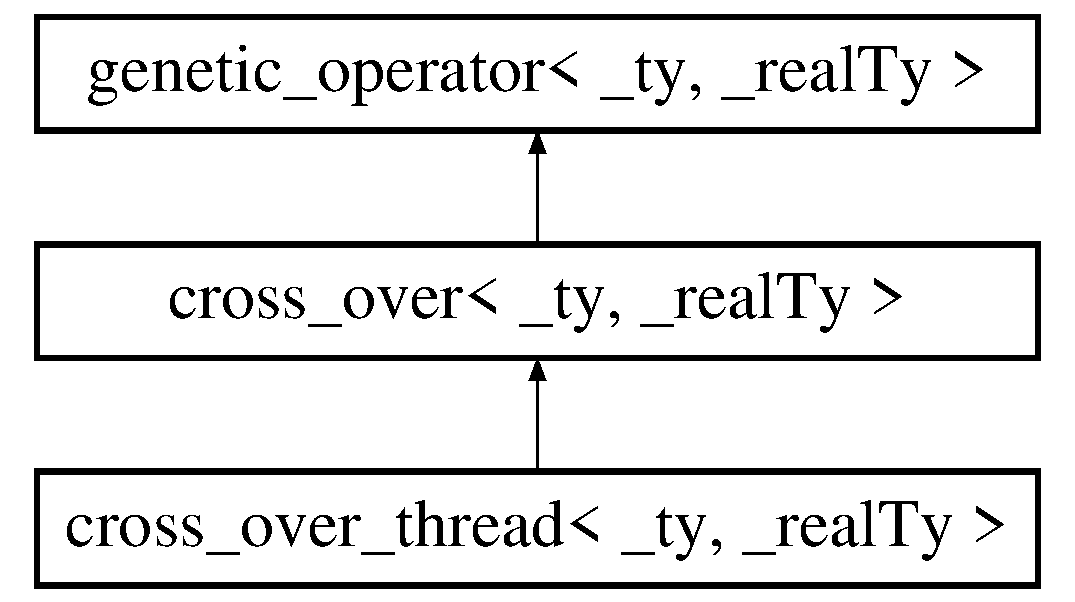
\includegraphics[height=3cm]{classcross__over}
\end{center}
\end{figure}
\subsection*{Métodos Públicos}
\begin{DoxyCompactItemize}
\item 
\hyperlink{classcross__over_aa3561392e40e80aec88cc88aab4f988d}{cross\_\-over} (\hyperlink{classpopulation}{population}$<$ \_\-ty, \_\-realTy $>$ $\ast$\_\-to\_\-apply\_\-operator=NULL, const int \&number\_\-coordinate=def::genetic\_\-operator::cross\_\-over::number\_\-coordinate, const float \&probability=def::genetic\_\-operator::cross\_\-over::probability, const int \&CP=9, const bool \&aleatory=true)
\item 
const bool \& \hyperlink{classcross__over_a62fa09dbf5e970644ea151d78ce8e2eb}{IsAleatory} (void) const 
\item 
void \hyperlink{classcross__over_a69f0a44b51940c67f996e9da5cda250b}{SetAleatory} (const bool \&new\_\-aleatory)
\item 
virtual void \hyperlink{classcross__over_a241401bf77d5c8c465991baa90b1d01b}{MakePairs} (void)
\item 
bool \hyperlink{classcross__over_ace759185adf45d08ece996286c69542f}{CrossOver} (\hyperlink{classcoordinate}{coordinate}$<$ \_\-ty, \_\-realTy $>$ \&c1, \hyperlink{classcoordinate}{coordinate}$<$ \_\-ty, \_\-realTy $>$ \&c2, const int \&CP)
\end{DoxyCompactItemize}
\subsection*{Métodos Protegidos}
\begin{DoxyCompactItemize}
\item 
virtual void \hyperlink{classcross__over_af8d2e8a02552551f3edd692793816de3}{CrossOver} (\_\-ty \&coord\_\-1, \_\-ty \&coord\_\-2, const int \&CP)
\item 
virtual const char \& \hyperlink{classcross__over_a1a840a73fa36cc7f4f7e769f78d73e81}{WalkOnPopulationHook} (\hyperlink{classindividual}{individual}$<$ \_\-ty, \_\-realTy $>$ \&id)
\item 
virtual const char \& \hyperlink{classcross__over_a1febad7c46ec396173e099372d50839e}{WalkOnIndividualHook} (\hyperlink{classcoordinate}{coordinate}$<$ \_\-ty, \_\-realTy $>$ \&coo)
\end{DoxyCompactItemize}


\subsection{Descrição Detalhada}
\subsubsection*{template$<$typename \_\-ty, typename \_\-realTy$>$ class cross\_\-over$<$ \_\-ty, \_\-realTy $>$}

Classe que encapsula um operador genético de cruzamento. Herda os atributos da classe \hyperlink{classgenetic__operator}{genetic\_\-operator}, já que o o operador genético é um tipo de operador. O método principal é o método \hyperlink{classcross__over_ace759185adf45d08ece996286c69542f}{CrossOver()}, que realiza efetivamente o cruzamento entre dois indivíduos.


\begin{DoxyTemplParams}{Template Parameters}
\item[{\em \_\-ty}]\item[{\em \_\-realTy}]\end{DoxyTemplParams}


\subsection{Construtores \& Destrutores}
\hypertarget{classcross__over_aa3561392e40e80aec88cc88aab4f988d}{
\index{cross\_\-over@{cross\_\-over}!cross\_\-over@{cross\_\-over}}
\index{cross\_\-over@{cross\_\-over}!cross_over@{cross\_\-over}}
\subsubsection[{cross\_\-over}]{\setlength{\rightskip}{0pt plus 5cm}template$<$typename \_\-ty , typename \_\-realTy $>$ {\bf cross\_\-over}$<$ \_\-ty, \_\-realTy $>$::{\bf cross\_\-over} ({\bf population}$<$ \_\-ty, \_\-realTy $>$ $\ast$ {\em \_\-to\_\-apply\_\-operator} = {\ttfamily NULL}, \/  const int \& {\em number\_\-coordinate} = {\ttfamily def::genetic\_\-operator::cross\_\-over$<$~\_\-ty,~\_\-realTy~$>$::number\_\-coordinate}, \/  const float \& {\em probability} = {\ttfamily def::genetic\_\-operator::cross\_\-over$<$~\_\-ty,~\_\-realTy~$>$::probability}, \/  const int \& {\em CP} = {\ttfamily 9}, \/  const bool \& {\em aleatory} = {\ttfamily true})\hspace{0.3cm}{\ttfamily  \mbox{[}inline\mbox{]}}}}
\label{classcross__over_aa3561392e40e80aec88cc88aab4f988d}
Método construtor

\_\-to\_\-apply\_\-operator Ponteiro para a população na qual o operador irá realizar o cruzamento.  number\_\-coordinate Búmero de coordenadas das coordeanadas da população.  probability Probabilidade da realazição do cruzamento.  CP Ponto de corte do cruzamento.  aleatory Se o ponto de corte é aleatório ou não. 

\subsection{Métodos}
\hypertarget{classcross__over_af8d2e8a02552551f3edd692793816de3}{
\index{cross\_\-over@{cross\_\-over}!CrossOver@{CrossOver}}
\index{CrossOver@{CrossOver}!cross_over@{cross\_\-over}}
\subsubsection[{CrossOver}]{\setlength{\rightskip}{0pt plus 5cm}template$<$typename \_\-ty , typename \_\-realTy $>$ void {\bf cross\_\-over}$<$ \_\-ty, \_\-realTy $>$::CrossOver (\_\-ty \& {\em coord\_\-1}, \/  \_\-ty \& {\em coord\_\-2}, \/  const int \& {\em CP})\hspace{0.3cm}{\ttfamily  \mbox{[}inline, protected, virtual\mbox{]}}}}
\label{classcross__over_af8d2e8a02552551f3edd692793816de3}
Realiza o cruzamento entre duas coordenadas.

coord\_\-1 Uma das coordenadas que participará do cruzamento.  coord\_\-2 A outra coordenada que participará do cruzamento.  CP O ponto de corte do cruzamento. \hypertarget{classcross__over_ace759185adf45d08ece996286c69542f}{
\index{cross\_\-over@{cross\_\-over}!CrossOver@{CrossOver}}
\index{CrossOver@{CrossOver}!cross_over@{cross\_\-over}}
\subsubsection[{CrossOver}]{\setlength{\rightskip}{0pt plus 5cm}template$<$typename \_\-ty , typename \_\-realTy $>$ bool {\bf cross\_\-over}$<$ \_\-ty, \_\-realTy $>$::CrossOver ({\bf coordinate}$<$ \_\-ty, \_\-realTy $>$ \& {\em c1}, \/  {\bf coordinate}$<$ \_\-ty, \_\-realTy $>$ \& {\em c2}, \/  const int \& {\em CP})\hspace{0.3cm}{\ttfamily  \mbox{[}inline\mbox{]}}}}
\label{classcross__over_ace759185adf45d08ece996286c69542f}
Realiza o cruzamento efetivamente.

c1 Um dos indivíduos do par que poderá ser cruzado.  c2 O outro indivíduo do par que poderá ser cruzado.  CP O ponto de corte do cruzamento.

\begin{DoxyReturn}{Retorna}

\end{DoxyReturn}
\hypertarget{classcross__over_a62fa09dbf5e970644ea151d78ce8e2eb}{
\index{cross\_\-over@{cross\_\-over}!IsAleatory@{IsAleatory}}
\index{IsAleatory@{IsAleatory}!cross_over@{cross\_\-over}}
\subsubsection[{IsAleatory}]{\setlength{\rightskip}{0pt plus 5cm}template$<$typename \_\-ty, typename \_\-realTy$>$ const bool\& {\bf cross\_\-over}$<$ \_\-ty, \_\-realTy $>$::IsAleatory (void) const\hspace{0.3cm}{\ttfamily  \mbox{[}inline\mbox{]}}}}
\label{classcross__over_a62fa09dbf5e970644ea151d78ce8e2eb}
Método de interface (get).

\begin{DoxyReturn}{Retorna}
Retorna se o ponto de corte do operador é aleatório. 
\end{DoxyReturn}
\hypertarget{classcross__over_a241401bf77d5c8c465991baa90b1d01b}{
\index{cross\_\-over@{cross\_\-over}!MakePairs@{MakePairs}}
\index{MakePairs@{MakePairs}!cross_over@{cross\_\-over}}
\subsubsection[{MakePairs}]{\setlength{\rightskip}{0pt plus 5cm}template$<$typename \_\-ty , typename \_\-realTy $>$ void {\bf cross\_\-over}$<$ \_\-ty, \_\-realTy $>$::MakePairs (void)\hspace{0.3cm}{\ttfamily  \mbox{[}inline, virtual\mbox{]}}}}
\label{classcross__over_a241401bf77d5c8c465991baa90b1d01b}
Realiza o casamento dos individuos. \hypertarget{classcross__over_a69f0a44b51940c67f996e9da5cda250b}{
\index{cross\_\-over@{cross\_\-over}!SetAleatory@{SetAleatory}}
\index{SetAleatory@{SetAleatory}!cross_over@{cross\_\-over}}
\subsubsection[{SetAleatory}]{\setlength{\rightskip}{0pt plus 5cm}template$<$typename \_\-ty, typename \_\-realTy$>$ void {\bf cross\_\-over}$<$ \_\-ty, \_\-realTy $>$::SetAleatory (const bool \& {\em new\_\-aleatory})\hspace{0.3cm}{\ttfamily  \mbox{[}inline\mbox{]}}}}
\label{classcross__over_a69f0a44b51940c67f996e9da5cda250b}
Método de interface (set).

new\_\-aleatory Valor que fará com que o ponto de corte do operador seja aleatório ou não. \hypertarget{classcross__over_a1febad7c46ec396173e099372d50839e}{
\index{cross\_\-over@{cross\_\-over}!WalkOnIndividualHook@{WalkOnIndividualHook}}
\index{WalkOnIndividualHook@{WalkOnIndividualHook}!cross_over@{cross\_\-over}}
\subsubsection[{WalkOnIndividualHook}]{\setlength{\rightskip}{0pt plus 5cm}template$<$typename \_\-ty , typename \_\-realTy $>$ const char \& {\bf cross\_\-over}$<$ \_\-ty, \_\-realTy $>$::WalkOnIndividualHook ({\bf coordinate}$<$ \_\-ty, \_\-realTy $>$ \& {\em coo})\hspace{0.3cm}{\ttfamily  \mbox{[}inline, protected, virtual\mbox{]}}}}
\label{classcross__over_a1febad7c46ec396173e099372d50839e}
Método de gancho que caminha no vetor de coordenadas aplicando o operador de cruzamento.

coo Coordenada onde será aplicado o operador genético.

\begin{DoxyReturn}{Retorna}
A direção de caminhada do algoritmo. 
\end{DoxyReturn}


Implementa \hyperlink{classgenetic__operator_a2124d70b28b35d3114eb3e3ffa72baef}{genetic\_\-operator$<$ \_\-ty, \_\-realTy $>$}.

\hypertarget{classcross__over_a1a840a73fa36cc7f4f7e769f78d73e81}{
\index{cross\_\-over@{cross\_\-over}!WalkOnPopulationHook@{WalkOnPopulationHook}}
\index{WalkOnPopulationHook@{WalkOnPopulationHook}!cross_over@{cross\_\-over}}
\subsubsection[{WalkOnPopulationHook}]{\setlength{\rightskip}{0pt plus 5cm}template$<$typename \_\-ty , typename \_\-realTy $>$ const char \& {\bf cross\_\-over}$<$ \_\-ty, \_\-realTy $>$::WalkOnPopulationHook ({\bf individual}$<$ \_\-ty, \_\-realTy $>$ \& {\em id})\hspace{0.3cm}{\ttfamily  \mbox{[}inline, protected, virtual\mbox{]}}}}
\label{classcross__over_a1a840a73fa36cc7f4f7e769f78d73e81}
Método de gancho que caminha no vetor de indivíduos aplicando o operador de cruzamento.

id Indivíduo onde será aplicado o operador de cruzamento.

\begin{DoxyReturn}{Retorna}
Um identificador da nova direção de caminhada 
\end{DoxyReturn}


Implementa \hyperlink{classgenetic__operator_a3405bb5335111bd675d408aa8db052fa}{genetic\_\-operator$<$ \_\-ty, \_\-realTy $>$}.



A documentação para esta classe foi gerada a partir do seguinte arquivo:\begin{DoxyCompactItemize}
\item 
\hyperlink{cross__over_8h}{cross\_\-over.h}\end{DoxyCompactItemize}

\hypertarget{classcross__over__thread}{
\section{Referência da Template de Classe cross\_\-over\_\-thread$<$ \_\-ty, \_\-realTy $>$}
\label{classcross__over__thread}\index{cross\_\-over\_\-thread@{cross\_\-over\_\-thread}}
}
Diagrama de Hierarquia para cross\_\-over\_\-thread$<$ \_\-ty, \_\-realTy $>$:\begin{figure}[H]
\begin{center}
\leavevmode
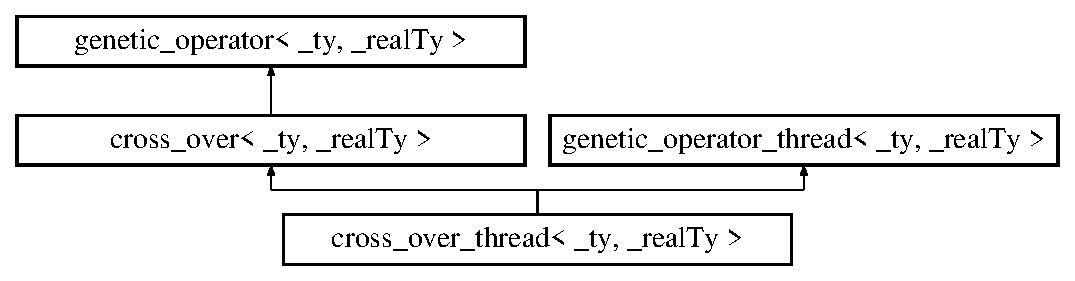
\includegraphics[height=3cm]{classcross__over__thread}
\end{center}
\end{figure}
\subsection*{Métodos Públicos}
\begin{DoxyCompactItemize}
\item 
\hyperlink{classcross__over__thread_acaa709237e2789b033adb64a7217059b}{cross\_\-over\_\-thread} (\hyperlink{classpopulation}{population}$<$ \_\-ty, \_\-realTy $>$ $\ast$popPt)
\item 
\hyperlink{classcross__over__thread_ac0399322791eac4c1e09d1f60653c610}{$\sim$cross\_\-over\_\-thread} ()
\item 
void $\ast$ \hyperlink{classcross__over__thread_a7cc2e9564ebe457e7e7c25d107b5da78}{ConsumeAndProduceIndividuals} (void)
\end{DoxyCompactItemize}
\subsubsection*{template$<$typename \_\-ty, typename \_\-realTy$>$ class cross\_\-over\_\-thread$<$ \_\-ty, \_\-realTy $>$}



\subsection{Construtores \& Destrutores}
\hypertarget{classcross__over__thread_acaa709237e2789b033adb64a7217059b}{
\index{cross\_\-over\_\-thread@{cross\_\-over\_\-thread}!cross\_\-over\_\-thread@{cross\_\-over\_\-thread}}
\index{cross\_\-over\_\-thread@{cross\_\-over\_\-thread}!cross_over_thread@{cross\_\-over\_\-thread}}
\subsubsection[{cross\_\-over\_\-thread}]{\setlength{\rightskip}{0pt plus 5cm}template$<$typename \_\-ty , typename \_\-realTy $>$ {\bf cross\_\-over\_\-thread}$<$ \_\-ty, \_\-realTy $>$::{\bf cross\_\-over\_\-thread} ({\bf population}$<$ \_\-ty, \_\-realTy $>$ $\ast$ {\em popPt})\hspace{0.3cm}{\ttfamily  \mbox{[}inline\mbox{]}}}}
\label{classcross__over__thread_acaa709237e2789b033adb64a7217059b}
Método construtor.

popPt Ponteiro para a população que irá realizar o cruzamento. \hypertarget{classcross__over__thread_ac0399322791eac4c1e09d1f60653c610}{
\index{cross\_\-over\_\-thread@{cross\_\-over\_\-thread}!$\sim$cross\_\-over\_\-thread@{$\sim$cross\_\-over\_\-thread}}
\index{$\sim$cross\_\-over\_\-thread@{$\sim$cross\_\-over\_\-thread}!cross_over_thread@{cross\_\-over\_\-thread}}
\subsubsection[{$\sim$cross\_\-over\_\-thread}]{\setlength{\rightskip}{0pt plus 5cm}template$<$typename \_\-ty, typename \_\-realTy$>$ {\bf cross\_\-over\_\-thread}$<$ \_\-ty, \_\-realTy $>$::$\sim${\bf cross\_\-over\_\-thread} ()}}
\label{classcross__over__thread_ac0399322791eac4c1e09d1f60653c610}
Método destrutor. 

\subsection{Métodos}
\hypertarget{classcross__over__thread_a7cc2e9564ebe457e7e7c25d107b5da78}{
\index{cross\_\-over\_\-thread@{cross\_\-over\_\-thread}!ConsumeAndProduceIndividuals@{ConsumeAndProduceIndividuals}}
\index{ConsumeAndProduceIndividuals@{ConsumeAndProduceIndividuals}!cross_over_thread@{cross\_\-over\_\-thread}}
\subsubsection[{ConsumeAndProduceIndividuals}]{\setlength{\rightskip}{0pt plus 5cm}template$<$typename \_\-ty , typename \_\-realTy $>$ void $\ast$ {\bf cross\_\-over\_\-thread}$<$ \_\-ty, \_\-realTy $>$::ConsumeAndProduceIndividuals (void)\hspace{0.3cm}{\ttfamily  \mbox{[}inline\mbox{]}}}}
\label{classcross__over__thread_a7cc2e9564ebe457e7e7c25d107b5da78}
Métod que realmente executa o cruzamento, ou seja que é executado pelas threads.

\begin{DoxyReturn}{Retorna}
Um ponteiro NULL. 
\end{DoxyReturn}


A documentação para esta classe foi gerada a partir do seguinte arquivo:\begin{DoxyCompactItemize}
\item 
cross\_\-over\_\-thread.h\end{DoxyCompactItemize}

\hypertarget{classga__exception}{
\section{Referência da Classe ga\_\-exception}
\label{classga__exception}\index{ga\_\-exception@{ga\_\-exception}}
}


{\ttfamily \#include $<$ga\_\-exception.h$>$}

\subsection*{Métodos Públicos}
\begin{DoxyCompactItemize}
\item 
\hyperlink{classga__exception_a92dc4bfb0206de9f8a107f2545eb3bb8}{ga\_\-exception} (std::string line, std::string func, std::string file)
\item 
std::string \hyperlink{classga__exception_ab636963c37205d48c5b8f00ef353bed0}{what} (void)
\end{DoxyCompactItemize}


\subsection{Descrição Detalhada}
Classe que trata as excessões do GA. 

\subsection{Construtores \& Destrutores}
\hypertarget{classga__exception_a92dc4bfb0206de9f8a107f2545eb3bb8}{
\index{ga\_\-exception@{ga\_\-exception}!ga\_\-exception@{ga\_\-exception}}
\index{ga\_\-exception@{ga\_\-exception}!ga_exception@{ga\_\-exception}}
\subsubsection[{ga\_\-exception}]{\setlength{\rightskip}{0pt plus 5cm}ga\_\-exception::ga\_\-exception (std::string {\em line}, \/  std::string {\em func}, \/  std::string {\em file})\hspace{0.3cm}{\ttfamily  \mbox{[}inline\mbox{]}}}}
\label{classga__exception_a92dc4bfb0206de9f8a107f2545eb3bb8}
Método construtor da excessão.

line Linha onde ocorreu a excessão.  func Nome do método onde ocorreu a excessão.  file Arquivo aonde ocorreu a excessão. 

\subsection{Métodos}
\hypertarget{classga__exception_ab636963c37205d48c5b8f00ef353bed0}{
\index{ga\_\-exception@{ga\_\-exception}!what@{what}}
\index{what@{what}!ga_exception@{ga\_\-exception}}
\subsubsection[{what}]{\setlength{\rightskip}{0pt plus 5cm}std::string ga\_\-exception::what (void)\hspace{0.3cm}{\ttfamily  \mbox{[}inline\mbox{]}}}}
\label{classga__exception_ab636963c37205d48c5b8f00ef353bed0}
Retorna a descrição detalhada da excessão.

\begin{DoxyReturn}{Retorna}
String com os detalhes da excessão. 
\end{DoxyReturn}


A documentação para esta classe foi gerada a partir do seguinte arquivo:\begin{DoxyCompactItemize}
\item 
\hyperlink{ga__exception_8h}{ga\_\-exception.h}\end{DoxyCompactItemize}

\hypertarget{classgenetic__algorithm}{
\section{Referência da Template de Classe genetic\_\-algorithm$<$ \_\-ty, \_\-realTy $>$}
\label{classgenetic__algorithm}\index{genetic\_\-algorithm@{genetic\_\-algorithm}}
}


{\ttfamily \#include $<$genetic\_\-algorithm.h$>$}

Diagrama de Hierarquia para genetic\_\-algorithm$<$ \_\-ty, \_\-realTy $>$:\begin{figure}[H]
\begin{center}
\leavevmode
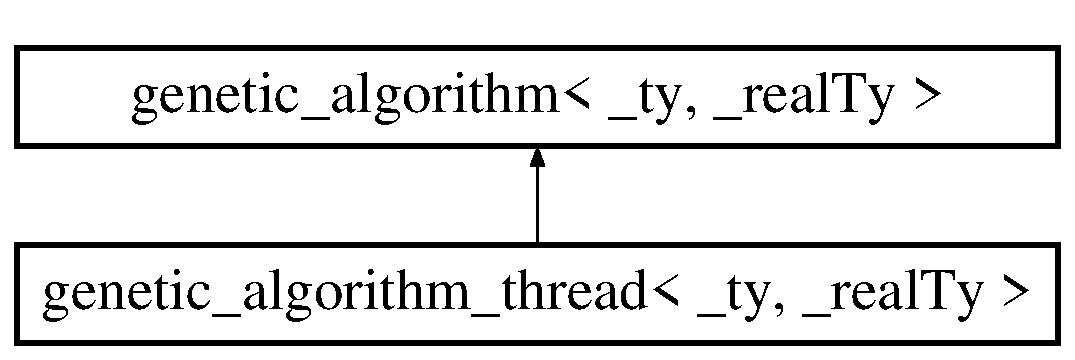
\includegraphics[height=2cm]{classgenetic__algorithm}
\end{center}
\end{figure}
\subsection*{Métodos Públicos}
\begin{DoxyCompactItemize}
\item 
\hyperlink{classgenetic__algorithm_af33b707193eeea4557c46ddb0bde22b6}{genetic\_\-algorithm} (const int \&max\_\-generation=1000)
\item 
const int \& \hyperlink{classgenetic__algorithm_ab125057b9774303bab463defd29000e1}{GetMaxGeneration} (void) const 
\item 
void \hyperlink{classgenetic__algorithm_ad7e8c1a4ce92a617bf2d2a4496a4a31b}{SeMaxGeneration} (const int \&new\_\-max)
\item 
void \hyperlink{classgenetic__algorithm_a9a875d5695bfcc574b616f69e1605427}{StartGA} (void)
\end{DoxyCompactItemize}
\subsection*{Atributos Protegidos}
\begin{DoxyCompactItemize}
\item 
\hyperlink{classpopulation}{population}$<$ \_\-ty, \_\-realTy $>$ $\ast$ \hyperlink{classgenetic__algorithm_a1b2109867086541f375f091a34b1413b}{\_\-population}
\item 
int \hyperlink{classgenetic__algorithm_aa27789d88ad571a15a9ad984f238f51e}{\_\-max\_\-generation}
\item 
\hyperlink{classgenetic__operator}{genetic\_\-operator}$<$\_\-ty, \_\-realTy $>$ $\ast$ \hyperlink{classgenetic__algorithm_a9f03558907645bff987053e1571c9816}{\_\-mutation}
\item 
\hyperlink{classcross__over}{cross\_\-over}$<$ \_\-ty, \_\-realTy $>$ $\ast$ \hyperlink{classgenetic__algorithm_a4b1145baa8b987a6e69681f79a939b24}{\_\-cross\_\-over}
\item 
\hyperlink{classgenetic__operator}{genetic\_\-operator}$<$\_\-ty, \_\-realTy $>$ $\ast$ \hyperlink{classgenetic__algorithm_a237298e9294747b7531beca4df11e049}{\_\-selection}
\end{DoxyCompactItemize}


\subsection{Descrição Detalhada}
\subsubsection*{template$<$typename \_\-ty, typename \_\-realTy$>$ class genetic\_\-algorithm$<$ \_\-ty, \_\-realTy $>$}

Classe que encapsula os conceitos do algoritmo genético e inicia o GA.


\begin{DoxyTemplParams}{Template Parameters}
\item[{\em \_\-ty}]\item[{\em \_\-realTy}]\end{DoxyTemplParams}


\subsection{Construtores \& Destrutores}
\hypertarget{classgenetic__algorithm_af33b707193eeea4557c46ddb0bde22b6}{
\index{genetic\_\-algorithm@{genetic\_\-algorithm}!genetic\_\-algorithm@{genetic\_\-algorithm}}
\index{genetic\_\-algorithm@{genetic\_\-algorithm}!genetic_algorithm@{genetic\_\-algorithm}}
\subsubsection[{genetic\_\-algorithm}]{\setlength{\rightskip}{0pt plus 5cm}template$<$typename \_\-ty , typename \_\-realTy $>$ {\bf genetic\_\-algorithm}$<$ \_\-ty, \_\-realTy $>$::{\bf genetic\_\-algorithm} (const int \& {\em max\_\-generation} = {\ttfamily 1000})\hspace{0.3cm}{\ttfamily  \mbox{[}inline\mbox{]}}}}
\label{classgenetic__algorithm_af33b707193eeea4557c46ddb0bde22b6}
Método construtor

max\_\-generation Número máximo de gerações. 

\subsection{Métodos}
\hypertarget{classgenetic__algorithm_ab125057b9774303bab463defd29000e1}{
\index{genetic\_\-algorithm@{genetic\_\-algorithm}!GetMaxGeneration@{GetMaxGeneration}}
\index{GetMaxGeneration@{GetMaxGeneration}!genetic_algorithm@{genetic\_\-algorithm}}
\subsubsection[{GetMaxGeneration}]{\setlength{\rightskip}{0pt plus 5cm}template$<$typename \_\-ty , typename \_\-realTy $>$ const int\& {\bf genetic\_\-algorithm}$<$ \_\-ty, \_\-realTy $>$::GetMaxGeneration (void) const\hspace{0.3cm}{\ttfamily  \mbox{[}inline\mbox{]}}}}
\label{classgenetic__algorithm_ab125057b9774303bab463defd29000e1}
Método de interface (get).

\begin{DoxyReturn}{Retorna}
O número máximo de gerações. 
\end{DoxyReturn}
\hypertarget{classgenetic__algorithm_ad7e8c1a4ce92a617bf2d2a4496a4a31b}{
\index{genetic\_\-algorithm@{genetic\_\-algorithm}!SeMaxGeneration@{SeMaxGeneration}}
\index{SeMaxGeneration@{SeMaxGeneration}!genetic_algorithm@{genetic\_\-algorithm}}
\subsubsection[{SeMaxGeneration}]{\setlength{\rightskip}{0pt plus 5cm}template$<$typename \_\-ty , typename \_\-realTy $>$ void {\bf genetic\_\-algorithm}$<$ \_\-ty, \_\-realTy $>$::SeMaxGeneration (const int \& {\em new\_\-max})\hspace{0.3cm}{\ttfamily  \mbox{[}inline\mbox{]}}}}
\label{classgenetic__algorithm_ad7e8c1a4ce92a617bf2d2a4496a4a31b}
Método de interface (set).

new\_\-max O novo valor do número máximo de gerações. \hypertarget{classgenetic__algorithm_a9a875d5695bfcc574b616f69e1605427}{
\index{genetic\_\-algorithm@{genetic\_\-algorithm}!StartGA@{StartGA}}
\index{StartGA@{StartGA}!genetic_algorithm@{genetic\_\-algorithm}}
\subsubsection[{StartGA}]{\setlength{\rightskip}{0pt plus 5cm}template$<$typename \_\-ty , typename \_\-realTy $>$ void {\bf genetic\_\-algorithm}$<$ \_\-ty, \_\-realTy $>$::StartGA (void)\hspace{0.3cm}{\ttfamily  \mbox{[}inline\mbox{]}}}}
\label{classgenetic__algorithm_a9a875d5695bfcc574b616f69e1605427}
Método que irá iniciar o algoritmo genético. 

\subsection{Atributos}
\hypertarget{classgenetic__algorithm_a4b1145baa8b987a6e69681f79a939b24}{
\index{genetic\_\-algorithm@{genetic\_\-algorithm}!\_\-cross\_\-over@{\_\-cross\_\-over}}
\index{\_\-cross\_\-over@{\_\-cross\_\-over}!genetic_algorithm@{genetic\_\-algorithm}}
\subsubsection[{\_\-cross\_\-over}]{\setlength{\rightskip}{0pt plus 5cm}template$<$typename \_\-ty , typename \_\-realTy $>$ {\bf cross\_\-over}$<$\_\-ty,\_\-realTy$>$$\ast$ {\bf genetic\_\-algorithm}$<$ \_\-ty, \_\-realTy $>$::{\bf \_\-cross\_\-over}\hspace{0.3cm}{\ttfamily  \mbox{[}protected\mbox{]}}}}
\label{classgenetic__algorithm_a4b1145baa8b987a6e69681f79a939b24}
Operador genético de cruzamento do GA. \hypertarget{classgenetic__algorithm_aa27789d88ad571a15a9ad984f238f51e}{
\index{genetic\_\-algorithm@{genetic\_\-algorithm}!\_\-max\_\-generation@{\_\-max\_\-generation}}
\index{\_\-max\_\-generation@{\_\-max\_\-generation}!genetic_algorithm@{genetic\_\-algorithm}}
\subsubsection[{\_\-max\_\-generation}]{\setlength{\rightskip}{0pt plus 5cm}template$<$typename \_\-ty , typename \_\-realTy $>$ int {\bf genetic\_\-algorithm}$<$ \_\-ty, \_\-realTy $>$::{\bf \_\-max\_\-generation}\hspace{0.3cm}{\ttfamily  \mbox{[}protected\mbox{]}}}}
\label{classgenetic__algorithm_aa27789d88ad571a15a9ad984f238f51e}
Número máximo de gerações do GA. \hypertarget{classgenetic__algorithm_a9f03558907645bff987053e1571c9816}{
\index{genetic\_\-algorithm@{genetic\_\-algorithm}!\_\-mutation@{\_\-mutation}}
\index{\_\-mutation@{\_\-mutation}!genetic_algorithm@{genetic\_\-algorithm}}
\subsubsection[{\_\-mutation}]{\setlength{\rightskip}{0pt plus 5cm}template$<$typename \_\-ty , typename \_\-realTy $>$ {\bf genetic\_\-operator}$<$\_\-ty,\_\-realTy$>$$\ast$ {\bf genetic\_\-algorithm}$<$ \_\-ty, \_\-realTy $>$::{\bf \_\-mutation}\hspace{0.3cm}{\ttfamily  \mbox{[}protected\mbox{]}}}}
\label{classgenetic__algorithm_a9f03558907645bff987053e1571c9816}
Operador genético de mutação do GA. \hypertarget{classgenetic__algorithm_a1b2109867086541f375f091a34b1413b}{
\index{genetic\_\-algorithm@{genetic\_\-algorithm}!\_\-population@{\_\-population}}
\index{\_\-population@{\_\-population}!genetic_algorithm@{genetic\_\-algorithm}}
\subsubsection[{\_\-population}]{\setlength{\rightskip}{0pt plus 5cm}template$<$typename \_\-ty , typename \_\-realTy $>$ {\bf population}$<$\_\-ty,\_\-realTy$>$$\ast$ {\bf genetic\_\-algorithm}$<$ \_\-ty, \_\-realTy $>$::{\bf \_\-population}\hspace{0.3cm}{\ttfamily  \mbox{[}protected\mbox{]}}}}
\label{classgenetic__algorithm_a1b2109867086541f375f091a34b1413b}
População do GA \hypertarget{classgenetic__algorithm_a237298e9294747b7531beca4df11e049}{
\index{genetic\_\-algorithm@{genetic\_\-algorithm}!\_\-selection@{\_\-selection}}
\index{\_\-selection@{\_\-selection}!genetic_algorithm@{genetic\_\-algorithm}}
\subsubsection[{\_\-selection}]{\setlength{\rightskip}{0pt plus 5cm}template$<$typename \_\-ty , typename \_\-realTy $>$ {\bf genetic\_\-operator}$<$\_\-ty,\_\-realTy$>$$\ast$ {\bf genetic\_\-algorithm}$<$ \_\-ty, \_\-realTy $>$::{\bf \_\-selection}\hspace{0.3cm}{\ttfamily  \mbox{[}protected\mbox{]}}}}
\label{classgenetic__algorithm_a237298e9294747b7531beca4df11e049}
Operador genético de seleção do GA. 

A documentação para esta classe foi gerada a partir do seguinte arquivo:\begin{DoxyCompactItemize}
\item 
\hyperlink{genetic__algorithm_8h}{genetic\_\-algorithm.h}\end{DoxyCompactItemize}

\hypertarget{classgenetic__algorithm__thread}{
\section{Referência da Template de Classe genetic\_\-algorithm\_\-thread$<$ \_\-ty, \_\-realTy $>$}
\label{classgenetic__algorithm__thread}\index{genetic\_\-algorithm\_\-thread@{genetic\_\-algorithm\_\-thread}}
}


{\ttfamily \#include $<$genetic\_\-algorithm\_\-thread.h$>$}

Diagrama de Hierarquia para genetic\_\-algorithm\_\-thread$<$ \_\-ty, \_\-realTy $>$:\begin{figure}[H]
\begin{center}
\leavevmode
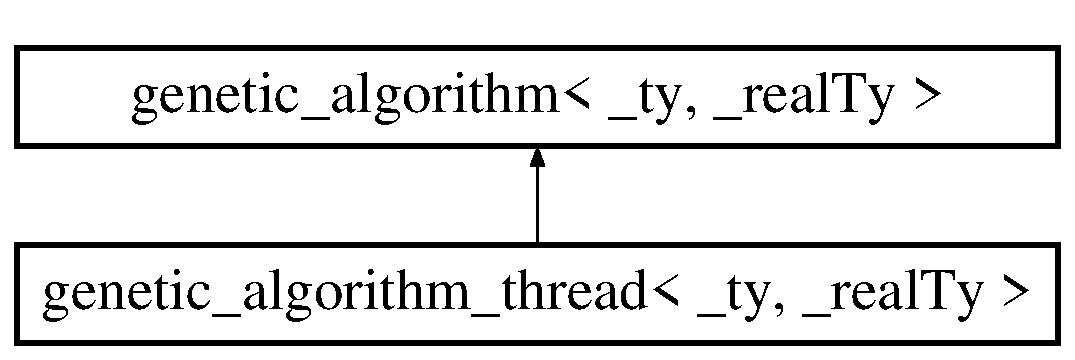
\includegraphics[height=2cm]{classgenetic__algorithm__thread}
\end{center}
\end{figure}
\subsection*{Métodos Públicos}
\begin{DoxyCompactItemize}
\item 
\hyperlink{classgenetic__algorithm__thread_aa09321fa64467ad8dbe34d809eb786da}{genetic\_\-algorithm\_\-thread} (const int \&max\_\-generation)
\end{DoxyCompactItemize}


\subsection{Descrição Detalhada}
\subsubsection*{template$<$typename \_\-ty, typename \_\-realTy$>$ class genetic\_\-algorithm\_\-thread$<$ \_\-ty, \_\-realTy $>$}

Classe que implementa a versão paralelizada do algoritmo genético. Todas as threds são criadas no método construtor, assim como o resultado final do algoritmo.


\begin{DoxyTemplParams}{Template Parameters}
\item[{\em \_\-ty}]\item[{\em \_\-realTy}]\end{DoxyTemplParams}


\subsection{Construtores \& Destrutores}
\hypertarget{classgenetic__algorithm__thread_aa09321fa64467ad8dbe34d809eb786da}{
\index{genetic\_\-algorithm\_\-thread@{genetic\_\-algorithm\_\-thread}!genetic\_\-algorithm\_\-thread@{genetic\_\-algorithm\_\-thread}}
\index{genetic\_\-algorithm\_\-thread@{genetic\_\-algorithm\_\-thread}!genetic_algorithm_thread@{genetic\_\-algorithm\_\-thread}}
\subsubsection[{genetic\_\-algorithm\_\-thread}]{\setlength{\rightskip}{0pt plus 5cm}template$<$typename \_\-ty , typename \_\-realTy $>$ {\bf genetic\_\-algorithm\_\-thread}$<$ \_\-ty, \_\-realTy $>$::{\bf genetic\_\-algorithm\_\-thread} (const int \& {\em max\_\-generation})\hspace{0.3cm}{\ttfamily  \mbox{[}inline\mbox{]}}}}
\label{classgenetic__algorithm__thread_aa09321fa64467ad8dbe34d809eb786da}
Método construtor.

max\_\-generation Número máximo de gerações. 

A documentação para esta classe foi gerada a partir do seguinte arquivo:\begin{DoxyCompactItemize}
\item 
\hyperlink{genetic__algorithm__thread_8h}{genetic\_\-algorithm\_\-thread.h}\end{DoxyCompactItemize}

\hypertarget{classgenetic__operator}{
\section{Referência da Template de Classe genetic\_\-operator$<$ \_\-ty, \_\-realTy $>$}
\label{classgenetic__operator}\index{genetic\_\-operator@{genetic\_\-operator}}
}
Diagrama de Hierarquia para genetic\_\-operator$<$ \_\-ty, \_\-realTy $>$:\begin{figure}[H]
\begin{center}
\leavevmode
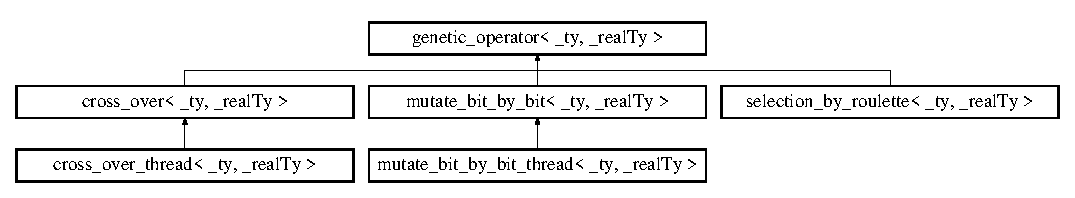
\includegraphics[height=2.21344cm]{classgenetic__operator}
\end{center}
\end{figure}
\subsection*{Métodos Públicos}
\begin{DoxyCompactItemize}
\item 
\hyperlink{classgenetic__operator_a114de57cea1aa2b6db81389ddf5be520}{genetic\_\-operator} (\hyperlink{classpopulation}{population}$<$ \_\-ty, \_\-realTy $>$ $\ast$pt\_\-to\_\-apply\_\-operator=NULL, const float \&probability=def::genetic\_\-operator::probability)
\item 
virtual void \hyperlink{classgenetic__operator_a70569d059114efa73bcd45a264953d13}{doApplyGeneticOperator} (void)
\item 
const \_\-realTy \hyperlink{classgenetic__operator_a406eeb5144dd74698fcd9a120f021aba}{GenerateRandom} (const \_\-realTy \&max=1, const \_\-realTy \&min=0, const int \&precision=def::genetic\_\-operator::precision)
\item 
const \_\-ty \hyperlink{classgenetic__operator_ad9f7ea3ff91063cde8959794b1ac5679}{GenerateRandom} (const \_\-ty \&max, const \_\-ty \&min=0)
\item 
virtual const char \& \hyperlink{classgenetic__operator_a3405bb5335111bd675d408aa8db052fa}{WalkOnPopulationHook} (\hyperlink{classindividual}{individual}$<$ \_\-ty, \_\-realTy $>$ \&id)=0
\item 
virtual const char \& \hyperlink{classgenetic__operator_a2124d70b28b35d3114eb3e3ffa72baef}{WalkOnIndividualHook} (\hyperlink{classcoordinate}{coordinate}$<$ \_\-ty, \_\-realTy $>$ \&coo)=0
\item 
virtual std::string \hyperlink{classgenetic__operator_ae0f79368c0b4ad0cff3f608727bd87f5}{GetName} (void)
\end{DoxyCompactItemize}
\subsection*{Atributos Protegidos}
\begin{DoxyCompactItemize}
\item 
\hypertarget{classgenetic__operator_a5d8f57b5d777bb2ec2f71ab2a21847fc}{
\hyperlink{classpopulation}{population}$<$ \_\-ty, \_\-realTy $>$ $\ast$ {\bfseries \_\-to\_\-apply\_\-operator}}
\label{classgenetic__operator_a5d8f57b5d777bb2ec2f71ab2a21847fc}

\item 
\hypertarget{classgenetic__operator_a8d05857f8efcc48ba94f502b2eb7f277}{
float {\bfseries \_\-probability}}
\label{classgenetic__operator_a8d05857f8efcc48ba94f502b2eb7f277}

\end{DoxyCompactItemize}
\subsubsection*{template$<$typename \_\-ty, typename \_\-realTy$>$ class genetic\_\-operator$<$ \_\-ty, \_\-realTy $>$}



\subsection{Construtores \& Destrutores}
\hypertarget{classgenetic__operator_a114de57cea1aa2b6db81389ddf5be520}{
\index{genetic\_\-operator@{genetic\_\-operator}!genetic\_\-operator@{genetic\_\-operator}}
\index{genetic\_\-operator@{genetic\_\-operator}!genetic_operator@{genetic\_\-operator}}
\subsubsection[{genetic\_\-operator}]{\setlength{\rightskip}{0pt plus 5cm}template$<$typename \_\-ty , typename \_\-realTy $>$ {\bf genetic\_\-operator}$<$ \_\-ty, \_\-realTy $>$::{\bf genetic\_\-operator} ({\bf population}$<$ \_\-ty, \_\-realTy $>$ $\ast$ {\em pt\_\-to\_\-apply\_\-operator} = {\ttfamily NULL}, \/  const float \& {\em probability} = {\ttfamily def::genetic\_\-operator$<$~\_\-ty,~\_\-realTy~$>$::probability})\hspace{0.3cm}{\ttfamily  \mbox{[}inline\mbox{]}}}}
\label{classgenetic__operator_a114de57cea1aa2b6db81389ddf5be520}
Método construtor.

pt\_\-to\_\-apply\_\-operator Ponteiro para o objeto população aonde será aplicado o operador genético.  probability Probabilidade do operador genético realizar uma operação. 

\subsection{Métodos}
\hypertarget{classgenetic__operator_a70569d059114efa73bcd45a264953d13}{
\index{genetic\_\-operator@{genetic\_\-operator}!doApplyGeneticOperator@{doApplyGeneticOperator}}
\index{doApplyGeneticOperator@{doApplyGeneticOperator}!genetic_operator@{genetic\_\-operator}}
\subsubsection[{doApplyGeneticOperator}]{\setlength{\rightskip}{0pt plus 5cm}template$<$typename \_\-ty , typename \_\-realTy $>$ void {\bf genetic\_\-operator}$<$ \_\-ty, \_\-realTy $>$::doApplyGeneticOperator (void)\hspace{0.3cm}{\ttfamily  \mbox{[}inline, virtual\mbox{]}}}}
\label{classgenetic__operator_a70569d059114efa73bcd45a264953d13}
Método virtual que realiza a mutação \hypertarget{classgenetic__operator_ad9f7ea3ff91063cde8959794b1ac5679}{
\index{genetic\_\-operator@{genetic\_\-operator}!GenerateRandom@{GenerateRandom}}
\index{GenerateRandom@{GenerateRandom}!genetic_operator@{genetic\_\-operator}}
\subsubsection[{GenerateRandom}]{\setlength{\rightskip}{0pt plus 5cm}template$<$typename \_\-ty , typename \_\-realTy $>$ const \_\-ty {\bf genetic\_\-operator}$<$ \_\-ty, \_\-realTy $>$::GenerateRandom (const \_\-ty \& {\em max}, \/  const \_\-ty \& {\em min} = {\ttfamily 0})\hspace{0.3cm}{\ttfamily  \mbox{[}inline\mbox{]}}}}
\label{classgenetic__operator_ad9f7ea3ff91063cde8959794b1ac5679}
Método que retorna um número entre min e max do tipo \_\-ty(sem ponto flutuante)

max Valor máximo do intervalo do número aleatório a ser gerado.  min Valor mínimo do intervalo do número aleatório a ser gerado.

\begin{DoxyReturn}{Retorna}
Um número aleatório entre os valores min e max. 
\end{DoxyReturn}
\hypertarget{classgenetic__operator_a406eeb5144dd74698fcd9a120f021aba}{
\index{genetic\_\-operator@{genetic\_\-operator}!GenerateRandom@{GenerateRandom}}
\index{GenerateRandom@{GenerateRandom}!genetic_operator@{genetic\_\-operator}}
\subsubsection[{GenerateRandom}]{\setlength{\rightskip}{0pt plus 5cm}template$<$typename \_\-ty , typename \_\-realTy $>$ const \_\-realTy {\bf genetic\_\-operator}$<$ \_\-ty, \_\-realTy $>$::GenerateRandom (const \_\-realTy \& {\em max} = {\ttfamily 1}, \/  const \_\-realTy \& {\em min} = {\ttfamily 0}, \/  const int \& {\em precision} = {\ttfamily def::genetic\_\-operator$<$~\_\-ty,~\_\-realTy~$>$::precision})\hspace{0.3cm}{\ttfamily  \mbox{[}inline\mbox{]}}}}
\label{classgenetic__operator_a406eeb5144dd74698fcd9a120f021aba}
Método que retorna um número aleatório entre min e max do tipo \_\-realTy(ponto flutuante) com precisão de precision casas decimais

max Valor máximo do intervalo do número aleatório a ser gerado.  min Valor mínimo do intervalo do número aleatório a ser gerado.  precision Número de casas decimais do número aleatório gerado.

\begin{DoxyReturn}{Retorna}
Um número aleatório com precision casas decimais e entre os valores min e max. 
\end{DoxyReturn}
\hypertarget{classgenetic__operator_ae0f79368c0b4ad0cff3f608727bd87f5}{
\index{genetic\_\-operator@{genetic\_\-operator}!GetName@{GetName}}
\index{GetName@{GetName}!genetic_operator@{genetic\_\-operator}}
\subsubsection[{GetName}]{\setlength{\rightskip}{0pt plus 5cm}template$<$typename \_\-ty , typename \_\-realTy $>$ virtual std::string {\bf genetic\_\-operator}$<$ \_\-ty, \_\-realTy $>$::GetName (void)\hspace{0.3cm}{\ttfamily  \mbox{[}inline, virtual\mbox{]}}}}
\label{classgenetic__operator_ae0f79368c0b4ad0cff3f608727bd87f5}
Método que retorna o nome da classe, usado no padrão AbstractFactory

\begin{DoxyReturn}{Retorna}
Uma string com o nome do operador. 
\end{DoxyReturn}


Reimplementado por \hyperlink{classmutate__bit__by__bit_abdab6da2a2b180f14d71f35c895313a4}{mutate\_\-bit\_\-by\_\-bit$<$ \_\-ty, \_\-realTy $>$} e \hyperlink{classselection__by__roulette_a137f1a757ab4d71a0ca0bdba7f9f35d0}{selection\_\-by\_\-roulette$<$ \_\-ty, \_\-realTy $>$}.

\hypertarget{classgenetic__operator_a2124d70b28b35d3114eb3e3ffa72baef}{
\index{genetic\_\-operator@{genetic\_\-operator}!WalkOnIndividualHook@{WalkOnIndividualHook}}
\index{WalkOnIndividualHook@{WalkOnIndividualHook}!genetic_operator@{genetic\_\-operator}}
\subsubsection[{WalkOnIndividualHook}]{\setlength{\rightskip}{0pt plus 5cm}template$<$typename \_\-ty , typename \_\-realTy $>$ virtual const char\& {\bf genetic\_\-operator}$<$ \_\-ty, \_\-realTy $>$::WalkOnIndividualHook ({\bf coordinate}$<$ \_\-ty, \_\-realTy $>$ \& {\em coo})\hspace{0.3cm}{\ttfamily  \mbox{[}pure virtual\mbox{]}}}}
\label{classgenetic__operator_a2124d70b28b35d3114eb3e3ffa72baef}
Método de gancho puramente virtual para as classes filhas, usadas no padrão Template Method. Caminha sobre o conteiner de coordenadas do indivíduo, e aplica o operador nas coordenadas.

coo A coordenada onde será aplicado o operador.

\begin{DoxyReturn}{Retorna}
A direção da caminhada nos conteiners. 
\end{DoxyReturn}


Implementado por \hyperlink{classcross__over_a1febad7c46ec396173e099372d50839e}{cross\_\-over$<$ \_\-ty, \_\-realTy $>$}, \hyperlink{classmutate__bit__by__bit_a150b01e7ee79683012f7d60e8c1b9ccc}{mutate\_\-bit\_\-by\_\-bit$<$ \_\-ty, \_\-realTy $>$} e \hyperlink{classselection__by__roulette_abb536fd7b63a452a2ebd8e7572bfc4d8}{selection\_\-by\_\-roulette$<$ \_\-ty, \_\-realTy $>$}.

\hypertarget{classgenetic__operator_a3405bb5335111bd675d408aa8db052fa}{
\index{genetic\_\-operator@{genetic\_\-operator}!WalkOnPopulationHook@{WalkOnPopulationHook}}
\index{WalkOnPopulationHook@{WalkOnPopulationHook}!genetic_operator@{genetic\_\-operator}}
\subsubsection[{WalkOnPopulationHook}]{\setlength{\rightskip}{0pt plus 5cm}template$<$typename \_\-ty , typename \_\-realTy $>$ virtual const char\& {\bf genetic\_\-operator}$<$ \_\-ty, \_\-realTy $>$::WalkOnPopulationHook ({\bf individual}$<$ \_\-ty, \_\-realTy $>$ \& {\em id})\hspace{0.3cm}{\ttfamily  \mbox{[}pure virtual\mbox{]}}}}
\label{classgenetic__operator_a3405bb5335111bd675d408aa8db052fa}
Método de gancho puramente virtual para as classes filhas, usadas no padrão Template Method. Caminha sobre o conteiner de indivíduos da populacao, e aplica o operador nos indivíduos

id Indivíduo em que será aplicado o operador genético.

\begin{DoxyReturn}{Retorna}
A direção da caminhada nos containers. 
\end{DoxyReturn}


Implementado por \hyperlink{classcross__over_a1a840a73fa36cc7f4f7e769f78d73e81}{cross\_\-over$<$ \_\-ty, \_\-realTy $>$}, \hyperlink{classmutate__bit__by__bit_a2f8cc52a35943854f24b7534ecd90c7b}{mutate\_\-bit\_\-by\_\-bit$<$ \_\-ty, \_\-realTy $>$} e \hyperlink{classselection__by__roulette_a98be3d54afb87450f190615f7da330e9}{selection\_\-by\_\-roulette$<$ \_\-ty, \_\-realTy $>$}.



A documentação para esta classe foi gerada a partir do seguinte arquivo:\begin{DoxyCompactItemize}
\item 
\hyperlink{genetic__operator_8h}{genetic\_\-operator.h}\end{DoxyCompactItemize}

\hypertarget{classgenetic__operator__thread}{
\section{Referência da Template de Classe genetic\_\-operator\_\-thread$<$ \_\-ty, \_\-realTy $>$}
\label{classgenetic__operator__thread}\index{genetic\_\-operator\_\-thread@{genetic\_\-operator\_\-thread}}
}


{\ttfamily \#include $<$genetic\_\-operator\_\-thread.h$>$}

Diagrama de Hierarquia para genetic\_\-operator\_\-thread$<$ \_\-ty, \_\-realTy $>$:\begin{figure}[H]
\begin{center}
\leavevmode
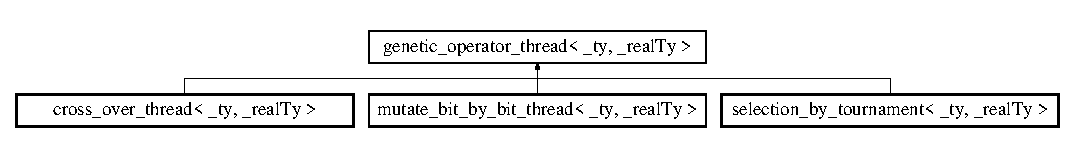
\includegraphics[height=1.47563cm]{classgenetic__operator__thread}
\end{center}
\end{figure}
\subsection*{Tipos Públicos}
\begin{DoxyCompactItemize}
\item 
typedef boost::mutex::scoped\_\-lock \hyperlink{classgenetic__operator__thread_abe926f8fc2a1548516dad216a1acd4fb}{scoped\_\-lock}
\item 
typedef std::vector$<$ boost::thread $\ast$ $>$::iterator \hyperlink{classgenetic__operator__thread_ac5a153e12dd6711746126c48edba271a}{it\_\-}
\end{DoxyCompactItemize}
\subsection*{Métodos Públicos}
\begin{DoxyCompactItemize}
\item 
\hyperlink{classgenetic__operator__thread_a2b60b46c5d55135436590f6aa2b11da3}{genetic\_\-operator\_\-thread} (\hyperlink{classpopulation}{population}$<$$>$ $\ast$popPt)
\item 
\hyperlink{classgenetic__operator__thread_a30c4b7a10dae2ff72905416953a64049}{$\sim$genetic\_\-operator\_\-thread} ()
\item 
\hyperlink{classgenetic__operator__thread_adb72da6103f5995bd4c265789e5eceac}{genetic\_\-operator\_\-thread} (const \hyperlink{classgenetic__operator__thread}{genetic\_\-operator\_\-thread}$<$ \_\-ty, \_\-realTy $>$ \&got)
\item 
\hyperlink{classgenetic__operator__thread}{genetic\_\-operator\_\-thread} $\ast$ \hyperlink{classgenetic__operator__thread_a751c7f678d7486bee8b1a02bb9e60416}{GetReference} (void)
\item 
void \hyperlink{classgenetic__operator__thread_a435435aa8c4e9f50b041b40c7f63b599}{SetProducer} (\hyperlink{classgenetic__operator__thread}{genetic\_\-operator\_\-thread}$<$ \_\-ty, \_\-realTy $>$ $\ast$new\_\-prod\_\-pt)
\item 
void \hyperlink{classgenetic__operator__thread_a2944e0158bc914db042fdcf22a4a4e70}{SetConsumer} (\hyperlink{classgenetic__operator__thread}{genetic\_\-operator\_\-thread} $\ast$cons\_\-pt)
\item 
\hyperlink{classsemaphore}{semaphore} $\ast$ \hyperlink{classgenetic__operator__thread_aa9a6e0370bfd3afe316af822832a8013}{GetSemProducer} (void)
\item 
\hyperlink{classsemaphore}{semaphore} $\ast$ \hyperlink{classgenetic__operator__thread_a73424d811348f5a911da3744dfc08762}{GetSemConsumer} (void)
\item 
void \hyperlink{classgenetic__operator__thread_abd1a0cb47d379e74f3e738f5c75fe7b7}{ApplyGeneticOperator} (void)
\item 
void \hyperlink{classgenetic__operator__thread_a5e739f35ac03b42311540dbf4db25d2e}{AddIndividual} (\hyperlink{classindividual}{individual}$<$ \_\-ty, \_\-realTy $>$ $\ast$newId)
\item 
void \hyperlink{classgenetic__operator__thread_a1e355fe496238b6433bbf9f3f70bf6ad}{PushBackIndividual} (\hyperlink{classindividual}{individual}$<$ \_\-ty, \_\-realTy $>$ $\ast$newId)
\item 
\hyperlink{classindividual}{individual}$<$ \_\-ty, \_\-realTy $>$ $\ast$ \hyperlink{classgenetic__operator__thread_aba37d3926c0ae0f61846a3e98cfeaf39}{GetBestIndividual} (void)
\item 
void \hyperlink{classgenetic__operator__thread_a44556f084005e19742891fae2e3c8df3}{UpdatePopulation} (void)
\item 
void \hyperlink{classgenetic__operator__thread_afaab02a61f5f0a52b37c4f8bda8df131}{PrintPopulation} (void)
\item 
boost::condition \& \hyperlink{classgenetic__operator__thread_adbc04b2ec67ef127c316efd2bfb407c4}{GetCondApplyOp} (void)
\item 
boost::mutex \hyperlink{classgenetic__operator__thread_a0973b32bc54f444ca7afcdcdfef9a38a}{GetMutexCondApplyOp} (void)
\item 
bool \hyperlink{classgenetic__operator__thread_a2fdf96fda297cef206de86300ab7df0c}{FullPopulation} (void) const 
\item 
\hyperlink{classgenetic__operator__thread_ac5a153e12dd6711746126c48edba271a}{it\_\-} \hyperlink{classgenetic__operator__thread_a3f9defee5440ebe6d973bcc8806d64ee}{Begin} (void)
\item 
\hyperlink{classgenetic__operator__thread_ac5a153e12dd6711746126c48edba271a}{it\_\-} \hyperlink{classgenetic__operator__thread_ae836d401cde0a8ac21025348b9fcedf6}{End} (void)
\item 
virtual void \hyperlink{classgenetic__operator__thread_a7c86cee81334320d496fb196920fcc10}{ReadyToReceive} (void)
\end{DoxyCompactItemize}
\subsection*{Métodos Protegidos}
\begin{DoxyCompactItemize}
\item 
\hypertarget{classgenetic__operator__thread_a838af3900b85dfba3b5daa7c9dd1b51c}{
boost::mutex {\bfseries GetInMutex} (void)}
\label{classgenetic__operator__thread_a838af3900b85dfba3b5daa7c9dd1b51c}

\item 
\hypertarget{classgenetic__operator__thread_a83fa2b4627e313d4e28ab946e7673017}{
boost::mutex {\bfseries GetOutMutex} (void)}
\label{classgenetic__operator__thread_a83fa2b4627e313d4e28ab946e7673017}

\item 
void \hyperlink{classgenetic__operator__thread_a856af75479279710968a1aa2b26400de}{IncrementIterator} (typename \hyperlink{classpopulation}{population}$<$ \_\-ty, \_\-realTy $>$::\hyperlink{classgenetic__operator__thread_ac5a153e12dd6711746126c48edba271a}{it\_\-} \&it)
\end{DoxyCompactItemize}
\subsection*{Métodos Protegidos Estáticos}
\begin{DoxyCompactItemize}
\item 
static int \& \hyperlink{classgenetic__operator__thread_a22db2979e50888a982e4d78a874b0193}{GetGenerationCount} (void)
\item 
static void \hyperlink{classgenetic__operator__thread_a77fb097a6fa283eebe5cf6af08dd2cfc}{IncrementGenerationCount} (void)
\item 
static bool \hyperlink{classgenetic__operator__thread_aad1cfa9857458b80ca2f5ba2fa3c5d74}{EndOfGA} (void)
\end{DoxyCompactItemize}
\subsection*{Atributos Protegidos}
\begin{DoxyCompactItemize}
\item 
\hyperlink{classpopulation}{population}$<$ \_\-ty, \_\-realTy $>$ $\ast$ \hyperlink{classgenetic__operator__thread_ae0bb1f4c8c30c5557eefc870d2767d66}{\_\-popOperatorPt}
\item 
\hyperlink{classgenetic__operator__thread}{genetic\_\-operator\_\-thread}$<$ \_\-ty, \_\-realTy $>$ $\ast$ \hyperlink{classgenetic__operator__thread_ad88e4f6c5afb05bbc55d5f44bce88ba2}{\_\-consumidorPt}
\item 
\hyperlink{classgenetic__operator__thread}{genetic\_\-operator\_\-thread}$<$ \_\-ty, \_\-realTy $>$ $\ast$ \hyperlink{classgenetic__operator__thread_af325a8a1c9964fc0eac9e2eeda670499}{\_\-producerPt}
\item 
int \hyperlink{classgenetic__operator__thread_a886d986c24ceb36bff5a77bf58447be0}{\_\-coreNumbers}
\item 
\hypertarget{classgenetic__operator__thread_a33d19c478eee6deee0a1fcb43272cc92}{
\hyperlink{classpopulation}{population}$<$ \_\-ty, \_\-realTy $>$::\hyperlink{classgenetic__operator__thread_ac5a153e12dd6711746126c48edba271a}{it\_\-} {\bfseries \_\-inIterator}}
\label{classgenetic__operator__thread_a33d19c478eee6deee0a1fcb43272cc92}

\item 
\hypertarget{classgenetic__operator__thread_ac403a8cd7cd497e8d98bdd40f417771c}{
boost::mutex {\bfseries \_\-inMutex}}
\label{classgenetic__operator__thread_ac403a8cd7cd497e8d98bdd40f417771c}

\item 
\hypertarget{classgenetic__operator__thread_a11bd7c84a7feb28bfed6e1ea52964fd1}{
\hyperlink{classpopulation}{population}$<$ \_\-ty, \_\-realTy $>$::\hyperlink{classgenetic__operator__thread_ac5a153e12dd6711746126c48edba271a}{it\_\-} {\bfseries \_\-outIterator}}
\label{classgenetic__operator__thread_a11bd7c84a7feb28bfed6e1ea52964fd1}

\item 
\hypertarget{classgenetic__operator__thread_a923a2cd5dfdd1478677f5a05f5dd4063}{
boost::mutex {\bfseries \_\-outMutex}}
\label{classgenetic__operator__thread_a923a2cd5dfdd1478677f5a05f5dd4063}

\item 
\hypertarget{classgenetic__operator__thread_a8e9f788e9d5e9c0ee96de0505525196c}{
\hyperlink{classsemaphore}{semaphore} $\ast$ {\bfseries \_\-semConsumer}}
\label{classgenetic__operator__thread_a8e9f788e9d5e9c0ee96de0505525196c}

\item 
\hypertarget{classgenetic__operator__thread_ae9a9af2ff152c15152f42de2c02be1e3}{
\hyperlink{classsemaphore}{semaphore} $\ast$ {\bfseries \_\-semProducer}}
\label{classgenetic__operator__thread_ae9a9af2ff152c15152f42de2c02be1e3}

\item 
\hypertarget{classgenetic__operator__thread_ab1bee0ae612b0f61b9f2bb15b431ea26}{
boost::condition {\bfseries \_\-condApplyOperator}}
\label{classgenetic__operator__thread_ab1bee0ae612b0f61b9f2bb15b431ea26}

\item 
\hypertarget{classgenetic__operator__thread_a9fd8a736c036bb91234a54db69418464}{
boost::mutex {\bfseries \_\-mutexCondApplyOp}}
\label{classgenetic__operator__thread_a9fd8a736c036bb91234a54db69418464}

\item 
\hypertarget{classgenetic__operator__thread_ac45e4d73d9023af4c7998355b4302f28}{
boost::condition {\bfseries \_\-condStopCondition}}
\label{classgenetic__operator__thread_ac45e4d73d9023af4c7998355b4302f28}

\item 
\hypertarget{classgenetic__operator__thread_aa828c4d595704dcd561e1eec098e3ab3}{
boost::mutex {\bfseries \_\-mutexCondStopCond}}
\label{classgenetic__operator__thread_aa828c4d595704dcd561e1eec098e3ab3}

\item 
\hypertarget{classgenetic__operator__thread_a8007f81975ddd3911ef63682cabcd990}{
std::vector$<$ boost::thread $\ast$ $>$ {\bfseries \_\-threadVec}}
\label{classgenetic__operator__thread_a8007f81975ddd3911ef63682cabcd990}

\end{DoxyCompactItemize}
\subsection*{Atributos Estáticos Protegidos}
\begin{DoxyCompactItemize}
\item 
static int \hyperlink{classgenetic__operator__thread_acdf9606e26ae1240cd1c9fced36c656a}{\_\-genCount} = 0
\item 
static boost::mutex \hyperlink{classgenetic__operator__thread_afb4be1bcb256082a4d6e90faba3e5567}{\_\-MutexgenCount}
\end{DoxyCompactItemize}


\subsection{Descrição Detalhada}
\subsubsection*{template$<$typename \_\-ty, typename \_\-realTy$>$ class genetic\_\-operator\_\-thread$<$ \_\-ty, \_\-realTy $>$}

Classe que possui a definição básica de um operador genético paralelizado.


\begin{DoxyTemplParams}{Template Parameters}
\item[{\em \_\-ty}]\item[{\em \_\-realTy}]\end{DoxyTemplParams}


\subsection{Definições de Tipos}
\hypertarget{classgenetic__operator__thread_ac5a153e12dd6711746126c48edba271a}{
\index{genetic\_\-operator\_\-thread@{genetic\_\-operator\_\-thread}!it\_\-@{it\_\-}}
\index{it\_\-@{it\_\-}!genetic_operator_thread@{genetic\_\-operator\_\-thread}}
\subsubsection[{it\_\-}]{\setlength{\rightskip}{0pt plus 5cm}template$<$typename \_\-ty, typename \_\-realTy$>$ typedef std::vector$<$boost::thread$\ast$$>$::iterator {\bf genetic\_\-operator\_\-thread}$<$ \_\-ty, \_\-realTy $>$::{\bf it\_\-}}}
\label{classgenetic__operator__thread_ac5a153e12dd6711746126c48edba271a}
Iterator para percorrer o vetor de threads. \hypertarget{classgenetic__operator__thread_abe926f8fc2a1548516dad216a1acd4fb}{
\index{genetic\_\-operator\_\-thread@{genetic\_\-operator\_\-thread}!scoped\_\-lock@{scoped\_\-lock}}
\index{scoped\_\-lock@{scoped\_\-lock}!genetic_operator_thread@{genetic\_\-operator\_\-thread}}
\subsubsection[{scoped\_\-lock}]{\setlength{\rightskip}{0pt plus 5cm}template$<$typename \_\-ty, typename \_\-realTy$>$ typedef boost::mutex::scoped\_\-lock {\bf genetic\_\-operator\_\-thread}$<$ \_\-ty, \_\-realTy $>$::{\bf scoped\_\-lock}}}
\label{classgenetic__operator__thread_abe926f8fc2a1548516dad216a1acd4fb}
Definição do padrão scoped lock. 

Reimplementado por \hyperlink{classmutate__bit__by__bit__thread_a059838b054d4de64b20d33d1db7e89c0}{mutate\_\-bit\_\-by\_\-bit\_\-thread$<$ \_\-ty, \_\-realTy $>$} e \hyperlink{classselection__by__tournament_a0ba2a47db6a59696b51f19341719c3fd}{selection\_\-by\_\-tournament$<$ \_\-ty, \_\-realTy $>$}.



\subsection{Construtores \& Destrutores}
\hypertarget{classgenetic__operator__thread_a2b60b46c5d55135436590f6aa2b11da3}{
\index{genetic\_\-operator\_\-thread@{genetic\_\-operator\_\-thread}!genetic\_\-operator\_\-thread@{genetic\_\-operator\_\-thread}}
\index{genetic\_\-operator\_\-thread@{genetic\_\-operator\_\-thread}!genetic_operator_thread@{genetic\_\-operator\_\-thread}}
\subsubsection[{genetic\_\-operator\_\-thread}]{\setlength{\rightskip}{0pt plus 5cm}template$<$typename \_\-ty , typename \_\-realTy $>$ {\bf genetic\_\-operator\_\-thread}$<$ \_\-ty, \_\-realTy $>$::{\bf genetic\_\-operator\_\-thread} ({\bf population}$<$$>$ $\ast$ {\em popPt})\hspace{0.3cm}{\ttfamily  \mbox{[}inline\mbox{]}}}}
\label{classgenetic__operator__thread_a2b60b46c5d55135436590f6aa2b11da3}
Método construtor.

popPt Ponteiro para a população em que se vai aplicar o operador. \hypertarget{classgenetic__operator__thread_adb72da6103f5995bd4c265789e5eceac}{
\index{genetic\_\-operator\_\-thread@{genetic\_\-operator\_\-thread}!genetic\_\-operator\_\-thread@{genetic\_\-operator\_\-thread}}
\index{genetic\_\-operator\_\-thread@{genetic\_\-operator\_\-thread}!genetic_operator_thread@{genetic\_\-operator\_\-thread}}
\subsubsection[{genetic\_\-operator\_\-thread}]{\setlength{\rightskip}{0pt plus 5cm}template$<$typename \_\-ty , typename \_\-realTy $>$ {\bf genetic\_\-operator\_\-thread}$<$ \_\-ty, \_\-realTy $>$::{\bf genetic\_\-operator\_\-thread} (const {\bf genetic\_\-operator\_\-thread}$<$ \_\-ty, \_\-realTy $>$ \& {\em got})\hspace{0.3cm}{\ttfamily  \mbox{[}inline\mbox{]}}}}
\label{classgenetic__operator__thread_adb72da6103f5995bd4c265789e5eceac}
Construtor de cópia.

got Operador genético a ser copiado. 

\subsection{Métodos}
\hypertarget{classgenetic__operator__thread_a5e739f35ac03b42311540dbf4db25d2e}{
\index{genetic\_\-operator\_\-thread@{genetic\_\-operator\_\-thread}!AddIndividual@{AddIndividual}}
\index{AddIndividual@{AddIndividual}!genetic_operator_thread@{genetic\_\-operator\_\-thread}}
\subsubsection[{AddIndividual}]{\setlength{\rightskip}{0pt plus 5cm}template$<$typename \_\-ty , typename \_\-realTy $>$ void {\bf genetic\_\-operator\_\-thread}$<$ \_\-ty, \_\-realTy $>$::AddIndividual ({\bf individual}$<$ \_\-ty, \_\-realTy $>$ $\ast$ {\em newId})\hspace{0.3cm}{\ttfamily  \mbox{[}inline\mbox{]}}}}
\label{classgenetic__operator__thread_a5e739f35ac03b42311540dbf4db25d2e}
Método que adiciona um novo indivíduo ao vetor de indivíduos do operador

newId Ponteiro para o novo indivíduo a ser adicionado \hypertarget{classgenetic__operator__thread_abd1a0cb47d379e74f3e738f5c75fe7b7}{
\index{genetic\_\-operator\_\-thread@{genetic\_\-operator\_\-thread}!ApplyGeneticOperator@{ApplyGeneticOperator}}
\index{ApplyGeneticOperator@{ApplyGeneticOperator}!genetic_operator_thread@{genetic\_\-operator\_\-thread}}
\subsubsection[{ApplyGeneticOperator}]{\setlength{\rightskip}{0pt plus 5cm}template$<$typename \_\-ty , typename \_\-realTy $>$ void {\bf genetic\_\-operator\_\-thread}$<$ \_\-ty, \_\-realTy $>$::ApplyGeneticOperator (void)\hspace{0.3cm}{\ttfamily  \mbox{[}inline\mbox{]}}}}
\label{classgenetic__operator__thread_abd1a0cb47d379e74f3e738f5c75fe7b7}
Método que dispara as threads que aplicam o operador genético \hypertarget{classgenetic__operator__thread_a3f9defee5440ebe6d973bcc8806d64ee}{
\index{genetic\_\-operator\_\-thread@{genetic\_\-operator\_\-thread}!Begin@{Begin}}
\index{Begin@{Begin}!genetic_operator_thread@{genetic\_\-operator\_\-thread}}
\subsubsection[{Begin}]{\setlength{\rightskip}{0pt plus 5cm}template$<$typename \_\-ty, typename \_\-realTy$>$ {\bf it\_\-} {\bf genetic\_\-operator\_\-thread}$<$ \_\-ty, \_\-realTy $>$::Begin (void)\hspace{0.3cm}{\ttfamily  \mbox{[}inline\mbox{]}}}}
\label{classgenetic__operator__thread_a3f9defee5440ebe6d973bcc8806d64ee}
Retorna um iterator para o começo do vetor de threads

\begin{DoxyReturn}{Retorna}
Um iterator para o começo do vetor de threads. 
\end{DoxyReturn}
\hypertarget{classgenetic__operator__thread_ae836d401cde0a8ac21025348b9fcedf6}{
\index{genetic\_\-operator\_\-thread@{genetic\_\-operator\_\-thread}!End@{End}}
\index{End@{End}!genetic_operator_thread@{genetic\_\-operator\_\-thread}}
\subsubsection[{End}]{\setlength{\rightskip}{0pt plus 5cm}template$<$typename \_\-ty, typename \_\-realTy$>$ {\bf it\_\-} {\bf genetic\_\-operator\_\-thread}$<$ \_\-ty, \_\-realTy $>$::End (void)\hspace{0.3cm}{\ttfamily  \mbox{[}inline\mbox{]}}}}
\label{classgenetic__operator__thread_ae836d401cde0a8ac21025348b9fcedf6}
Retorna um iterator para o fim do vetor de threads

\begin{DoxyReturn}{Retorna}
Um iterator para o fim do vetor de threads. 
\end{DoxyReturn}
\hypertarget{classgenetic__operator__thread_aad1cfa9857458b80ca2f5ba2fa3c5d74}{
\index{genetic\_\-operator\_\-thread@{genetic\_\-operator\_\-thread}!EndOfGA@{EndOfGA}}
\index{EndOfGA@{EndOfGA}!genetic_operator_thread@{genetic\_\-operator\_\-thread}}
\subsubsection[{EndOfGA}]{\setlength{\rightskip}{0pt plus 5cm}template$<$typename \_\-ty, typename \_\-realTy$>$ static bool {\bf genetic\_\-operator\_\-thread}$<$ \_\-ty, \_\-realTy $>$::EndOfGA (void)\hspace{0.3cm}{\ttfamily  \mbox{[}inline, static, protected\mbox{]}}}}
\label{classgenetic__operator__thread_aad1cfa9857458b80ca2f5ba2fa3c5d74}
Retorna se o número de gerações chegou ao máximo, ou seja se o algoritmo já terminou.

\begin{DoxyReturn}{Retorna}
True caso o número de gerações já chegou ao máximo, false caso contrário. 
\end{DoxyReturn}
\hypertarget{classgenetic__operator__thread_a2fdf96fda297cef206de86300ab7df0c}{
\index{genetic\_\-operator\_\-thread@{genetic\_\-operator\_\-thread}!FullPopulation@{FullPopulation}}
\index{FullPopulation@{FullPopulation}!genetic_operator_thread@{genetic\_\-operator\_\-thread}}
\subsubsection[{FullPopulation}]{\setlength{\rightskip}{0pt plus 5cm}template$<$typename \_\-ty, typename \_\-realTy$>$ bool {\bf genetic\_\-operator\_\-thread}$<$ \_\-ty, \_\-realTy $>$::FullPopulation (void) const\hspace{0.3cm}{\ttfamily  \mbox{[}inline\mbox{]}}}}
\label{classgenetic__operator__thread_a2fdf96fda297cef206de86300ab7df0c}
Confere se a população se eonctra cheia.

\begin{DoxyReturn}{Retorna}
True caso o número de indivíduos seja igual ao máximo, false caso contrário. 
\end{DoxyReturn}
\hypertarget{classgenetic__operator__thread_aba37d3926c0ae0f61846a3e98cfeaf39}{
\index{genetic\_\-operator\_\-thread@{genetic\_\-operator\_\-thread}!GetBestIndividual@{GetBestIndividual}}
\index{GetBestIndividual@{GetBestIndividual}!genetic_operator_thread@{genetic\_\-operator\_\-thread}}
\subsubsection[{GetBestIndividual}]{\setlength{\rightskip}{0pt plus 5cm}template$<$typename \_\-ty, typename \_\-realTy$>$ {\bf individual}$<$\_\-ty,\_\-realTy$>$$\ast$ {\bf genetic\_\-operator\_\-thread}$<$ \_\-ty, \_\-realTy $>$::GetBestIndividual (void)\hspace{0.3cm}{\ttfamily  \mbox{[}inline\mbox{]}}}}
\label{classgenetic__operator__thread_aba37d3926c0ae0f61846a3e98cfeaf39}
Retorna o melhor do indivíduo da população.

\begin{DoxyReturn}{Retorna}
Ponteiro para o melhor indivíduo da população. 
\end{DoxyReturn}
\hypertarget{classgenetic__operator__thread_adbc04b2ec67ef127c316efd2bfb407c4}{
\index{genetic\_\-operator\_\-thread@{genetic\_\-operator\_\-thread}!GetCondApplyOp@{GetCondApplyOp}}
\index{GetCondApplyOp@{GetCondApplyOp}!genetic_operator_thread@{genetic\_\-operator\_\-thread}}
\subsubsection[{GetCondApplyOp}]{\setlength{\rightskip}{0pt plus 5cm}template$<$typename \_\-ty, typename \_\-realTy$>$ boost::condition\& {\bf genetic\_\-operator\_\-thread}$<$ \_\-ty, \_\-realTy $>$::GetCondApplyOp (void)\hspace{0.3cm}{\ttfamily  \mbox{[}inline\mbox{]}}}}
\label{classgenetic__operator__thread_adbc04b2ec67ef127c316efd2bfb407c4}
Método que retorna uma referência para a variável de condição para iniciar a aplicar o operador

\begin{DoxyReturn}{Retorna}
Referência para a variável de condição 
\end{DoxyReturn}
\hypertarget{classgenetic__operator__thread_a22db2979e50888a982e4d78a874b0193}{
\index{genetic\_\-operator\_\-thread@{genetic\_\-operator\_\-thread}!GetGenerationCount@{GetGenerationCount}}
\index{GetGenerationCount@{GetGenerationCount}!genetic_operator_thread@{genetic\_\-operator\_\-thread}}
\subsubsection[{GetGenerationCount}]{\setlength{\rightskip}{0pt plus 5cm}template$<$typename \_\-ty , typename \_\-realTy $>$ int \& {\bf genetic\_\-operator\_\-thread}$<$ \_\-ty, \_\-realTy $>$::GetGenerationCount (void)\hspace{0.3cm}{\ttfamily  \mbox{[}inline, static, protected\mbox{]}}}}
\label{classgenetic__operator__thread_a22db2979e50888a982e4d78a874b0193}
Método de interface (get).

\begin{DoxyReturn}{Retorna}
Retorna o número de geração ocorridas. 
\end{DoxyReturn}
\hypertarget{classgenetic__operator__thread_a0973b32bc54f444ca7afcdcdfef9a38a}{
\index{genetic\_\-operator\_\-thread@{genetic\_\-operator\_\-thread}!GetMutexCondApplyOp@{GetMutexCondApplyOp}}
\index{GetMutexCondApplyOp@{GetMutexCondApplyOp}!genetic_operator_thread@{genetic\_\-operator\_\-thread}}
\subsubsection[{GetMutexCondApplyOp}]{\setlength{\rightskip}{0pt plus 5cm}template$<$typename \_\-ty, typename \_\-realTy$>$ boost::mutex {\bf genetic\_\-operator\_\-thread}$<$ \_\-ty, \_\-realTy $>$::GetMutexCondApplyOp (void)\hspace{0.3cm}{\ttfamily  \mbox{[}inline\mbox{]}}}}
\label{classgenetic__operator__thread_a0973b32bc54f444ca7afcdcdfef9a38a}
Método que retorna uma referência do mutex da variável de condição para aplicar o operador genético.

\begin{DoxyReturn}{Retorna}
Uma referência para o mutec da variável de condição. 
\end{DoxyReturn}
\hypertarget{classgenetic__operator__thread_a751c7f678d7486bee8b1a02bb9e60416}{
\index{genetic\_\-operator\_\-thread@{genetic\_\-operator\_\-thread}!GetReference@{GetReference}}
\index{GetReference@{GetReference}!genetic_operator_thread@{genetic\_\-operator\_\-thread}}
\subsubsection[{GetReference}]{\setlength{\rightskip}{0pt plus 5cm}template$<$typename \_\-ty, typename \_\-realTy$>$ {\bf genetic\_\-operator\_\-thread}$\ast$ {\bf genetic\_\-operator\_\-thread}$<$ \_\-ty, \_\-realTy $>$::GetReference (void)\hspace{0.3cm}{\ttfamily  \mbox{[}inline\mbox{]}}}}
\label{classgenetic__operator__thread_a751c7f678d7486bee8b1a02bb9e60416}
Retorna uma referência de si mesmo

\begin{DoxyReturn}{Retorna}
Um ponteiro para si mesmo. 
\end{DoxyReturn}
\hypertarget{classgenetic__operator__thread_a73424d811348f5a911da3744dfc08762}{
\index{genetic\_\-operator\_\-thread@{genetic\_\-operator\_\-thread}!GetSemConsumer@{GetSemConsumer}}
\index{GetSemConsumer@{GetSemConsumer}!genetic_operator_thread@{genetic\_\-operator\_\-thread}}
\subsubsection[{GetSemConsumer}]{\setlength{\rightskip}{0pt plus 5cm}template$<$typename \_\-ty, typename \_\-realTy$>$ {\bf semaphore}$\ast$ {\bf genetic\_\-operator\_\-thread}$<$ \_\-ty, \_\-realTy $>$::GetSemConsumer (void)\hspace{0.3cm}{\ttfamily  \mbox{[}inline\mbox{]}}}}
\label{classgenetic__operator__thread_a73424d811348f5a911da3744dfc08762}
Retorna uma referência do semáforo do consumidor

\begin{DoxyReturn}{Retorna}
Uma referência para o objeto semáforo de consumir um indivíduo. 
\end{DoxyReturn}
\hypertarget{classgenetic__operator__thread_aa9a6e0370bfd3afe316af822832a8013}{
\index{genetic\_\-operator\_\-thread@{genetic\_\-operator\_\-thread}!GetSemProducer@{GetSemProducer}}
\index{GetSemProducer@{GetSemProducer}!genetic_operator_thread@{genetic\_\-operator\_\-thread}}
\subsubsection[{GetSemProducer}]{\setlength{\rightskip}{0pt plus 5cm}template$<$typename \_\-ty, typename \_\-realTy$>$ {\bf semaphore}$\ast$ {\bf genetic\_\-operator\_\-thread}$<$ \_\-ty, \_\-realTy $>$::GetSemProducer (void)\hspace{0.3cm}{\ttfamily  \mbox{[}inline\mbox{]}}}}
\label{classgenetic__operator__thread_aa9a6e0370bfd3afe316af822832a8013}
Retorna uma referência do semáforo do produtor

\begin{DoxyReturn}{Retorna}
Uma referêmcia para o objeto semáforo de produzir um indivíduo. 
\end{DoxyReturn}
\hypertarget{classgenetic__operator__thread_a77fb097a6fa283eebe5cf6af08dd2cfc}{
\index{genetic\_\-operator\_\-thread@{genetic\_\-operator\_\-thread}!IncrementGenerationCount@{IncrementGenerationCount}}
\index{IncrementGenerationCount@{IncrementGenerationCount}!genetic_operator_thread@{genetic\_\-operator\_\-thread}}
\subsubsection[{IncrementGenerationCount}]{\setlength{\rightskip}{0pt plus 5cm}template$<$typename \_\-ty , typename \_\-realTy $>$ void {\bf genetic\_\-operator\_\-thread}$<$ \_\-ty, \_\-realTy $>$::IncrementGenerationCount (void)\hspace{0.3cm}{\ttfamily  \mbox{[}inline, static, protected\mbox{]}}}}
\label{classgenetic__operator__thread_a77fb097a6fa283eebe5cf6af08dd2cfc}
Incrementa o contador de gerações. \hypertarget{classgenetic__operator__thread_a856af75479279710968a1aa2b26400de}{
\index{genetic\_\-operator\_\-thread@{genetic\_\-operator\_\-thread}!IncrementIterator@{IncrementIterator}}
\index{IncrementIterator@{IncrementIterator}!genetic_operator_thread@{genetic\_\-operator\_\-thread}}
\subsubsection[{IncrementIterator}]{\setlength{\rightskip}{0pt plus 5cm}template$<$typename \_\-ty , typename \_\-realTy $>$ void {\bf genetic\_\-operator\_\-thread}$<$ \_\-ty, \_\-realTy $>$::IncrementIterator (typename {\bf population}$<$ \_\-ty, \_\-realTy $>$::{\bf it\_\-} \& {\em it})\hspace{0.3cm}{\ttfamily  \mbox{[}inline, protected\mbox{]}}}}
\label{classgenetic__operator__thread_a856af75479279710968a1aa2b26400de}
Incrementa um iteartor do vetor de populações, como em um vetor circular.

it O iterator a ser incrementado. \hypertarget{classgenetic__operator__thread_afaab02a61f5f0a52b37c4f8bda8df131}{
\index{genetic\_\-operator\_\-thread@{genetic\_\-operator\_\-thread}!PrintPopulation@{PrintPopulation}}
\index{PrintPopulation@{PrintPopulation}!genetic_operator_thread@{genetic\_\-operator\_\-thread}}
\subsubsection[{PrintPopulation}]{\setlength{\rightskip}{0pt plus 5cm}template$<$typename \_\-ty , typename \_\-realTy $>$ void {\bf genetic\_\-operator\_\-thread}$<$ \_\-ty, \_\-realTy $>$::PrintPopulation (void)\hspace{0.3cm}{\ttfamily  \mbox{[}inline\mbox{]}}}}
\label{classgenetic__operator__thread_afaab02a61f5f0a52b37c4f8bda8df131}
Imprime a população ordenada pelo fitness \hypertarget{classgenetic__operator__thread_a1e355fe496238b6433bbf9f3f70bf6ad}{
\index{genetic\_\-operator\_\-thread@{genetic\_\-operator\_\-thread}!PushBackIndividual@{PushBackIndividual}}
\index{PushBackIndividual@{PushBackIndividual}!genetic_operator_thread@{genetic\_\-operator\_\-thread}}
\subsubsection[{PushBackIndividual}]{\setlength{\rightskip}{0pt plus 5cm}template$<$typename \_\-ty , typename \_\-realTy $>$ void {\bf genetic\_\-operator\_\-thread}$<$ \_\-ty, \_\-realTy $>$::PushBackIndividual ({\bf individual}$<$ \_\-ty, \_\-realTy $>$ $\ast$ {\em newId})\hspace{0.3cm}{\ttfamily  \mbox{[}inline\mbox{]}}}}
\label{classgenetic__operator__thread_a1e355fe496238b6433bbf9f3f70bf6ad}
Método que adiciona um nov indivíduo independente do ponteiro de inserir

newId Ponteiro para o novo indivíduo a ser adicionado \hypertarget{classgenetic__operator__thread_a7c86cee81334320d496fb196920fcc10}{
\index{genetic\_\-operator\_\-thread@{genetic\_\-operator\_\-thread}!ReadyToReceive@{ReadyToReceive}}
\index{ReadyToReceive@{ReadyToReceive}!genetic_operator_thread@{genetic\_\-operator\_\-thread}}
\subsubsection[{ReadyToReceive}]{\setlength{\rightskip}{0pt plus 5cm}template$<$typename \_\-ty, typename \_\-realTy$>$ virtual void {\bf genetic\_\-operator\_\-thread}$<$ \_\-ty, \_\-realTy $>$::ReadyToReceive (void)\hspace{0.3cm}{\ttfamily  \mbox{[}inline, virtual\mbox{]}}}}
\label{classgenetic__operator__thread_a7c86cee81334320d496fb196920fcc10}
Método virtual que confere se é possível que o operador receba indivíduos no seu vetor. 

Reimplementado por \hyperlink{classselection__by__tournament_a3e16cf77dd481a3ce1a01ac4edffa4ba}{selection\_\-by\_\-tournament$<$ \_\-ty, \_\-realTy $>$}.

\hypertarget{classgenetic__operator__thread_a2944e0158bc914db042fdcf22a4a4e70}{
\index{genetic\_\-operator\_\-thread@{genetic\_\-operator\_\-thread}!SetConsumer@{SetConsumer}}
\index{SetConsumer@{SetConsumer}!genetic_operator_thread@{genetic\_\-operator\_\-thread}}
\subsubsection[{SetConsumer}]{\setlength{\rightskip}{0pt plus 5cm}template$<$typename \_\-ty, typename \_\-realTy$>$ void {\bf genetic\_\-operator\_\-thread}$<$ \_\-ty, \_\-realTy $>$::SetConsumer ({\bf genetic\_\-operator\_\-thread}$<$ \_\-ty, \_\-realTy $>$ $\ast$ {\em cons\_\-pt})\hspace{0.3cm}{\ttfamily  \mbox{[}inline\mbox{]}}}}
\label{classgenetic__operator__thread_a2944e0158bc914db042fdcf22a4a4e70}
Seta o outro operador genético que irá consumir os dados deste

cons\_\-pt A nova referência para o operador produtor. \hypertarget{classgenetic__operator__thread_a435435aa8c4e9f50b041b40c7f63b599}{
\index{genetic\_\-operator\_\-thread@{genetic\_\-operator\_\-thread}!SetProducer@{SetProducer}}
\index{SetProducer@{SetProducer}!genetic_operator_thread@{genetic\_\-operator\_\-thread}}
\subsubsection[{SetProducer}]{\setlength{\rightskip}{0pt plus 5cm}template$<$typename \_\-ty, typename \_\-realTy$>$ void {\bf genetic\_\-operator\_\-thread}$<$ \_\-ty, \_\-realTy $>$::SetProducer ({\bf genetic\_\-operator\_\-thread}$<$ \_\-ty, \_\-realTy $>$ $\ast$ {\em new\_\-prod\_\-pt})\hspace{0.3cm}{\ttfamily  \mbox{[}inline\mbox{]}}}}
\label{classgenetic__operator__thread_a435435aa8c4e9f50b041b40c7f63b599}
Seta qual operador consome os indivíduos produzidos.

new\_\-prod\_\-pt A nova referência para o operador produtor. \hypertarget{classgenetic__operator__thread_a44556f084005e19742891fae2e3c8df3}{
\index{genetic\_\-operator\_\-thread@{genetic\_\-operator\_\-thread}!UpdatePopulation@{UpdatePopulation}}
\index{UpdatePopulation@{UpdatePopulation}!genetic_operator_thread@{genetic\_\-operator\_\-thread}}
\subsubsection[{UpdatePopulation}]{\setlength{\rightskip}{0pt plus 5cm}template$<$typename \_\-ty, typename \_\-realTy$>$ void {\bf genetic\_\-operator\_\-thread}$<$ \_\-ty, \_\-realTy $>$::UpdatePopulation (void)\hspace{0.3cm}{\ttfamily  \mbox{[}inline\mbox{]}}}}
\label{classgenetic__operator__thread_a44556f084005e19742891fae2e3c8df3}
Atualiza os dados da população \hypertarget{classgenetic__operator__thread_a30c4b7a10dae2ff72905416953a64049}{
\index{genetic\_\-operator\_\-thread@{genetic\_\-operator\_\-thread}!$\sim$genetic\_\-operator\_\-thread@{$\sim$genetic\_\-operator\_\-thread}}
\index{$\sim$genetic\_\-operator\_\-thread@{$\sim$genetic\_\-operator\_\-thread}!genetic_operator_thread@{genetic\_\-operator\_\-thread}}
\subsubsection[{$\sim$genetic\_\-operator\_\-thread}]{\setlength{\rightskip}{0pt plus 5cm}template$<$typename \_\-ty , typename \_\-realTy $>$ {\bf genetic\_\-operator\_\-thread}$<$ \_\-ty, \_\-realTy $>$::$\sim${\bf genetic\_\-operator\_\-thread} (void)\hspace{0.3cm}{\ttfamily  \mbox{[}inline\mbox{]}}}}
\label{classgenetic__operator__thread_a30c4b7a10dae2ff72905416953a64049}
Método destrutor. 

\subsection{Atributos}
\hypertarget{classgenetic__operator__thread_ad88e4f6c5afb05bbc55d5f44bce88ba2}{
\index{genetic\_\-operator\_\-thread@{genetic\_\-operator\_\-thread}!\_\-consumidorPt@{\_\-consumidorPt}}
\index{\_\-consumidorPt@{\_\-consumidorPt}!genetic_operator_thread@{genetic\_\-operator\_\-thread}}
\subsubsection[{\_\-consumidorPt}]{\setlength{\rightskip}{0pt plus 5cm}template$<$typename \_\-ty, typename \_\-realTy$>$ {\bf genetic\_\-operator\_\-thread}$<$\_\-ty,\_\-realTy$>$$\ast$ {\bf genetic\_\-operator\_\-thread}$<$ \_\-ty, \_\-realTy $>$::{\bf \_\-consumidorPt}\hspace{0.3cm}{\ttfamily  \mbox{[}protected\mbox{]}}}}
\label{classgenetic__operator__thread_ad88e4f6c5afb05bbc55d5f44bce88ba2}
Ponteiro para o operador genético que consome os dados do operador genético. \hypertarget{classgenetic__operator__thread_a886d986c24ceb36bff5a77bf58447be0}{
\index{genetic\_\-operator\_\-thread@{genetic\_\-operator\_\-thread}!\_\-coreNumbers@{\_\-coreNumbers}}
\index{\_\-coreNumbers@{\_\-coreNumbers}!genetic_operator_thread@{genetic\_\-operator\_\-thread}}
\subsubsection[{\_\-coreNumbers}]{\setlength{\rightskip}{0pt plus 5cm}template$<$typename \_\-ty, typename \_\-realTy$>$ int {\bf genetic\_\-operator\_\-thread}$<$ \_\-ty, \_\-realTy $>$::{\bf \_\-coreNumbers}\hspace{0.3cm}{\ttfamily  \mbox{[}protected\mbox{]}}}}
\label{classgenetic__operator__thread_a886d986c24ceb36bff5a77bf58447be0}
Número de núcleos do procesador \hypertarget{classgenetic__operator__thread_acdf9606e26ae1240cd1c9fced36c656a}{
\index{genetic\_\-operator\_\-thread@{genetic\_\-operator\_\-thread}!\_\-genCount@{\_\-genCount}}
\index{\_\-genCount@{\_\-genCount}!genetic_operator_thread@{genetic\_\-operator\_\-thread}}
\subsubsection[{\_\-genCount}]{\setlength{\rightskip}{0pt plus 5cm}template$<$typename \_\-ty, typename \_\-realTy$>$ int {\bf genetic\_\-operator\_\-thread}$<$ \_\-ty, \_\-realTy $>$::{\bf \_\-genCount} = 0\hspace{0.3cm}{\ttfamily  \mbox{[}inline, static, protected\mbox{]}}}}
\label{classgenetic__operator__thread_acdf9606e26ae1240cd1c9fced36c656a}
Contador de número de gerações que já foram realizadas. \hypertarget{classgenetic__operator__thread_afb4be1bcb256082a4d6e90faba3e5567}{
\index{genetic\_\-operator\_\-thread@{genetic\_\-operator\_\-thread}!\_\-MutexgenCount@{\_\-MutexgenCount}}
\index{\_\-MutexgenCount@{\_\-MutexgenCount}!genetic_operator_thread@{genetic\_\-operator\_\-thread}}
\subsubsection[{\_\-MutexgenCount}]{\setlength{\rightskip}{0pt plus 5cm}template$<$typename \_\-ty, typename \_\-realTy$>$ boost::mutex {\bf genetic\_\-operator\_\-thread}$<$ \_\-ty, \_\-realTy $>$::{\bf \_\-MutexgenCount}\hspace{0.3cm}{\ttfamily  \mbox{[}inline, static, protected\mbox{]}}}}
\label{classgenetic__operator__thread_afb4be1bcb256082a4d6e90faba3e5567}
Mutex para acessar a variável \_\-genCount. \hypertarget{classgenetic__operator__thread_ae0bb1f4c8c30c5557eefc870d2767d66}{
\index{genetic\_\-operator\_\-thread@{genetic\_\-operator\_\-thread}!\_\-popOperatorPt@{\_\-popOperatorPt}}
\index{\_\-popOperatorPt@{\_\-popOperatorPt}!genetic_operator_thread@{genetic\_\-operator\_\-thread}}
\subsubsection[{\_\-popOperatorPt}]{\setlength{\rightskip}{0pt plus 5cm}template$<$typename \_\-ty, typename \_\-realTy$>$ {\bf population}$<$\_\-ty,\_\-realTy$>$$\ast$ {\bf genetic\_\-operator\_\-thread}$<$ \_\-ty, \_\-realTy $>$::{\bf \_\-popOperatorPt}\hspace{0.3cm}{\ttfamily  \mbox{[}protected\mbox{]}}}}
\label{classgenetic__operator__thread_ae0bb1f4c8c30c5557eefc870d2767d66}
Ponteiro para a população do operador. \hypertarget{classgenetic__operator__thread_af325a8a1c9964fc0eac9e2eeda670499}{
\index{genetic\_\-operator\_\-thread@{genetic\_\-operator\_\-thread}!\_\-producerPt@{\_\-producerPt}}
\index{\_\-producerPt@{\_\-producerPt}!genetic_operator_thread@{genetic\_\-operator\_\-thread}}
\subsubsection[{\_\-producerPt}]{\setlength{\rightskip}{0pt plus 5cm}template$<$typename \_\-ty, typename \_\-realTy$>$ {\bf genetic\_\-operator\_\-thread}$<$\_\-ty,\_\-realTy$>$$\ast$ {\bf genetic\_\-operator\_\-thread}$<$ \_\-ty, \_\-realTy $>$::{\bf \_\-producerPt}\hspace{0.3cm}{\ttfamily  \mbox{[}protected\mbox{]}}}}
\label{classgenetic__operator__thread_af325a8a1c9964fc0eac9e2eeda670499}
Ponteiro para o operador genético que produz os dados do operador genéticos 

A documentação para esta classe foi gerada a partir do seguinte arquivo:\begin{DoxyCompactItemize}
\item 
\hyperlink{genetic__operator__thread_8h}{genetic\_\-operator\_\-thread.h}\end{DoxyCompactItemize}

\hypertarget{classindividual}{
\section{Referência da Template de Classe individual$<$ \_\-ty, \_\-realTy $>$}
\label{classindividual}\index{individual@{individual}}
}


{\ttfamily \#include $<$individual.h$>$}

\subsection*{Tipos Públicos}
\begin{DoxyCompactItemize}
\item 
typedef std::vector$<$ \hyperlink{classcoordinate}{coordinate}$<$ \_\-ty, \_\-realTy $>$ $\ast$ $>$ \hyperlink{classindividual_a1e5daa9df67df2ce845387ea20c7111e}{posTy\_\-}
\item 
typedef std::vector$<$ \hyperlink{classcoordinate}{coordinate}$<$ \_\-ty, \_\-realTy $>$ $\ast$ $>$::iterator \hyperlink{classindividual_a366746f769614c9cc31b42da59525c6b}{it\_\-}
\item 
typedef std::vector$<$ \hyperlink{classcoordinate}{coordinate}$<$ \_\-ty, \_\-realTy $>$ $\ast$ $>$::const\_\-iterator \hyperlink{classindividual_adcf0ed63de337fb1511eb795502f6e48}{const\_\-it\_\-}
\end{DoxyCompactItemize}
\subsection*{Métodos Públicos}
\begin{DoxyCompactItemize}
\item 
\hyperlink{classindividual_af3455065daf6ab90fdb5c3e6347e453f}{individual} (const int \&id, const int \&dimension=def::individual::dimension, const int \&size=def::individual::size)
\item 
\hyperlink{classindividual_ab73b6268c2159515fc0bd845fbbbb13c}{individual} (const \hyperlink{classindividual}{individual}$<$ \_\-ty, \_\-realTy $>$ \&id)
\item 
\hyperlink{classindividual_a987acf66924e969f29e3091faf6776b3}{$\sim$individual} (void)
\item 
const \_\-realTy \& \hyperlink{classindividual_adf23ea4763b162d8e84ee53765775697}{GetValue} (void) const 
\item 
void \hyperlink{classindividual_a906863b234c66ce3a45cab44c85ef385}{SetValue} (const \_\-realTy \&new\_\-val)
\item 
const \hyperlink{classindividual}{individual}$<$ \_\-ty, \_\-realTy $>$ $\ast$ \hyperlink{classindividual_ad9f03da405f7f069cbafd11387fbf5f9}{GetPair} (void) const 
\item 
\hyperlink{classindividual}{individual}$<$ \_\-ty, \_\-realTy $>$ $\ast$ \hyperlink{classindividual_a57a124a83b28f8af06fa2e5dbcf30c55}{GetPair} (void)
\item 
void \hyperlink{classindividual_a07dd69312bd76a2046ca3331b769023d}{SetPair} (\hyperlink{classindividual}{individual}$<$ \_\-ty, \_\-realTy $>$ $\ast$new\_\-pair)
\item 
const int \& \hyperlink{classindividual_a061ed50343d97420486e74d49e38a96f}{GetSize} (void) const 
\item 
const int \& \hyperlink{classindividual_a2142383da99c87d1f2dac7fccd4565d8}{GetDimension} (void) const 
\item 
const int \& \hyperlink{classindividual_aec666131664fc884367d321cde07a586}{GetID} (void) const 
\item 
void \hyperlink{classindividual_aa9650e911651d6656cbd44f0d9344aaf}{SetID} (const int \&new\_\-id)
\item 
\hyperlink{classindividual_adcf0ed63de337fb1511eb795502f6e48}{const\_\-it\_\-} \hyperlink{classindividual_aacc10fcba3051c1b1913afe924c8f293}{begin} (void) const 
\item 
\hyperlink{classindividual_adcf0ed63de337fb1511eb795502f6e48}{const\_\-it\_\-} \hyperlink{classindividual_af2c60e6a02eae91c9f1b419a11067bdb}{end} (void) const 
\item 
\hyperlink{classindividual_a366746f769614c9cc31b42da59525c6b}{it\_\-} \hyperlink{classindividual_a593da2dd173a84dd3dec95fd505cc348}{begin} (void)
\item 
\hyperlink{classindividual_a366746f769614c9cc31b42da59525c6b}{it\_\-} \hyperlink{classindividual_a101b20b621ef6cf681ba210247c937d5}{end} (void)
\item 
bool \hyperlink{classindividual_a06553b7f9e7ae18920b6956d68aec8f9}{AddCoordinate} (const \hyperlink{classcoordinate}{coordinate}$<$ \_\-ty, \_\-realTy $>$ \&new\_\-coord)
\item 
std::vector$<$ \_\-realTy $>$ \hyperlink{classindividual_a23ee0230af928473dfb38c8d2f03a6d8}{GetRealPosition} (void) const 
\item 
void \hyperlink{classindividual_a64d3b068c2c4e652a93051ab261b06eb}{GeneratePosition} (void)
\item 
void \hyperlink{classindividual_a19b73804838e239adf7eb78ac7d4495c}{PrintRealPosition} (void) const 
\item 
\hyperlink{classcoordinate}{coordinate}$<$ \_\-ty, \_\-realTy $>$ \& \hyperlink{classindividual_a62c3d8ac9655e7cc94bd290013a7fb9c}{operator\mbox{[}$\,$\mbox{]}} (const int \&pos)
\item 
const \hyperlink{classcoordinate}{coordinate}$<$ \_\-ty, \_\-realTy $>$ \& \hyperlink{classindividual_afe28d4eab4c2cc479b00931cc5c51d1b}{operator\mbox{[}$\,$\mbox{]}} (const int \&pos) const 
\item 
bool \hyperlink{classindividual_aec35be09dd951d52d794adf07f18f555}{operator==} (const \hyperlink{classindividual}{individual}$<$ \_\-ty, \_\-realTy $>$ \&id) const 
\item 
bool \hyperlink{classindividual_a354f288f25fd01c842c91eba334cbc62}{operator!=} (const \hyperlink{classindividual}{individual}$<$ \_\-ty, \_\-realTy $>$ \&id) const 
\item 
bool \hyperlink{classindividual_a33af2ec8a3a483ddd5e188959a20f22b}{operator$<$} (const \hyperlink{classindividual}{individual}$<$ \_\-ty, \_\-realTy $>$ \&id) const 
\item 
bool \hyperlink{classindividual_a059f721458f46910431c30d5c7f8b83d}{operator$>$} (const \hyperlink{classindividual}{individual}$<$ \_\-ty, \_\-realTy $>$ \&id) const 
\item 
bool \hyperlink{classindividual_a2116152c25706d6e5eef761f8b516cbe}{operator$>$=} (const \hyperlink{classindividual}{individual}$<$ \_\-ty, \_\-realTy $>$ \&id) const 
\item 
bool \hyperlink{classindividual_a5fd9597a7c5dc2308535236c314d85e6}{operator$<$=} (const \hyperlink{classindividual}{individual}$<$ \_\-ty, \_\-realTy $>$ \&id) const 
\end{DoxyCompactItemize}
\subsection*{Métodos Públicos Estáticos}
\begin{DoxyCompactItemize}
\item 
static void \hyperlink{classindividual_a848c15d022ac9f2b446b45d7fae7ddd0}{MakePair} (\hyperlink{classindividual}{individual}$<$ \_\-ty, \_\-realTy $>$ \&id\_\-1, \hyperlink{classindividual}{individual}$<$ \_\-ty, \_\-realTy $>$ \&id\_\-2)
\item 
static void \hyperlink{classindividual_a3f064fc3cf1612ef6cd2ffda4cb7610c}{SeparetePair} (\hyperlink{classindividual}{individual}$<$ \_\-ty, \_\-realTy $>$ \&id\_\-1, \hyperlink{classindividual}{individual}$<$ \_\-ty, \_\-realTy $>$ \&id\_\-2)
\end{DoxyCompactItemize}
\subsection*{Amigas}
\begin{DoxyCompactItemize}
\item 
{\footnotesize template$<$typename T , typename U $>$ }\\std::istream \& \hyperlink{classindividual_a11c97e7fa3954c61cc91282d96d1ae2d}{operator$>$$>$} (std::istream \&is, \hyperlink{classindividual}{individual}$<$ T, U $>$ \&id)
\item 
{\footnotesize template$<$typename T , typename U $>$ }\\std::ostream \& \hyperlink{classindividual_a90bc9541f07077cb6af916fd8dd2eca2}{operator$<$$<$} (std::ostream \&os, const \hyperlink{classindividual}{individual}$<$ T, U $>$ \&id)
\end{DoxyCompactItemize}


\subsection{Descrição Detalhada}
\subsubsection*{template$<$typename \_\-ty, typename \_\-realTy$>$ class individual$<$ \_\-ty, \_\-realTy $>$}

Classe que possui os atributos e operações que podem ser realizados com um indivíduo do algoritmo genético. O indivíduo possui como atributo principal um vetor de coordenadas que contém uma coordenada para cada grau de liberdade do problema a ser otimizado.


\begin{DoxyTemplParams}{Template Parameters}
\item[{\em \_\-ty}]\item[{\em \_\-realTy}]\end{DoxyTemplParams}


\subsection{Definições de Tipos}
\hypertarget{classindividual_adcf0ed63de337fb1511eb795502f6e48}{
\index{individual@{individual}!const\_\-it\_\-@{const\_\-it\_\-}}
\index{const\_\-it\_\-@{const\_\-it\_\-}!individual@{individual}}
\subsubsection[{const\_\-it\_\-}]{\setlength{\rightskip}{0pt plus 5cm}template$<$typename \_\-ty, typename \_\-realTy$>$ typedef std::vector$<${\bf coordinate}$<$\_\-ty,\_\-realTy$>$$\ast$$>$::const\_\-iterator {\bf individual}$<$ \_\-ty, \_\-realTy $>$::{\bf const\_\-it\_\-}}}
\label{classindividual_adcf0ed63de337fb1511eb795502f6e48}
Tipo de dado de iterator constante para percorrer o vetor de coordenadas. \hypertarget{classindividual_a366746f769614c9cc31b42da59525c6b}{
\index{individual@{individual}!it\_\-@{it\_\-}}
\index{it\_\-@{it\_\-}!individual@{individual}}
\subsubsection[{it\_\-}]{\setlength{\rightskip}{0pt plus 5cm}template$<$typename \_\-ty, typename \_\-realTy$>$ typedef std::vector$<${\bf coordinate}$<$\_\-ty,\_\-realTy$>$$\ast$$>$::iterator {\bf individual}$<$ \_\-ty, \_\-realTy $>$::{\bf it\_\-}}}
\label{classindividual_a366746f769614c9cc31b42da59525c6b}
Tipo de dado do iterator para percorrer o vetor de coordenadas. \hypertarget{classindividual_a1e5daa9df67df2ce845387ea20c7111e}{
\index{individual@{individual}!posTy\_\-@{posTy\_\-}}
\index{posTy\_\-@{posTy\_\-}!individual@{individual}}
\subsubsection[{posTy\_\-}]{\setlength{\rightskip}{0pt plus 5cm}template$<$typename \_\-ty, typename \_\-realTy$>$ typedef std::vector$<${\bf coordinate}$<$\_\-ty,\_\-realTy$>$$\ast$$>$ {\bf individual}$<$ \_\-ty, \_\-realTy $>$::{\bf posTy\_\-}}}
\label{classindividual_a1e5daa9df67df2ce845387ea20c7111e}
Tipo de dados do vetor que armazena as coordenadas que compõem o indivíduo. 

\subsection{Construtores \& Destrutores}
\hypertarget{classindividual_af3455065daf6ab90fdb5c3e6347e453f}{
\index{individual@{individual}!individual@{individual}}
\index{individual@{individual}!individual@{individual}}
\subsubsection[{individual}]{\setlength{\rightskip}{0pt plus 5cm}template$<$typename \_\-ty , typename \_\-realTy $>$ {\bf individual}$<$ \_\-ty, \_\-realTy $>$::{\bf individual} (const int \& {\em id}, \/  const int \& {\em dimension} = {\ttfamily def::individual$<$~\_\-ty,~\_\-realTy~$>$::dimension}, \/  const int \& {\em size} = {\ttfamily def::individual$<$~\_\-ty,~\_\-realTy~$>$::size})\hspace{0.3cm}{\ttfamily  \mbox{[}inline\mbox{]}}}}
\label{classindividual_af3455065daf6ab90fdb5c3e6347e453f}
Método construtor.

id Identificador que identifica o indivíduo.  dimension Número de dimensões da função a ser otimizada (graus de liberdade do problema).  size Tamanho da representação em binário do problema. \hypertarget{classindividual_ab73b6268c2159515fc0bd845fbbbb13c}{
\index{individual@{individual}!individual@{individual}}
\index{individual@{individual}!individual@{individual}}
\subsubsection[{individual}]{\setlength{\rightskip}{0pt plus 5cm}template$<$typename \_\-ty , typename \_\-realTy $>$ {\bf individual}$<$ \_\-ty, \_\-realTy $>$::{\bf individual} (const {\bf individual}$<$ \_\-ty, \_\-realTy $>$ \& {\em id})\hspace{0.3cm}{\ttfamily  \mbox{[}inline\mbox{]}}}}
\label{classindividual_ab73b6268c2159515fc0bd845fbbbb13c}
Método construtor de cópia.

id O indivíduo a ser copiado. \hypertarget{classindividual_a987acf66924e969f29e3091faf6776b3}{
\index{individual@{individual}!$\sim$individual@{$\sim$individual}}
\index{$\sim$individual@{$\sim$individual}!individual@{individual}}
\subsubsection[{$\sim$individual}]{\setlength{\rightskip}{0pt plus 5cm}template$<$typename \_\-ty , typename \_\-realTy $>$ {\bf individual}$<$ \_\-ty, \_\-realTy $>$::$\sim${\bf individual} (void)\hspace{0.3cm}{\ttfamily  \mbox{[}inline\mbox{]}}}}
\label{classindividual_a987acf66924e969f29e3091faf6776b3}
Método destrutor. 

\subsection{Métodos}
\hypertarget{classindividual_a06553b7f9e7ae18920b6956d68aec8f9}{
\index{individual@{individual}!AddCoordinate@{AddCoordinate}}
\index{AddCoordinate@{AddCoordinate}!individual@{individual}}
\subsubsection[{AddCoordinate}]{\setlength{\rightskip}{0pt plus 5cm}template$<$typename \_\-ty , typename \_\-realTy $>$ bool {\bf individual}$<$ \_\-ty, \_\-realTy $>$::AddCoordinate (const {\bf coordinate}$<$ \_\-ty, \_\-realTy $>$ \& {\em new\_\-coord})\hspace{0.3cm}{\ttfamily  \mbox{[}inline\mbox{]}}}}
\label{classindividual_a06553b7f9e7ae18920b6956d68aec8f9}
Método que adiciona uma coordenada ao vetor de coordenadas.

new\_\-coord Nova coordenada a ser adicionada.

\begin{DoxyReturn}{Retorna}
True caso a inserção tenha sido realizada com sucesso, False caso contrário. 
\end{DoxyReturn}
\hypertarget{classindividual_a593da2dd173a84dd3dec95fd505cc348}{
\index{individual@{individual}!begin@{begin}}
\index{begin@{begin}!individual@{individual}}
\subsubsection[{begin}]{\setlength{\rightskip}{0pt plus 5cm}template$<$typename \_\-ty, typename \_\-realTy$>$ {\bf it\_\-} {\bf individual}$<$ \_\-ty, \_\-realTy $>$::begin (void)\hspace{0.3cm}{\ttfamily  \mbox{[}inline\mbox{]}}}}
\label{classindividual_a593da2dd173a84dd3dec95fd505cc348}
Retorna um iterator para o container que armazena as coordenadas do indivíduo.

\begin{DoxyReturn}{Retorna}
Um iterator para o início do container. 
\end{DoxyReturn}
\hypertarget{classindividual_aacc10fcba3051c1b1913afe924c8f293}{
\index{individual@{individual}!begin@{begin}}
\index{begin@{begin}!individual@{individual}}
\subsubsection[{begin}]{\setlength{\rightskip}{0pt plus 5cm}template$<$typename \_\-ty, typename \_\-realTy$>$ {\bf const\_\-it\_\-} {\bf individual}$<$ \_\-ty, \_\-realTy $>$::begin (void) const\hspace{0.3cm}{\ttfamily  \mbox{[}inline\mbox{]}}}}
\label{classindividual_aacc10fcba3051c1b1913afe924c8f293}
Retorna um iterator constante para o container que armazena as coordenadas do indivíduo.

\begin{DoxyReturn}{Retorna}
Um iterator constante para o início do container. 
\end{DoxyReturn}
\hypertarget{classindividual_a101b20b621ef6cf681ba210247c937d5}{
\index{individual@{individual}!end@{end}}
\index{end@{end}!individual@{individual}}
\subsubsection[{end}]{\setlength{\rightskip}{0pt plus 5cm}template$<$typename \_\-ty, typename \_\-realTy$>$ {\bf it\_\-} {\bf individual}$<$ \_\-ty, \_\-realTy $>$::end (void)\hspace{0.3cm}{\ttfamily  \mbox{[}inline\mbox{]}}}}
\label{classindividual_a101b20b621ef6cf681ba210247c937d5}
Retorna um iterator para o container que armazena as coordenadas do indivíduo.

\begin{DoxyReturn}{Retorna}
Um iterator para o fim do container. 
\end{DoxyReturn}
\hypertarget{classindividual_af2c60e6a02eae91c9f1b419a11067bdb}{
\index{individual@{individual}!end@{end}}
\index{end@{end}!individual@{individual}}
\subsubsection[{end}]{\setlength{\rightskip}{0pt plus 5cm}template$<$typename \_\-ty, typename \_\-realTy$>$ {\bf const\_\-it\_\-} {\bf individual}$<$ \_\-ty, \_\-realTy $>$::end (void) const\hspace{0.3cm}{\ttfamily  \mbox{[}inline\mbox{]}}}}
\label{classindividual_af2c60e6a02eae91c9f1b419a11067bdb}
Retorna um iterator constante para o container que armazena as coordenadas do indivíduo.

\begin{DoxyReturn}{Retorna}
Um iterator constante para o fim do container. 
\end{DoxyReturn}
\hypertarget{classindividual_a64d3b068c2c4e652a93051ab261b06eb}{
\index{individual@{individual}!GeneratePosition@{GeneratePosition}}
\index{GeneratePosition@{GeneratePosition}!individual@{individual}}
\subsubsection[{GeneratePosition}]{\setlength{\rightskip}{0pt plus 5cm}template$<$typename \_\-ty , typename \_\-realTy $>$ void {\bf individual}$<$ \_\-ty, \_\-realTy $>$::GeneratePosition (void)\hspace{0.3cm}{\ttfamily  \mbox{[}inline\mbox{]}}}}
\label{classindividual_a64d3b068c2c4e652a93051ab261b06eb}
Gera uma posição aleatória para o indivíduo id, para as coordenada apontadas por begin e end \hypertarget{classindividual_a2142383da99c87d1f2dac7fccd4565d8}{
\index{individual@{individual}!GetDimension@{GetDimension}}
\index{GetDimension@{GetDimension}!individual@{individual}}
\subsubsection[{GetDimension}]{\setlength{\rightskip}{0pt plus 5cm}template$<$typename \_\-ty, typename \_\-realTy$>$ const int\& {\bf individual}$<$ \_\-ty, \_\-realTy $>$::GetDimension (void) const\hspace{0.3cm}{\ttfamily  \mbox{[}inline\mbox{]}}}}
\label{classindividual_a2142383da99c87d1f2dac7fccd4565d8}
Método de interface (get).

\begin{DoxyReturn}{Retorna}
Número de graus de liberdade, ou dimensões do indivíduo. 
\end{DoxyReturn}
\hypertarget{classindividual_aec666131664fc884367d321cde07a586}{
\index{individual@{individual}!GetID@{GetID}}
\index{GetID@{GetID}!individual@{individual}}
\subsubsection[{GetID}]{\setlength{\rightskip}{0pt plus 5cm}template$<$typename \_\-ty, typename \_\-realTy$>$ const int\& {\bf individual}$<$ \_\-ty, \_\-realTy $>$::GetID (void) const\hspace{0.3cm}{\ttfamily  \mbox{[}inline\mbox{]}}}}
\label{classindividual_aec666131664fc884367d321cde07a586}
Método de interface (get).

\begin{DoxyReturn}{Retorna}
O número que identifica unicamente o indivíduo dentro de uma população. 
\end{DoxyReturn}
\hypertarget{classindividual_a57a124a83b28f8af06fa2e5dbcf30c55}{
\index{individual@{individual}!GetPair@{GetPair}}
\index{GetPair@{GetPair}!individual@{individual}}
\subsubsection[{GetPair}]{\setlength{\rightskip}{0pt plus 5cm}template$<$typename \_\-ty, typename \_\-realTy$>$ {\bf individual}$<$\_\-ty,\_\-realTy$>$$\ast$ {\bf individual}$<$ \_\-ty, \_\-realTy $>$::GetPair (void)\hspace{0.3cm}{\ttfamily  \mbox{[}inline\mbox{]}}}}
\label{classindividual_a57a124a83b28f8af06fa2e5dbcf30c55}
Método de interface (get).

\begin{DoxyReturn}{Retorna}
Um ponteiro para o indivíduo que é par do indivíduo. Utilizado durante o cruzamento dos indivíduos. 
\end{DoxyReturn}
\hypertarget{classindividual_ad9f03da405f7f069cbafd11387fbf5f9}{
\index{individual@{individual}!GetPair@{GetPair}}
\index{GetPair@{GetPair}!individual@{individual}}
\subsubsection[{GetPair}]{\setlength{\rightskip}{0pt plus 5cm}template$<$typename \_\-ty, typename \_\-realTy$>$ const {\bf individual}$<$\_\-ty,\_\-realTy$>$$\ast$ {\bf individual}$<$ \_\-ty, \_\-realTy $>$::GetPair (void) const\hspace{0.3cm}{\ttfamily  \mbox{[}inline\mbox{]}}}}
\label{classindividual_ad9f03da405f7f069cbafd11387fbf5f9}
Método de interface (get).

\begin{DoxyReturn}{Retorna}
Um ponteiro para o indivíduo que é par do indivíduo. Utilizado durante o cruzamento dos indivíduos. 
\end{DoxyReturn}
\hypertarget{classindividual_a23ee0230af928473dfb38c8d2f03a6d8}{
\index{individual@{individual}!GetRealPosition@{GetRealPosition}}
\index{GetRealPosition@{GetRealPosition}!individual@{individual}}
\subsubsection[{GetRealPosition}]{\setlength{\rightskip}{0pt plus 5cm}template$<$typename \_\-ty , typename \_\-realTy $>$ std::vector$<$ \_\-realTy $>$ {\bf individual}$<$ \_\-ty, \_\-realTy $>$::GetRealPosition (void) const\hspace{0.3cm}{\ttfamily  \mbox{[}inline\mbox{]}}}}
\label{classindividual_a23ee0230af928473dfb38c8d2f03a6d8}
Método que retorna a posição, em representação real, do indivíduo.

\begin{DoxyReturn}{Retorna}
Um vetor contendo o valor real, em representação real, de cada coordenada do indivíduo. 
\end{DoxyReturn}
\hypertarget{classindividual_a061ed50343d97420486e74d49e38a96f}{
\index{individual@{individual}!GetSize@{GetSize}}
\index{GetSize@{GetSize}!individual@{individual}}
\subsubsection[{GetSize}]{\setlength{\rightskip}{0pt plus 5cm}template$<$typename \_\-ty, typename \_\-realTy$>$ const int\& {\bf individual}$<$ \_\-ty, \_\-realTy $>$::GetSize (void) const\hspace{0.3cm}{\ttfamily  \mbox{[}inline\mbox{]}}}}
\label{classindividual_a061ed50343d97420486e74d49e38a96f}
Método de interface (get).

\begin{DoxyReturn}{Retorna}
Retorna o tamanho do indivíduo. 
\end{DoxyReturn}
\hypertarget{classindividual_adf23ea4763b162d8e84ee53765775697}{
\index{individual@{individual}!GetValue@{GetValue}}
\index{GetValue@{GetValue}!individual@{individual}}
\subsubsection[{GetValue}]{\setlength{\rightskip}{0pt plus 5cm}template$<$typename \_\-ty, typename \_\-realTy$>$ const \_\-realTy\& {\bf individual}$<$ \_\-ty, \_\-realTy $>$::GetValue (void) const\hspace{0.3cm}{\ttfamily  \mbox{[}inline\mbox{]}}}}
\label{classindividual_adf23ea4763b162d8e84ee53765775697}
Método de interface (get).

\begin{DoxyReturn}{Retorna}
O valor do fitness do indivíduo. 
\end{DoxyReturn}
\hypertarget{classindividual_a848c15d022ac9f2b446b45d7fae7ddd0}{
\index{individual@{individual}!MakePair@{MakePair}}
\index{MakePair@{MakePair}!individual@{individual}}
\subsubsection[{MakePair}]{\setlength{\rightskip}{0pt plus 5cm}template$<$typename \_\-ty, typename \_\-realTy$>$ static void {\bf individual}$<$ \_\-ty, \_\-realTy $>$::MakePair ({\bf individual}$<$ \_\-ty, \_\-realTy $>$ \& {\em id\_\-1}, \/  {\bf individual}$<$ \_\-ty, \_\-realTy $>$ \& {\em id\_\-2})\hspace{0.3cm}{\ttfamily  \mbox{[}inline, static\mbox{]}}}}
\label{classindividual_a848c15d022ac9f2b446b45d7fae7ddd0}
Método estático que faz o par entre dois indivíduos.

id\_\-1 Um dos indivíduos do par.  id\_\-2 O outro indivíduo do par. \hypertarget{classindividual_a354f288f25fd01c842c91eba334cbc62}{
\index{individual@{individual}!operator!=@{operator!=}}
\index{operator!=@{operator!=}!individual@{individual}}
\subsubsection[{operator!=}]{\setlength{\rightskip}{0pt plus 5cm}template$<$typename \_\-ty, typename \_\-realTy$>$ bool {\bf individual}$<$ \_\-ty, \_\-realTy $>$::operator!= (const {\bf individual}$<$ \_\-ty, \_\-realTy $>$ \& {\em id}) const\hspace{0.3cm}{\ttfamily  \mbox{[}inline\mbox{]}}}}
\label{classindividual_a354f288f25fd01c842c91eba334cbc62}
Operador de desigualdade. retorna se o valor do fitness dos indivíduos são diferentes.

id O indivíduo a ser comparado.

\begin{DoxyReturn}{Retorna}
True caso os indivíduos são diferentes, false caso contrário. 
\end{DoxyReturn}
\hypertarget{classindividual_a33af2ec8a3a483ddd5e188959a20f22b}{
\index{individual@{individual}!operator$<$@{operator$<$}}
\index{operator$<$@{operator$<$}!individual@{individual}}
\subsubsection[{operator$<$}]{\setlength{\rightskip}{0pt plus 5cm}template$<$typename \_\-ty, typename \_\-realTy$>$ bool {\bf individual}$<$ \_\-ty, \_\-realTy $>$::operator$<$ (const {\bf individual}$<$ \_\-ty, \_\-realTy $>$ \& {\em id}) const\hspace{0.3cm}{\ttfamily  \mbox{[}inline\mbox{]}}}}
\label{classindividual_a33af2ec8a3a483ddd5e188959a20f22b}
Operador de comparação. Retorna se o fitness de um indivíduo é menor que o do outro.

id O indivíduo a ser comparado.

\begin{DoxyReturn}{Retorna}
True se o fitness de id for menor, false caso contrário. 
\end{DoxyReturn}
\hypertarget{classindividual_a5fd9597a7c5dc2308535236c314d85e6}{
\index{individual@{individual}!operator$<$=@{operator$<$=}}
\index{operator$<$=@{operator$<$=}!individual@{individual}}
\subsubsection[{operator$<$=}]{\setlength{\rightskip}{0pt plus 5cm}template$<$typename \_\-ty, typename \_\-realTy$>$ bool {\bf individual}$<$ \_\-ty, \_\-realTy $>$::operator$<$= (const {\bf individual}$<$ \_\-ty, \_\-realTy $>$ \& {\em id}) const\hspace{0.3cm}{\ttfamily  \mbox{[}inline\mbox{]}}}}
\label{classindividual_a5fd9597a7c5dc2308535236c314d85e6}
Operador de comparação. Retorna se o fitness de um indivíduo é menor ou igual que o do outro.

id O indivíduo a ser comparado.

\begin{DoxyReturn}{Retorna}
True se o fitness de id for menor ou igual, false caso contrário 
\end{DoxyReturn}
\hypertarget{classindividual_aec35be09dd951d52d794adf07f18f555}{
\index{individual@{individual}!operator==@{operator==}}
\index{operator==@{operator==}!individual@{individual}}
\subsubsection[{operator==}]{\setlength{\rightskip}{0pt plus 5cm}template$<$typename \_\-ty, typename \_\-realTy$>$ bool {\bf individual}$<$ \_\-ty, \_\-realTy $>$::operator== (const {\bf individual}$<$ \_\-ty, \_\-realTy $>$ \& {\em id}) const\hspace{0.3cm}{\ttfamily  \mbox{[}inline\mbox{]}}}}
\label{classindividual_aec35be09dd951d52d794adf07f18f555}
Operador de igualdade. Retorna se o valor do fitness dos indivíduos são iguais.

id O indivíduo a ser comparado.

\begin{DoxyReturn}{Retorna}
True se os indivíduos são igauis, false caso contrário. 
\end{DoxyReturn}
\hypertarget{classindividual_a059f721458f46910431c30d5c7f8b83d}{
\index{individual@{individual}!operator$>$@{operator$>$}}
\index{operator$>$@{operator$>$}!individual@{individual}}
\subsubsection[{operator$>$}]{\setlength{\rightskip}{0pt plus 5cm}template$<$typename \_\-ty, typename \_\-realTy$>$ bool {\bf individual}$<$ \_\-ty, \_\-realTy $>$::operator$>$ (const {\bf individual}$<$ \_\-ty, \_\-realTy $>$ \& {\em id}) const\hspace{0.3cm}{\ttfamily  \mbox{[}inline\mbox{]}}}}
\label{classindividual_a059f721458f46910431c30d5c7f8b83d}
Operador de comparação. Retorna se o fitness de um indivíduo é maior que o do outro.

id O indivíduo a ser comparado.

\begin{DoxyReturn}{Retorna}
True se o fitness de id for maior, false caso contrário. 
\end{DoxyReturn}
\hypertarget{classindividual_a2116152c25706d6e5eef761f8b516cbe}{
\index{individual@{individual}!operator$>$=@{operator$>$=}}
\index{operator$>$=@{operator$>$=}!individual@{individual}}
\subsubsection[{operator$>$=}]{\setlength{\rightskip}{0pt plus 5cm}template$<$typename \_\-ty, typename \_\-realTy$>$ bool {\bf individual}$<$ \_\-ty, \_\-realTy $>$::operator$>$= (const {\bf individual}$<$ \_\-ty, \_\-realTy $>$ \& {\em id}) const\hspace{0.3cm}{\ttfamily  \mbox{[}inline\mbox{]}}}}
\label{classindividual_a2116152c25706d6e5eef761f8b516cbe}
Operador de comparação. Retorna se o fitness de um indivíduo é maior ou igual que o do outro.

id O indivíduo a ser comparado.

\begin{DoxyReturn}{Retorna}
True se o fitness de id for maior ou igual, false caso contrário. 
\end{DoxyReturn}
\hypertarget{classindividual_afe28d4eab4c2cc479b00931cc5c51d1b}{
\index{individual@{individual}!operator\mbox{[}\mbox{]}@{operator[]}}
\index{operator\mbox{[}\mbox{]}@{operator[]}!individual@{individual}}
\subsubsection[{operator[]}]{\setlength{\rightskip}{0pt plus 5cm}template$<$typename \_\-ty, typename \_\-realTy$>$ const {\bf coordinate}$<$\_\-ty,\_\-realTy$>$\& {\bf individual}$<$ \_\-ty, \_\-realTy $>$::operator\mbox{[}$\,$\mbox{]} (const int \& {\em pos}) const\hspace{0.3cm}{\ttfamily  \mbox{[}inline\mbox{]}}}}
\label{classindividual_afe28d4eab4c2cc479b00931cc5c51d1b}
Operador de acesso. Retorna a coordenada no índice passado como parâmetro.

pos A posição da coordenada.

\begin{DoxyReturn}{Retorna}
A coordenada na posição pos. 
\end{DoxyReturn}
\hypertarget{classindividual_a62c3d8ac9655e7cc94bd290013a7fb9c}{
\index{individual@{individual}!operator\mbox{[}\mbox{]}@{operator[]}}
\index{operator\mbox{[}\mbox{]}@{operator[]}!individual@{individual}}
\subsubsection[{operator[]}]{\setlength{\rightskip}{0pt plus 5cm}template$<$typename \_\-ty, typename \_\-realTy$>$ {\bf coordinate}$<$\_\-ty,\_\-realTy$>$\& {\bf individual}$<$ \_\-ty, \_\-realTy $>$::operator\mbox{[}$\,$\mbox{]} (const int \& {\em pos})\hspace{0.3cm}{\ttfamily  \mbox{[}inline\mbox{]}}}}
\label{classindividual_a62c3d8ac9655e7cc94bd290013a7fb9c}
Operador de acesso. Retorna a coordenada no índice passado como parâmetro.

pos A posição da coordenada.

\begin{DoxyReturn}{Retorna}
A coordenada na posição pos. 
\end{DoxyReturn}
\hypertarget{classindividual_a19b73804838e239adf7eb78ac7d4495c}{
\index{individual@{individual}!PrintRealPosition@{PrintRealPosition}}
\index{PrintRealPosition@{PrintRealPosition}!individual@{individual}}
\subsubsection[{PrintRealPosition}]{\setlength{\rightskip}{0pt plus 5cm}template$<$typename \_\-ty, typename \_\-realTy$>$ void {\bf individual}$<$ \_\-ty, \_\-realTy $>$::PrintRealPosition (void) const\hspace{0.3cm}{\ttfamily  \mbox{[}inline\mbox{]}}}}
\label{classindividual_a19b73804838e239adf7eb78ac7d4495c}
Imprime a posiçao, em valores reais, na saída padrão. \hypertarget{classindividual_a3f064fc3cf1612ef6cd2ffda4cb7610c}{
\index{individual@{individual}!SeparetePair@{SeparetePair}}
\index{SeparetePair@{SeparetePair}!individual@{individual}}
\subsubsection[{SeparetePair}]{\setlength{\rightskip}{0pt plus 5cm}template$<$typename \_\-ty, typename \_\-realTy$>$ static void {\bf individual}$<$ \_\-ty, \_\-realTy $>$::SeparetePair ({\bf individual}$<$ \_\-ty, \_\-realTy $>$ \& {\em id\_\-1}, \/  {\bf individual}$<$ \_\-ty, \_\-realTy $>$ \& {\em id\_\-2})\hspace{0.3cm}{\ttfamily  \mbox{[}inline, static\mbox{]}}}}
\label{classindividual_a3f064fc3cf1612ef6cd2ffda4cb7610c}
Método estático que desfaz um par de indivíduos.

id\_\-1 O primeiro indivíduo do par a ser desfeito.  id\_\-2 O segundo indivíduo do par a ser desfeito. \hypertarget{classindividual_aa9650e911651d6656cbd44f0d9344aaf}{
\index{individual@{individual}!SetID@{SetID}}
\index{SetID@{SetID}!individual@{individual}}
\subsubsection[{SetID}]{\setlength{\rightskip}{0pt plus 5cm}template$<$typename \_\-ty, typename \_\-realTy$>$ void {\bf individual}$<$ \_\-ty, \_\-realTy $>$::SetID (const int \& {\em new\_\-id})\hspace{0.3cm}{\ttfamily  \mbox{[}inline\mbox{]}}}}
\label{classindividual_aa9650e911651d6656cbd44f0d9344aaf}
Método de interface (set).

new\_\-id Seta o novo valor do identificador. \hypertarget{classindividual_a07dd69312bd76a2046ca3331b769023d}{
\index{individual@{individual}!SetPair@{SetPair}}
\index{SetPair@{SetPair}!individual@{individual}}
\subsubsection[{SetPair}]{\setlength{\rightskip}{0pt plus 5cm}template$<$typename \_\-ty, typename \_\-realTy$>$ void {\bf individual}$<$ \_\-ty, \_\-realTy $>$::SetPair ({\bf individual}$<$ \_\-ty, \_\-realTy $>$ $\ast$ {\em new\_\-pair})\hspace{0.3cm}{\ttfamily  \mbox{[}inline\mbox{]}}}}
\label{classindividual_a07dd69312bd76a2046ca3331b769023d}
Método de interface (set).

new\_\-pair Ponteiro para o par do indivíduo a ser setado. \hypertarget{classindividual_a906863b234c66ce3a45cab44c85ef385}{
\index{individual@{individual}!SetValue@{SetValue}}
\index{SetValue@{SetValue}!individual@{individual}}
\subsubsection[{SetValue}]{\setlength{\rightskip}{0pt plus 5cm}template$<$typename \_\-ty, typename \_\-realTy$>$ void {\bf individual}$<$ \_\-ty, \_\-realTy $>$::SetValue (const \_\-realTy \& {\em new\_\-val})\hspace{0.3cm}{\ttfamily  \mbox{[}inline\mbox{]}}}}
\label{classindividual_a906863b234c66ce3a45cab44c85ef385}
Método de interface (set).

new\_\-val É o novo valor do fitness do indivíduo. 

\subsection{Amigas e Funções Relacionadas}
\hypertarget{classindividual_a90bc9541f07077cb6af916fd8dd2eca2}{
\index{individual@{individual}!operator$<$$<$@{operator$<$$<$}}
\index{operator$<$$<$@{operator$<$$<$}!individual@{individual}}
\subsubsection[{operator$<$$<$}]{\setlength{\rightskip}{0pt plus 5cm}template$<$typename \_\-ty, typename \_\-realTy$>$ template$<$typename T , typename U $>$ std::ostream\& operator$<$$<$ (std::ostream \& {\em os}, \/  const {\bf individual}$<$ T, U $>$ \& {\em id})\hspace{0.3cm}{\ttfamily  \mbox{[}friend\mbox{]}}}}
\label{classindividual_a90bc9541f07077cb6af916fd8dd2eca2}
Sobrecarga do operador de fluxo de saída.


\begin{DoxyTemplParams}{Template Parameters}
\item[{\em T}]\item[{\em U}]is Stream do fluxo de saída.  id Indivíduo a ser jogado no fluxo de saída.\end{DoxyTemplParams}
\begin{DoxyReturn}{Retorna}
A mesma stream passada como parâmetro. 
\end{DoxyReturn}
\hypertarget{classindividual_a11c97e7fa3954c61cc91282d96d1ae2d}{
\index{individual@{individual}!operator$>$$>$@{operator$>$$>$}}
\index{operator$>$$>$@{operator$>$$>$}!individual@{individual}}
\subsubsection[{operator$>$$>$}]{\setlength{\rightskip}{0pt plus 5cm}template$<$typename \_\-ty, typename \_\-realTy$>$ template$<$typename T , typename U $>$ std::istream\& operator$>$$>$ (std::istream \& {\em is}, \/  {\bf individual}$<$ T, U $>$ \& {\em id})\hspace{0.3cm}{\ttfamily  \mbox{[}friend\mbox{]}}}}
\label{classindividual_a11c97e7fa3954c61cc91282d96d1ae2d}
Sobrecarga do operador de fluxo de entrada.


\begin{DoxyTemplParams}{Template Parameters}
\item[{\em T}]\item[{\em U}]is Stream do fluxo de entrada.  id Indivíduo a ser jogado no fluxo de entrada.\end{DoxyTemplParams}
\begin{DoxyReturn}{Retorna}
A mesma stream passada como parâmetro. 
\end{DoxyReturn}


A documentação para esta classe foi gerada a partir do seguinte arquivo:\begin{DoxyCompactItemize}
\item 
\hyperlink{individual_8h}{individual.h}\end{DoxyCompactItemize}

\hypertarget{classmutate__bit__by__bit}{
\section{Referência da Template de Classe mutate\_\-bit\_\-by\_\-bit$<$ \_\-ty, \_\-realTy $>$}
\label{classmutate__bit__by__bit}\index{mutate\_\-bit\_\-by\_\-bit@{mutate\_\-bit\_\-by\_\-bit}}
}
Diagrama de Hierarquia para mutate\_\-bit\_\-by\_\-bit$<$ \_\-ty, \_\-realTy $>$:\begin{figure}[H]
\begin{center}
\leavevmode
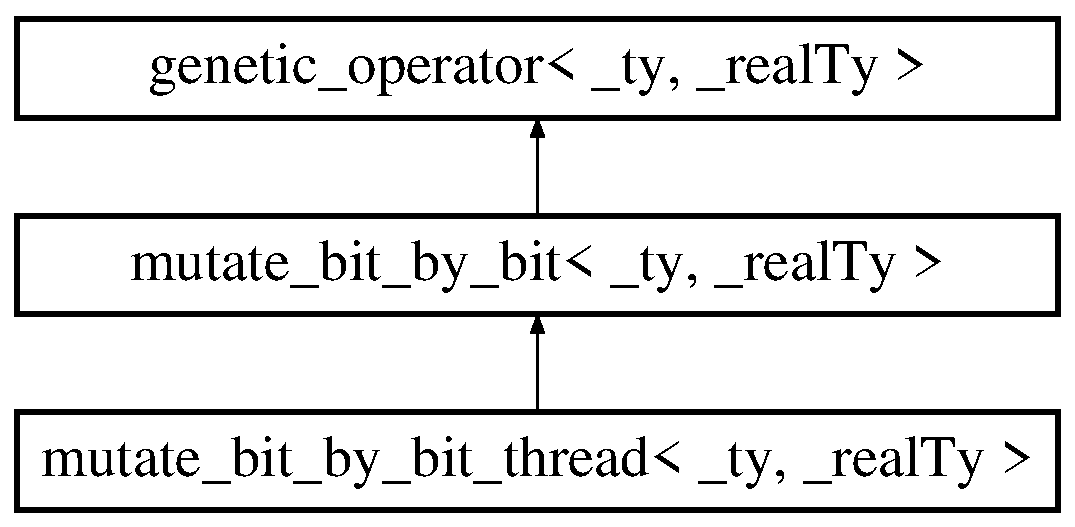
\includegraphics[height=3cm]{classmutate__bit__by__bit}
\end{center}
\end{figure}
\subsection*{Métodos Públicos}
\begin{DoxyCompactItemize}
\item 
\hyperlink{classmutate__bit__by__bit_a14de7465518021a37cfa7e06e19d02f5}{mutate\_\-bit\_\-by\_\-bit} (\hyperlink{classpopulation}{population}$<$ \_\-ty, \_\-realTy $>$ $\ast$pt\_\-to\_\-apply\_\-operator=NULL, const float \&probability=def::genetic\_\-operator::mutate\_\-bit\_\-by\_\-bit::probability)
\item 
virtual const char \& \hyperlink{classmutate__bit__by__bit_a2f8cc52a35943854f24b7534ecd90c7b}{WalkOnPopulationHook} (\hyperlink{classindividual}{individual}$<$ \_\-ty, \_\-realTy $>$ \&id)
\item 
virtual const char \& \hyperlink{classmutate__bit__by__bit_a150b01e7ee79683012f7d60e8c1b9ccc}{WalkOnIndividualHook} (\hyperlink{classcoordinate}{coordinate}$<$ \_\-ty, \_\-realTy $>$ \&coo)
\item 
virtual std::string \hyperlink{classmutate__bit__by__bit_abdab6da2a2b180f14d71f35c895313a4}{GetName} (void)
\end{DoxyCompactItemize}
\subsubsection*{template$<$typename \_\-ty, typename \_\-realTy$>$ class mutate\_\-bit\_\-by\_\-bit$<$ \_\-ty, \_\-realTy $>$}



\subsection{Construtores \& Destrutores}
\hypertarget{classmutate__bit__by__bit_a14de7465518021a37cfa7e06e19d02f5}{
\index{mutate\_\-bit\_\-by\_\-bit@{mutate\_\-bit\_\-by\_\-bit}!mutate\_\-bit\_\-by\_\-bit@{mutate\_\-bit\_\-by\_\-bit}}
\index{mutate\_\-bit\_\-by\_\-bit@{mutate\_\-bit\_\-by\_\-bit}!mutate_bit_by_bit@{mutate\_\-bit\_\-by\_\-bit}}
\subsubsection[{mutate\_\-bit\_\-by\_\-bit}]{\setlength{\rightskip}{0pt plus 5cm}template$<$typename \_\-ty, typename \_\-realTy$>$ {\bf mutate\_\-bit\_\-by\_\-bit}$<$ \_\-ty, \_\-realTy $>$::{\bf mutate\_\-bit\_\-by\_\-bit} ({\bf population}$<$ \_\-ty, \_\-realTy $>$ $\ast$ {\em pt\_\-to\_\-apply\_\-operator} = {\ttfamily NULL}, \/  const float \& {\em probability} = {\ttfamily def::genetic\_\-operator::mutate\_\-bit\_\-by\_\-bit$<$~\_\-ty,~\_\-realTy~$>$::probability})\hspace{0.3cm}{\ttfamily  \mbox{[}inline\mbox{]}}}}
\label{classmutate__bit__by__bit_a14de7465518021a37cfa7e06e19d02f5}
Método contrutor.

pt\_\-to\_\-apply\_\-operator Ponteiro para a população aonde o operador genético será aplicado.  probability Probabilidade do operador genético ser aplicado. 

\subsection{Métodos}
\hypertarget{classmutate__bit__by__bit_abdab6da2a2b180f14d71f35c895313a4}{
\index{mutate\_\-bit\_\-by\_\-bit@{mutate\_\-bit\_\-by\_\-bit}!GetName@{GetName}}
\index{GetName@{GetName}!mutate_bit_by_bit@{mutate\_\-bit\_\-by\_\-bit}}
\subsubsection[{GetName}]{\setlength{\rightskip}{0pt plus 5cm}template$<$typename \_\-ty, typename \_\-realTy$>$ virtual std::string {\bf mutate\_\-bit\_\-by\_\-bit}$<$ \_\-ty, \_\-realTy $>$::GetName (void)\hspace{0.3cm}{\ttfamily  \mbox{[}inline, virtual\mbox{]}}}}
\label{classmutate__bit__by__bit_abdab6da2a2b180f14d71f35c895313a4}
Retorna o nome da classe, usado no padrão AbstractFactory

\begin{DoxyReturn}{Retorna}
Uma string com o nome da classe. 
\end{DoxyReturn}


Reimplementação de \hyperlink{classgenetic__operator_ae0f79368c0b4ad0cff3f608727bd87f5}{genetic\_\-operator$<$ \_\-ty, \_\-realTy $>$}.

\hypertarget{classmutate__bit__by__bit_a150b01e7ee79683012f7d60e8c1b9ccc}{
\index{mutate\_\-bit\_\-by\_\-bit@{mutate\_\-bit\_\-by\_\-bit}!WalkOnIndividualHook@{WalkOnIndividualHook}}
\index{WalkOnIndividualHook@{WalkOnIndividualHook}!mutate_bit_by_bit@{mutate\_\-bit\_\-by\_\-bit}}
\subsubsection[{WalkOnIndividualHook}]{\setlength{\rightskip}{0pt plus 5cm}template$<$typename \_\-ty , typename \_\-realTy $>$ const char \& {\bf mutate\_\-bit\_\-by\_\-bit}$<$ \_\-ty, \_\-realTy $>$::WalkOnIndividualHook ({\bf coordinate}$<$ \_\-ty, \_\-realTy $>$ \& {\em coo})\hspace{0.3cm}{\ttfamily  \mbox{[}inline, virtual\mbox{]}}}}
\label{classmutate__bit__by__bit_a150b01e7ee79683012f7d60e8c1b9ccc}
A operação bit a bit de mutação é realizada nas coordenadas

coo A coordenada em que será aplicado o operador.

\begin{DoxyReturn}{Retorna}
A direção da caminhada sobre os conteiners. 
\end{DoxyReturn}


Implementa \hyperlink{classgenetic__operator_a2124d70b28b35d3114eb3e3ffa72baef}{genetic\_\-operator$<$ \_\-ty, \_\-realTy $>$}.

\hypertarget{classmutate__bit__by__bit_a2f8cc52a35943854f24b7534ecd90c7b}{
\index{mutate\_\-bit\_\-by\_\-bit@{mutate\_\-bit\_\-by\_\-bit}!WalkOnPopulationHook@{WalkOnPopulationHook}}
\index{WalkOnPopulationHook@{WalkOnPopulationHook}!mutate_bit_by_bit@{mutate\_\-bit\_\-by\_\-bit}}
\subsubsection[{WalkOnPopulationHook}]{\setlength{\rightskip}{0pt plus 5cm}template$<$typename \_\-ty, typename \_\-realTy$>$ virtual const char\& {\bf mutate\_\-bit\_\-by\_\-bit}$<$ \_\-ty, \_\-realTy $>$::WalkOnPopulationHook ({\bf individual}$<$ \_\-ty, \_\-realTy $>$ \& {\em id})\hspace{0.3cm}{\ttfamily  \mbox{[}inline, virtual\mbox{]}}}}
\label{classmutate__bit__by__bit_a2f8cc52a35943854f24b7534ecd90c7b}
Nenhuma operação é realizada diretamente nos indivíduos, apenas nas coordenadas

id Indivíduo aonde será aplicado o operador.

\begin{DoxyReturn}{Retorna}
A direção da caminhada sobre os containers. 
\end{DoxyReturn}


Implementa \hyperlink{classgenetic__operator_a3405bb5335111bd675d408aa8db052fa}{genetic\_\-operator$<$ \_\-ty, \_\-realTy $>$}.



A documentação para esta classe foi gerada a partir do seguinte arquivo:\begin{DoxyCompactItemize}
\item 
mutate\_\-bit\_\-by\_\-bit.h\end{DoxyCompactItemize}

\hypertarget{classmutate__bit__by__bit__thread}{
\section{Referência da Template de Classe mutate\_\-bit\_\-by\_\-bit\_\-thread$<$ \_\-ty, \_\-realTy $>$}
\label{classmutate__bit__by__bit__thread}\index{mutate\_\-bit\_\-by\_\-bit\_\-thread@{mutate\_\-bit\_\-by\_\-bit\_\-thread}}
}


{\ttfamily \#include $<$mutate\_\-bit\_\-by\_\-bit\_\-thread.h$>$}

Diagrama de Hierarquia para mutate\_\-bit\_\-by\_\-bit\_\-thread$<$ \_\-ty, \_\-realTy $>$:\begin{figure}[H]
\begin{center}
\leavevmode
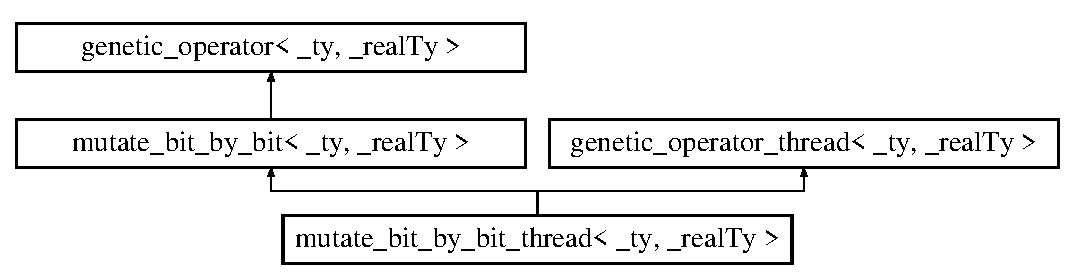
\includegraphics[height=3cm]{classmutate__bit__by__bit__thread}
\end{center}
\end{figure}
\subsection*{Tipos Públicos}
\begin{DoxyCompactItemize}
\item 
typedef boost::mutex::scoped\_\-lock \hyperlink{classmutate__bit__by__bit__thread_a059838b054d4de64b20d33d1db7e89c0}{scoped\_\-lock}
\end{DoxyCompactItemize}
\subsection*{Métodos Públicos}
\begin{DoxyCompactItemize}
\item 
\hyperlink{classmutate__bit__by__bit__thread_a3f2bb991bf06934cb614d2fb91f2bf0a}{mutate\_\-bit\_\-by\_\-bit\_\-thread} (\hyperlink{classpopulation}{population}$<$ \_\-ty, \_\-realTy $>$ $\ast$popPt)
\item 
void \hyperlink{classmutate__bit__by__bit__thread_a13d804deae7d91aa75897068eb733050}{ConsumeAndProduce} (void)
\end{DoxyCompactItemize}
\subsection*{Métodos Protegidos}
\begin{DoxyCompactItemize}
\item 
void \hyperlink{classmutate__bit__by__bit__thread_a452b4832fd083ab19d3f3f65b79bf271}{ApplyMutateOperatorInIndividual} (\hyperlink{classindividual}{individual}$<$ \_\-ty, \_\-realTy $>$ $\ast$id)
\end{DoxyCompactItemize}
\subsection*{Métodos Protegidos Estáticos}
\begin{DoxyCompactItemize}
\item 
static void $\ast$ \hyperlink{classmutate__bit__by__bit__thread_a6f3893ebf8126e17b2f45e694811765f}{CallConsumeAndProduce} (void $\ast$v)
\end{DoxyCompactItemize}


\subsection{Descrição Detalhada}
\subsubsection*{template$<$typename \_\-ty, typename \_\-realTy$>$ class mutate\_\-bit\_\-by\_\-bit\_\-thread$<$ \_\-ty, \_\-realTy $>$}

Classe que define um objeto do tipo operador genético. Este objeto herda os atributos das classes \hyperlink{classgenetic__operator}{genetic\_\-operator} e \hyperlink{classmutate__bit__by__bit}{mutate\_\-bit\_\-by\_\-bit}.


\begin{DoxyTemplParams}{Template Parameters}
\item[{\em \_\-ty}]\item[{\em \_\-realTy}]\end{DoxyTemplParams}


\subsection{Definições de Tipos}
\hypertarget{classmutate__bit__by__bit__thread_a059838b054d4de64b20d33d1db7e89c0}{
\index{mutate\_\-bit\_\-by\_\-bit\_\-thread@{mutate\_\-bit\_\-by\_\-bit\_\-thread}!scoped\_\-lock@{scoped\_\-lock}}
\index{scoped\_\-lock@{scoped\_\-lock}!mutate_bit_by_bit_thread@{mutate\_\-bit\_\-by\_\-bit\_\-thread}}
\subsubsection[{scoped\_\-lock}]{\setlength{\rightskip}{0pt plus 5cm}template$<$typename \_\-ty, typename \_\-realTy$>$ typedef boost::mutex::scoped\_\-lock {\bf mutate\_\-bit\_\-by\_\-bit\_\-thread}$<$ \_\-ty, \_\-realTy $>$::{\bf scoped\_\-lock}}}
\label{classmutate__bit__by__bit__thread_a059838b054d4de64b20d33d1db7e89c0}
Definição do padrão scoped lock. 

Reimplementação de \hyperlink{classgenetic__operator__thread_abe926f8fc2a1548516dad216a1acd4fb}{genetic\_\-operator\_\-thread$<$ \_\-ty, \_\-realTy $>$}.



\subsection{Construtores \& Destrutores}
\hypertarget{classmutate__bit__by__bit__thread_a3f2bb991bf06934cb614d2fb91f2bf0a}{
\index{mutate\_\-bit\_\-by\_\-bit\_\-thread@{mutate\_\-bit\_\-by\_\-bit\_\-thread}!mutate\_\-bit\_\-by\_\-bit\_\-thread@{mutate\_\-bit\_\-by\_\-bit\_\-thread}}
\index{mutate\_\-bit\_\-by\_\-bit\_\-thread@{mutate\_\-bit\_\-by\_\-bit\_\-thread}!mutate_bit_by_bit_thread@{mutate\_\-bit\_\-by\_\-bit\_\-thread}}
\subsubsection[{mutate\_\-bit\_\-by\_\-bit\_\-thread}]{\setlength{\rightskip}{0pt plus 5cm}template$<$typename \_\-ty , typename \_\-realTy $>$ {\bf mutate\_\-bit\_\-by\_\-bit\_\-thread}$<$ \_\-ty, \_\-realTy $>$::{\bf mutate\_\-bit\_\-by\_\-bit\_\-thread} ({\bf population}$<$ \_\-ty, \_\-realTy $>$ $\ast$ {\em popPt})\hspace{0.3cm}{\ttfamily  \mbox{[}inline\mbox{]}}}}
\label{classmutate__bit__by__bit__thread_a3f2bb991bf06934cb614d2fb91f2bf0a}
Método construtor.

popPt Ponteiro para a populção na qual será aplicado o operador. 

\subsection{Métodos}
\hypertarget{classmutate__bit__by__bit__thread_a452b4832fd083ab19d3f3f65b79bf271}{
\index{mutate\_\-bit\_\-by\_\-bit\_\-thread@{mutate\_\-bit\_\-by\_\-bit\_\-thread}!ApplyMutateOperatorInIndividual@{ApplyMutateOperatorInIndividual}}
\index{ApplyMutateOperatorInIndividual@{ApplyMutateOperatorInIndividual}!mutate_bit_by_bit_thread@{mutate\_\-bit\_\-by\_\-bit\_\-thread}}
\subsubsection[{ApplyMutateOperatorInIndividual}]{\setlength{\rightskip}{0pt plus 5cm}template$<$typename \_\-ty , typename \_\-realTy $>$ void {\bf mutate\_\-bit\_\-by\_\-bit\_\-thread}$<$ \_\-ty, \_\-realTy $>$::ApplyMutateOperatorInIndividual ({\bf individual}$<$ \_\-ty, \_\-realTy $>$ $\ast$ {\em id})\hspace{0.3cm}{\ttfamily  \mbox{[}inline, protected\mbox{]}}}}
\label{classmutate__bit__by__bit__thread_a452b4832fd083ab19d3f3f65b79bf271}
Aplica o operador de mutação em um indivíduo

id O indivíduo aonde será aplicado o operador de mutação.

Método que recebe como parâmetro um ponteiro para um indivíduo e aplica o operador de mutação sobre o mesmo. Basicamente o método caminha sobre cada objeto coordenada do indivíduo, e aplica o operador sobre cada coordenada. A probabilidade de mutação de cada bit é definidia no arquivo \hyperlink{definitions_8h}{definitions.h}


\begin{DoxyTemplParams}{Template Parameters}
\item[{\em \_\-ty}]Tipo de cada coordenada para a representação binária \item[{\em \_\-realTy}]Tipo das coordenadas para a representação real  id Ponteiro para o indivíduo no qual será aplicado o operador de mutação bit a bit. \end{DoxyTemplParams}
\hypertarget{classmutate__bit__by__bit__thread_a6f3893ebf8126e17b2f45e694811765f}{
\index{mutate\_\-bit\_\-by\_\-bit\_\-thread@{mutate\_\-bit\_\-by\_\-bit\_\-thread}!CallConsumeAndProduce@{CallConsumeAndProduce}}
\index{CallConsumeAndProduce@{CallConsumeAndProduce}!mutate_bit_by_bit_thread@{mutate\_\-bit\_\-by\_\-bit\_\-thread}}
\subsubsection[{CallConsumeAndProduce}]{\setlength{\rightskip}{0pt plus 5cm}template$<$typename \_\-ty, typename \_\-realTy$>$ static void$\ast$ {\bf mutate\_\-bit\_\-by\_\-bit\_\-thread}$<$ \_\-ty, \_\-realTy $>$::CallConsumeAndProduce (void $\ast$ {\em v})\hspace{0.3cm}{\ttfamily  \mbox{[}inline, static, protected\mbox{]}}}}
\label{classmutate__bit__by__bit__thread_a6f3893ebf8126e17b2f45e694811765f}
Usado para criar as threads

v Ponteiro para o operador que chamará as threads.

\begin{DoxyReturn}{Retorna}
Ponteiro NULL. 
\end{DoxyReturn}
\hypertarget{classmutate__bit__by__bit__thread_a13d804deae7d91aa75897068eb733050}{
\index{mutate\_\-bit\_\-by\_\-bit\_\-thread@{mutate\_\-bit\_\-by\_\-bit\_\-thread}!ConsumeAndProduce@{ConsumeAndProduce}}
\index{ConsumeAndProduce@{ConsumeAndProduce}!mutate_bit_by_bit_thread@{mutate\_\-bit\_\-by\_\-bit\_\-thread}}
\subsubsection[{ConsumeAndProduce}]{\setlength{\rightskip}{0pt plus 5cm}template$<$typename \_\-ty , typename \_\-realTy $>$ void {\bf mutate\_\-bit\_\-by\_\-bit\_\-thread}$<$ \_\-ty, \_\-realTy $>$::ConsumeAndProduce (void)\hspace{0.3cm}{\ttfamily  \mbox{[}inline\mbox{]}}}}
\label{classmutate__bit__by__bit__thread_a13d804deae7d91aa75897068eb733050}
Método a ser executado pelas threads

Método a ser executado pelas threads do operador de mutação bit a bit. O operador remove um indivíduo da sua população, aplica o operador de mutação, e já deposita o mesmo no operador que consome os indivíduos do operador de mutação, que no caso, é o operador de seleção.


\begin{DoxyTemplParams}{Template Parameters}
\item[{\em \_\-ty}]\item[{\em \_\-realTy}]\end{DoxyTemplParams}


A documentação para esta classe foi gerada a partir do seguinte arquivo:\begin{DoxyCompactItemize}
\item 
\hyperlink{mutate__bit__by__bit__thread_8h}{mutate\_\-bit\_\-by\_\-bit\_\-thread.h}\end{DoxyCompactItemize}

\hypertarget{classpopulation}{
\section{Referência da Template de Classe population$<$ \_\-ty, \_\-realTy $>$}
\label{classpopulation}\index{population@{population}}
}


{\ttfamily \#include $<$population.h$>$}

Diagrama de Hierarquia para population$<$ \_\-ty, \_\-realTy $>$:\begin{figure}[H]
\begin{center}
\leavevmode
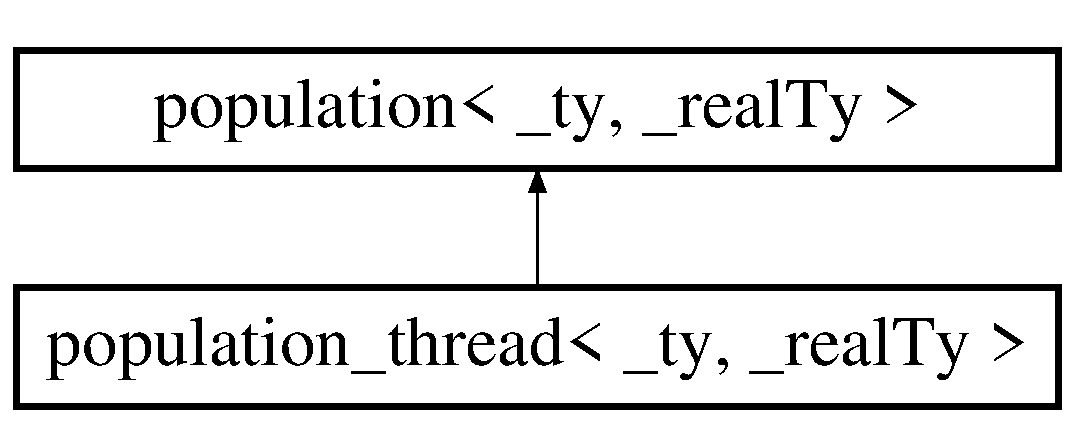
\includegraphics[height=2cm]{classpopulation}
\end{center}
\end{figure}
\subsection*{Tipos Públicos}
\begin{DoxyCompactItemize}
\item 
typedef std::vector$<$ \hyperlink{classindividual}{individual}$<$ \_\-ty, \_\-realTy $>$ $\ast$ $>$ \hyperlink{classpopulation_a487317a079f4b94c650983ccbd0048a5}{\_\-pop}
\item 
typedef std::vector$<$ \hyperlink{classindividual}{individual}$<$ \_\-ty, \_\-realTy $>$ $\ast$ $>$::iterator \hyperlink{classpopulation_aa2f35e7dcc0553a7d2a96e5dca6105e0}{it\_\-}
\item 
typedef std::vector$<$ \hyperlink{classindividual}{individual}$<$ \_\-ty, \_\-realTy $>$ $\ast$ $>$::const\_\-iterator \hyperlink{classpopulation_afcea3753ae2b2e0211f8fdc919c51a71}{const\_\-it\_\-}
\end{DoxyCompactItemize}
\subsection*{Métodos Públicos}
\begin{DoxyCompactItemize}
\item 
\hyperlink{classpopulation_aa497c7bcf82ec82f15cf0ca41f29c153}{population} (const int \&number\_\-ids=def::population::population\_\-size)
\item 
\hyperlink{classpopulation_ab7b5dad1173b0da5b177e6253b66a071}{population} (const \hyperlink{classpopulation}{population}$<$ \_\-ty, \_\-realTy $>$ \&pop)
\item 
\hyperlink{classpopulation_a735c7c86f92155f0deb6034432086d37}{$\sim$population} (void)
\item 
int \hyperlink{classpopulation_a15aee31f3669a3819a025d0c88fd559b}{GetId} (void) const 
\item 
void \hyperlink{classpopulation_aa7803cea8fa30be9c9732d8e81f8aaf4}{SetId} (const int \&new\_\-id)
\item 
int \hyperlink{classpopulation_aa8d33d15eef1966482d052ff509bc638}{GetNumerOfIndividuals} (void) const 
\item 
\_\-realTy \hyperlink{classpopulation_a3c0a549de81a152a15f052e57f106a86}{GetAveragePerformance} (void) const 
\item 
void \hyperlink{classpopulation_a7fb6b0d19740560913aac2eb376c56fb}{SetAveragePerformance} (const \_\-realTy \&new\_\-average)
\item 
\_\-realTy \hyperlink{classpopulation_ac7e0fd101523d1f1db34ae3484a30bf3}{GetSum} (void)
\item 
void \hyperlink{classpopulation_a80e34ba9884327ddc5bafbaedd32014b}{SetSum} (const \_\-realTy \&new\_\-sum)
\item 
\_\-realTy \hyperlink{classpopulation_abe769cd333fa71228e6a89da1171fd93}{GetDeviation} (void) const 
\item 
void \hyperlink{classpopulation_ad0b1614ed94b9eb82a8ca0e24bdc603b}{SetDeviation} (const \_\-realTy \&new\_\-deviation)
\item 
void \hyperlink{classpopulation_a2ddcfb41305717b30051f0aa0a8e240c}{SendGenerationDataToStream} (std::ostream \&os) const 
\item 
\hyperlink{classpopulation_afcea3753ae2b2e0211f8fdc919c51a71}{const\_\-it\_\-} \hyperlink{classpopulation_a4751584859b70770ae44717a43f9ab95}{begin} (void) const 
\item 
\hyperlink{classpopulation_afcea3753ae2b2e0211f8fdc919c51a71}{const\_\-it\_\-} \hyperlink{classpopulation_a38318f9ca5c607490f4d6e92b54d8734}{end} (void) const 
\item 
\hyperlink{classpopulation_aa2f35e7dcc0553a7d2a96e5dca6105e0}{it\_\-} \hyperlink{classpopulation_a7c7bcf224b99227f6ab381dbc9f37c2c}{begin} (void)
\item 
\hyperlink{classpopulation_aa2f35e7dcc0553a7d2a96e5dca6105e0}{it\_\-} \hyperlink{classpopulation_a42a620c96d521b7dcbd091c086258a4c}{end} (void)
\item 
void \hyperlink{classpopulation_ac7b74f6cbb098394df06e1c84de0f260}{SetNewIndividuals} (const \hyperlink{classpopulation_a487317a079f4b94c650983ccbd0048a5}{\_\-pop} \&new\_\-pop)
\item 
\hyperlink{classindividual}{individual}$<$ \_\-ty, \_\-realTy $>$ $\ast$ \hyperlink{classpopulation_a251eb4e8235f4c456e2940fe4a0e4678}{GetWorseId} (void) const 
\item 
\hyperlink{classindividual}{individual}$<$ \_\-ty, \_\-realTy $>$ $\ast$ \hyperlink{classpopulation_a9b2b5de6f220010a0d6c780b7ce04e5b}{GetBestId} (void) const 
\item 
\hyperlink{classpopulation_afcea3753ae2b2e0211f8fdc919c51a71}{const\_\-it\_\-} \hyperlink{classpopulation_a6ca81f5193818b065f792fac9b51f6e3}{operator\mbox{[}$\,$\mbox{]}} (const int \&indice) const 
\item 
bool \hyperlink{classpopulation_a1a847bb47928abf5a0d0a7e4a2ec8c5f}{operator==} (const \hyperlink{classpopulation}{population}$<$ \_\-ty, \_\-realTy $>$ \&pop) const 
\item 
\hyperlink{classindividual}{individual}$<$ \_\-ty, \_\-realTy $>$ $\ast$ \hyperlink{classpopulation_a14c45c3fe1905bcb673919ae251087a9}{operator\mbox{[}$\,$\mbox{]}} (const int \&indice)
\item 
void \hyperlink{classpopulation_aba14d0fb6ceb7499c4fc4838889ba918}{PrintPairs} (void) const 
\item 
void \hyperlink{classpopulation_a20b40816fade14ec740cdc3f22d8066e}{GeneratePopulation} (void)
\item 
void \hyperlink{classpopulation_a10331bd5a9f8f4879cea62ee8b1f28c3}{SetIndividualsValue} (void)
\item 
void \hyperlink{classpopulation_a83be39057000008244d4d7bc947d09fa}{SortPopulation} (void)
\item 
void \hyperlink{classpopulation_a6953ec7e3cd8aa654a1621c515e0d166}{CleanPopulation} (void)
\item 
bool \hyperlink{classpopulation_a23a6d7fca0c7cbaffdcf6cb6cf3239a9}{AddIndividualToPopulation} (\hyperlink{classindividual}{individual}$<$ \_\-ty, \_\-realTy $>$ $\ast$newId)
\item 
bool \hyperlink{classpopulation_a1c227882a579ffe0b2fb049518e1eb85}{RemoveIndividualAt} (const int \&pos)
\item 
void \hyperlink{classpopulation_aa2cbedb9d90d9c660b4a4369857e1c96}{SetNullIndividualAt} (const int \&pos)
\item 
void \hyperlink{classpopulation_a7dd1a669bdbc71381ad2d01ca35c24ae}{UpdateData} (void)
\end{DoxyCompactItemize}
\subsection*{Amigas}
\begin{DoxyCompactItemize}
\item 
\hypertarget{classpopulation_aa6fb88900759771dccfd85d21785fd1b}{
{\footnotesize template$<$typename T , typename U $>$ }\\std::istream \& \hyperlink{classpopulation_aa6fb88900759771dccfd85d21785fd1b}{operator$>$$>$} (std::istream \&is, \hyperlink{classpopulation}{population}$<$ T, U $>$ \&pop)}
\label{classpopulation_aa6fb88900759771dccfd85d21785fd1b}

\begin{DoxyCompactList}\small\item\em Sobrecarga de operadores. \item\end{DoxyCompactList}\item 
\hypertarget{classpopulation_ab134fdc6db277abea408d9dfb410e725}{
{\footnotesize template$<$typename T , typename U $>$ }\\std::ostream \& {\bfseries operator$<$$<$} (std::ostream \&os, const \hyperlink{classpopulation}{population}$<$ T, U $>$ \&pop)}
\label{classpopulation_ab134fdc6db277abea408d9dfb410e725}

\end{DoxyCompactItemize}


\subsection{Descrição Detalhada}
\subsubsection*{template$<$typename \_\-ty, typename \_\-realTy$>$ class population$<$ \_\-ty, \_\-realTy $>$}

Class that encapsulates the concept of a population in a Genetic algorithm optimization method.

Importantan Variables:

\_\-myPop: Container that stores the individuals of the population \_\-bestId,\_\-worseId: Respectivily best and worse individuals of the consteiner \_\-myPop \_\-avarege: Avarage value of the objective function of the population 

\subsection{Definições de Tipos}
\hypertarget{classpopulation_a487317a079f4b94c650983ccbd0048a5}{
\index{population@{population}!\_\-pop@{\_\-pop}}
\index{\_\-pop@{\_\-pop}!population@{population}}
\subsubsection[{\_\-pop}]{\setlength{\rightskip}{0pt plus 5cm}template$<$typename \_\-ty, typename \_\-realTy$>$ typedef std::vector$<${\bf individual}$<$\_\-ty,\_\-realTy$>$$\ast$$>$ {\bf population}$<$ \_\-ty, \_\-realTy $>$::{\bf \_\-pop}}}
\label{classpopulation_a487317a079f4b94c650983ccbd0048a5}
Definição de uma população. \hypertarget{classpopulation_afcea3753ae2b2e0211f8fdc919c51a71}{
\index{population@{population}!const\_\-it\_\-@{const\_\-it\_\-}}
\index{const\_\-it\_\-@{const\_\-it\_\-}!population@{population}}
\subsubsection[{const\_\-it\_\-}]{\setlength{\rightskip}{0pt plus 5cm}template$<$typename \_\-ty, typename \_\-realTy$>$ typedef std::vector$<${\bf individual}$<$\_\-ty,\_\-realTy$>$$\ast$$>$::const\_\-iterator {\bf population}$<$ \_\-ty, \_\-realTy $>$::{\bf const\_\-it\_\-}}}
\label{classpopulation_afcea3753ae2b2e0211f8fdc919c51a71}
Definição de um iterator constante para percorrer o vetor de indivíduos. \hypertarget{classpopulation_aa2f35e7dcc0553a7d2a96e5dca6105e0}{
\index{population@{population}!it\_\-@{it\_\-}}
\index{it\_\-@{it\_\-}!population@{population}}
\subsubsection[{it\_\-}]{\setlength{\rightskip}{0pt plus 5cm}template$<$typename \_\-ty, typename \_\-realTy$>$ typedef std::vector$<${\bf individual}$<$\_\-ty,\_\-realTy$>$$\ast$$>$::iterator {\bf population}$<$ \_\-ty, \_\-realTy $>$::{\bf it\_\-}}}
\label{classpopulation_aa2f35e7dcc0553a7d2a96e5dca6105e0}
Definição de um iterator para percorrer o vetor de indivíduos. 

\subsection{Construtores \& Destrutores}
\hypertarget{classpopulation_aa497c7bcf82ec82f15cf0ca41f29c153}{
\index{population@{population}!population@{population}}
\index{population@{population}!population@{population}}
\subsubsection[{population}]{\setlength{\rightskip}{0pt plus 5cm}template$<$typename \_\-ty , typename \_\-realTy $>$ {\bf population}$<$ \_\-ty, \_\-realTy $>$::{\bf population} (const int \& {\em number\_\-ids} = {\ttfamily def::population$<$~\_\-ty,~\_\-realTy~$>$::population\_\-size})\hspace{0.3cm}{\ttfamily  \mbox{[}inline\mbox{]}}}}
\label{classpopulation_aa497c7bcf82ec82f15cf0ca41f29c153}
Método contrutor que recebe apenas o tamanho da população, ou seja, o número de indivíduos da mesma.

number\_\-ids O número de indivíduos da população. \hypertarget{classpopulation_ab7b5dad1173b0da5b177e6253b66a071}{
\index{population@{population}!population@{population}}
\index{population@{population}!population@{population}}
\subsubsection[{population}]{\setlength{\rightskip}{0pt plus 5cm}template$<$typename \_\-ty , typename \_\-realTy $>$ {\bf population}$<$ \_\-ty, \_\-realTy $>$::{\bf population} (const {\bf population}$<$ \_\-ty, \_\-realTy $>$ \& {\em pop})\hspace{0.3cm}{\ttfamily  \mbox{[}inline\mbox{]}}}}
\label{classpopulation_ab7b5dad1173b0da5b177e6253b66a071}
Construtor de cópia.

pop População a ser copiada. \hypertarget{classpopulation_a735c7c86f92155f0deb6034432086d37}{
\index{population@{population}!$\sim$population@{$\sim$population}}
\index{$\sim$population@{$\sim$population}!population@{population}}
\subsubsection[{$\sim$population}]{\setlength{\rightskip}{0pt plus 5cm}template$<$typename \_\-ty , typename \_\-realTy $>$ {\bf population}$<$ \_\-ty, \_\-realTy $>$::$\sim${\bf population} (void)\hspace{0.3cm}{\ttfamily  \mbox{[}inline\mbox{]}}}}
\label{classpopulation_a735c7c86f92155f0deb6034432086d37}
Método destrutor. 

\subsection{Métodos}
\hypertarget{classpopulation_a23a6d7fca0c7cbaffdcf6cb6cf3239a9}{
\index{population@{population}!AddIndividualToPopulation@{AddIndividualToPopulation}}
\index{AddIndividualToPopulation@{AddIndividualToPopulation}!population@{population}}
\subsubsection[{AddIndividualToPopulation}]{\setlength{\rightskip}{0pt plus 5cm}template$<$typename \_\-ty , typename \_\-realTy $>$ bool {\bf population}$<$ \_\-ty, \_\-realTy $>$::AddIndividualToPopulation ({\bf individual}$<$ \_\-ty, \_\-realTy $>$ $\ast$ {\em newId})\hspace{0.3cm}{\ttfamily  \mbox{[}inline\mbox{]}}}}
\label{classpopulation_a23a6d7fca0c7cbaffdcf6cb6cf3239a9}
Adiciona um indivíduo no vetor caso o vetor não esteja cheio, e retorna se foi possível adicionar o novo indivíduo

newId Novo indivíduo a ser adicionado.

\begin{DoxyReturn}{Retorna}
True se a inserção foi realzada com sucesso, false caso contrário. 
\end{DoxyReturn}
\hypertarget{classpopulation_a7c7bcf224b99227f6ab381dbc9f37c2c}{
\index{population@{population}!begin@{begin}}
\index{begin@{begin}!population@{population}}
\subsubsection[{begin}]{\setlength{\rightskip}{0pt plus 5cm}template$<$typename \_\-ty, typename \_\-realTy$>$ {\bf it\_\-} {\bf population}$<$ \_\-ty, \_\-realTy $>$::begin (void)\hspace{0.3cm}{\ttfamily  \mbox{[}inline\mbox{]}}}}
\label{classpopulation_a7c7bcf224b99227f6ab381dbc9f37c2c}
Retorna um iterator para manipular os indivíduos da população.

\begin{DoxyReturn}{Retorna}
Um iterator para o começo do container que armazena os indivíduos. 
\end{DoxyReturn}
\hypertarget{classpopulation_a4751584859b70770ae44717a43f9ab95}{
\index{population@{population}!begin@{begin}}
\index{begin@{begin}!population@{population}}
\subsubsection[{begin}]{\setlength{\rightskip}{0pt plus 5cm}template$<$typename \_\-ty, typename \_\-realTy$>$ {\bf const\_\-it\_\-} {\bf population}$<$ \_\-ty, \_\-realTy $>$::begin (void) const\hspace{0.3cm}{\ttfamily  \mbox{[}inline\mbox{]}}}}
\label{classpopulation_a4751584859b70770ae44717a43f9ab95}
Retorna um iterator para manipular os indivíduos da população.

\begin{DoxyReturn}{Retorna}
Um iterator para o começo do container que armazena os indivíduos. 
\end{DoxyReturn}
\hypertarget{classpopulation_a6953ec7e3cd8aa654a1621c515e0d166}{
\index{population@{population}!CleanPopulation@{CleanPopulation}}
\index{CleanPopulation@{CleanPopulation}!population@{population}}
\subsubsection[{CleanPopulation}]{\setlength{\rightskip}{0pt plus 5cm}template$<$typename \_\-ty , typename \_\-realTy $>$ void {\bf population}$<$ \_\-ty, \_\-realTy $>$::CleanPopulation (void)\hspace{0.3cm}{\ttfamily  \mbox{[}inline\mbox{]}}}}
\label{classpopulation_a6953ec7e3cd8aa654a1621c515e0d166}
Limpa o container de indivíduos da população. \hypertarget{classpopulation_a42a620c96d521b7dcbd091c086258a4c}{
\index{population@{population}!end@{end}}
\index{end@{end}!population@{population}}
\subsubsection[{end}]{\setlength{\rightskip}{0pt plus 5cm}template$<$typename \_\-ty, typename \_\-realTy$>$ {\bf it\_\-} {\bf population}$<$ \_\-ty, \_\-realTy $>$::end (void)\hspace{0.3cm}{\ttfamily  \mbox{[}inline\mbox{]}}}}
\label{classpopulation_a42a620c96d521b7dcbd091c086258a4c}
Retorna um iterator para manipular os indivíduos da população.

\begin{DoxyReturn}{Retorna}
Um iterator para o fim do container que armazena os indivíduos. 
\end{DoxyReturn}
\hypertarget{classpopulation_a38318f9ca5c607490f4d6e92b54d8734}{
\index{population@{population}!end@{end}}
\index{end@{end}!population@{population}}
\subsubsection[{end}]{\setlength{\rightskip}{0pt plus 5cm}template$<$typename \_\-ty, typename \_\-realTy$>$ {\bf const\_\-it\_\-} {\bf population}$<$ \_\-ty, \_\-realTy $>$::end (void) const\hspace{0.3cm}{\ttfamily  \mbox{[}inline\mbox{]}}}}
\label{classpopulation_a38318f9ca5c607490f4d6e92b54d8734}
Retorna um iterator para manipular os indivíduos da população.

\begin{DoxyReturn}{Retorna}
Um iterator para o fim do container que armazena os indivíduos. 
\end{DoxyReturn}
\hypertarget{classpopulation_a20b40816fade14ec740cdc3f22d8066e}{
\index{population@{population}!GeneratePopulation@{GeneratePopulation}}
\index{GeneratePopulation@{GeneratePopulation}!population@{population}}
\subsubsection[{GeneratePopulation}]{\setlength{\rightskip}{0pt plus 5cm}template$<$typename \_\-ty , typename \_\-realTy $>$ void {\bf population}$<$ \_\-ty, \_\-realTy $>$::GeneratePopulation (void)\hspace{0.3cm}{\ttfamily  \mbox{[}inline\mbox{]}}}}
\label{classpopulation_a20b40816fade14ec740cdc3f22d8066e}
Gera uma população de indivíduos aleatórios. \hypertarget{classpopulation_a3c0a549de81a152a15f052e57f106a86}{
\index{population@{population}!GetAveragePerformance@{GetAveragePerformance}}
\index{GetAveragePerformance@{GetAveragePerformance}!population@{population}}
\subsubsection[{GetAveragePerformance}]{\setlength{\rightskip}{0pt plus 5cm}template$<$typename \_\-ty, typename \_\-realTy$>$ \_\-realTy {\bf population}$<$ \_\-ty, \_\-realTy $>$::GetAveragePerformance (void) const\hspace{0.3cm}{\ttfamily  \mbox{[}inline\mbox{]}}}}
\label{classpopulation_a3c0a549de81a152a15f052e57f106a86}
Método de interface (get).

\begin{DoxyReturn}{Retorna}
O valor médio do fitness dos indivíduos da população. 
\end{DoxyReturn}
\hypertarget{classpopulation_a9b2b5de6f220010a0d6c780b7ce04e5b}{
\index{population@{population}!GetBestId@{GetBestId}}
\index{GetBestId@{GetBestId}!population@{population}}
\subsubsection[{GetBestId}]{\setlength{\rightskip}{0pt plus 5cm}template$<$typename \_\-ty, typename \_\-realTy$>$ {\bf individual}$<$\_\-ty,\_\-realTy$>$$\ast$ {\bf population}$<$ \_\-ty, \_\-realTy $>$::GetBestId (void) const\hspace{0.3cm}{\ttfamily  \mbox{[}inline\mbox{]}}}}
\label{classpopulation_a9b2b5de6f220010a0d6c780b7ce04e5b}
Método de interface (get).

\begin{DoxyReturn}{Retorna}
Um ponteiro para o indivíduo com o melhor fitness da população. 
\end{DoxyReturn}
\hypertarget{classpopulation_abe769cd333fa71228e6a89da1171fd93}{
\index{population@{population}!GetDeviation@{GetDeviation}}
\index{GetDeviation@{GetDeviation}!population@{population}}
\subsubsection[{GetDeviation}]{\setlength{\rightskip}{0pt plus 5cm}template$<$typename \_\-ty, typename \_\-realTy$>$ \_\-realTy {\bf population}$<$ \_\-ty, \_\-realTy $>$::GetDeviation (void) const\hspace{0.3cm}{\ttfamily  \mbox{[}inline\mbox{]}}}}
\label{classpopulation_abe769cd333fa71228e6a89da1171fd93}
Método de interface (get).

\begin{DoxyReturn}{Retorna}
O valor da variância do fitness dos indivíduos da população. 
\end{DoxyReturn}
\hypertarget{classpopulation_a15aee31f3669a3819a025d0c88fd559b}{
\index{population@{population}!GetId@{GetId}}
\index{GetId@{GetId}!population@{population}}
\subsubsection[{GetId}]{\setlength{\rightskip}{0pt plus 5cm}template$<$typename \_\-ty, typename \_\-realTy$>$ int {\bf population}$<$ \_\-ty, \_\-realTy $>$::GetId (void) const\hspace{0.3cm}{\ttfamily  \mbox{[}inline\mbox{]}}}}
\label{classpopulation_a15aee31f3669a3819a025d0c88fd559b}
Método de interface (get).

\begin{DoxyReturn}{Retorna}
O inteiro que identifica unicamente um indivíduo. 
\end{DoxyReturn}
\hypertarget{classpopulation_aa8d33d15eef1966482d052ff509bc638}{
\index{population@{population}!GetNumerOfIndividuals@{GetNumerOfIndividuals}}
\index{GetNumerOfIndividuals@{GetNumerOfIndividuals}!population@{population}}
\subsubsection[{GetNumerOfIndividuals}]{\setlength{\rightskip}{0pt plus 5cm}template$<$typename \_\-ty, typename \_\-realTy$>$ int {\bf population}$<$ \_\-ty, \_\-realTy $>$::GetNumerOfIndividuals (void) const\hspace{0.3cm}{\ttfamily  \mbox{[}inline\mbox{]}}}}
\label{classpopulation_aa8d33d15eef1966482d052ff509bc638}
Método de interface (get).

\begin{DoxyReturn}{Retorna}
O número de indivíduos da população. 
\end{DoxyReturn}
\hypertarget{classpopulation_ac7e0fd101523d1f1db34ae3484a30bf3}{
\index{population@{population}!GetSum@{GetSum}}
\index{GetSum@{GetSum}!population@{population}}
\subsubsection[{GetSum}]{\setlength{\rightskip}{0pt plus 5cm}template$<$typename \_\-ty, typename \_\-realTy$>$ \_\-realTy {\bf population}$<$ \_\-ty, \_\-realTy $>$::GetSum (void)\hspace{0.3cm}{\ttfamily  \mbox{[}inline\mbox{]}}}}
\label{classpopulation_ac7e0fd101523d1f1db34ae3484a30bf3}
Método de interface (get).

\begin{DoxyReturn}{Retorna}
A soma dos valores de fitness de todos os indivíduos da população. 
\end{DoxyReturn}
\hypertarget{classpopulation_a251eb4e8235f4c456e2940fe4a0e4678}{
\index{population@{population}!GetWorseId@{GetWorseId}}
\index{GetWorseId@{GetWorseId}!population@{population}}
\subsubsection[{GetWorseId}]{\setlength{\rightskip}{0pt plus 5cm}template$<$typename \_\-ty, typename \_\-realTy$>$ {\bf individual}$<$\_\-ty,\_\-realTy$>$$\ast$ {\bf population}$<$ \_\-ty, \_\-realTy $>$::GetWorseId (void) const\hspace{0.3cm}{\ttfamily  \mbox{[}inline\mbox{]}}}}
\label{classpopulation_a251eb4e8235f4c456e2940fe4a0e4678}
Método de interface (get).

\begin{DoxyReturn}{Retorna}
Um ponteiro para o indivíduo com o pior fitness da população. 
\end{DoxyReturn}
\hypertarget{classpopulation_a1a847bb47928abf5a0d0a7e4a2ec8c5f}{
\index{population@{population}!operator==@{operator==}}
\index{operator==@{operator==}!population@{population}}
\subsubsection[{operator==}]{\setlength{\rightskip}{0pt plus 5cm}template$<$typename \_\-ty , typename \_\-realTy $>$ bool {\bf population}$<$ \_\-ty, \_\-realTy $>$::operator== (const {\bf population}$<$ \_\-ty, \_\-realTy $>$ \& {\em pop}) const\hspace{0.3cm}{\ttfamily  \mbox{[}inline\mbox{]}}}}
\label{classpopulation_a1a847bb47928abf5a0d0a7e4a2ec8c5f}
Operador de igualdade. Retorna se dois indivíduos têm o mesmo fitness.

pop A população que se deseja comparar o fitness.

\begin{DoxyReturn}{Retorna}
True caso os fitnesses sejam iguais, false caso contrário. 
\end{DoxyReturn}
\hypertarget{classpopulation_a14c45c3fe1905bcb673919ae251087a9}{
\index{population@{population}!operator\mbox{[}\mbox{]}@{operator[]}}
\index{operator\mbox{[}\mbox{]}@{operator[]}!population@{population}}
\subsubsection[{operator[]}]{\setlength{\rightskip}{0pt plus 5cm}template$<$typename \_\-ty, typename \_\-realTy$>$ {\bf individual}$<$\_\-ty,\_\-realTy$>$$\ast$ {\bf population}$<$ \_\-ty, \_\-realTy $>$::operator\mbox{[}$\,$\mbox{]} (const int \& {\em indice})\hspace{0.3cm}{\ttfamily  \mbox{[}inline\mbox{]}}}}
\label{classpopulation_a14c45c3fe1905bcb673919ae251087a9}
Operador de acesso aleatório. Acesso um indivíduo em determinado índice do container de indivíduos.

indice O índice do container do indivíduo que se deseja acessar.

\begin{DoxyReturn}{Retorna}
Um ponteiro para o indivíduo que se deseja acessar. 
\end{DoxyReturn}
\hypertarget{classpopulation_a6ca81f5193818b065f792fac9b51f6e3}{
\index{population@{population}!operator\mbox{[}\mbox{]}@{operator[]}}
\index{operator\mbox{[}\mbox{]}@{operator[]}!population@{population}}
\subsubsection[{operator[]}]{\setlength{\rightskip}{0pt plus 5cm}template$<$typename \_\-ty, typename \_\-realTy$>$ {\bf const\_\-it\_\-} {\bf population}$<$ \_\-ty, \_\-realTy $>$::operator\mbox{[}$\,$\mbox{]} (const int \& {\em indice}) const\hspace{0.3cm}{\ttfamily  \mbox{[}inline\mbox{]}}}}
\label{classpopulation_a6ca81f5193818b065f792fac9b51f6e3}
Operador de acesso aleatório. Acesso um indivíduo em determinado índice do container de indivíduos.

indice O índice do container do indivíduo que se deseja acessar.

\begin{DoxyReturn}{Retorna}
Um iterator para o indivíduo que se deseja acessar. 
\end{DoxyReturn}
\hypertarget{classpopulation_aba14d0fb6ceb7499c4fc4838889ba918}{
\index{population@{population}!PrintPairs@{PrintPairs}}
\index{PrintPairs@{PrintPairs}!population@{population}}
\subsubsection[{PrintPairs}]{\setlength{\rightskip}{0pt plus 5cm}template$<$typename \_\-ty , typename \_\-realTy $>$ void {\bf population}$<$ \_\-ty, \_\-realTy $>$::PrintPairs (void) const\hspace{0.3cm}{\ttfamily  \mbox{[}inline\mbox{]}}}}
\label{classpopulation_aba14d0fb6ceb7499c4fc4838889ba918}
Imprime os pares da população na saída padrão. \hypertarget{classpopulation_a1c227882a579ffe0b2fb049518e1eb85}{
\index{population@{population}!RemoveIndividualAt@{RemoveIndividualAt}}
\index{RemoveIndividualAt@{RemoveIndividualAt}!population@{population}}
\subsubsection[{RemoveIndividualAt}]{\setlength{\rightskip}{0pt plus 5cm}template$<$typename \_\-ty , typename \_\-realTy $>$ bool {\bf population}$<$ \_\-ty, \_\-realTy $>$::RemoveIndividualAt (const int \& {\em pos})\hspace{0.3cm}{\ttfamily  \mbox{[}inline\mbox{]}}}}
\label{classpopulation_a1c227882a579ffe0b2fb049518e1eb85}
Remove o indivíduo da posição pos da população

pos A posição no container de indivíduos do indivíduo a ser removido.

\begin{DoxyReturn}{Retorna}
True se a remoção foi realizada com sucesso, false caso contrário. 
\end{DoxyReturn}
\hypertarget{classpopulation_a2ddcfb41305717b30051f0aa0a8e240c}{
\index{population@{population}!SendGenerationDataToStream@{SendGenerationDataToStream}}
\index{SendGenerationDataToStream@{SendGenerationDataToStream}!population@{population}}
\subsubsection[{SendGenerationDataToStream}]{\setlength{\rightskip}{0pt plus 5cm}template$<$typename \_\-ty, typename \_\-realTy$>$ void {\bf population}$<$ \_\-ty, \_\-realTy $>$::SendGenerationDataToStream (std::ostream \& {\em os}) const\hspace{0.3cm}{\ttfamily  \mbox{[}inline\mbox{]}}}}
\label{classpopulation_a2ddcfb41305717b30051f0aa0a8e240c}
Envia os dados da população (fitness, variancia, etc) para a stream.

os A stream para onde são enviado os dados. \hypertarget{classpopulation_a7fb6b0d19740560913aac2eb376c56fb}{
\index{population@{population}!SetAveragePerformance@{SetAveragePerformance}}
\index{SetAveragePerformance@{SetAveragePerformance}!population@{population}}
\subsubsection[{SetAveragePerformance}]{\setlength{\rightskip}{0pt plus 5cm}template$<$typename \_\-ty, typename \_\-realTy$>$ void {\bf population}$<$ \_\-ty, \_\-realTy $>$::SetAveragePerformance (const \_\-realTy \& {\em new\_\-average})\hspace{0.3cm}{\ttfamily  \mbox{[}inline\mbox{]}}}}
\label{classpopulation_a7fb6b0d19740560913aac2eb376c56fb}
Método de interface (set).

new\_\-average O novo valor médio do fitness dos indivíduos da população. \hypertarget{classpopulation_ad0b1614ed94b9eb82a8ca0e24bdc603b}{
\index{population@{population}!SetDeviation@{SetDeviation}}
\index{SetDeviation@{SetDeviation}!population@{population}}
\subsubsection[{SetDeviation}]{\setlength{\rightskip}{0pt plus 5cm}template$<$typename \_\-ty, typename \_\-realTy$>$ void {\bf population}$<$ \_\-ty, \_\-realTy $>$::SetDeviation (const \_\-realTy \& {\em new\_\-deviation})\hspace{0.3cm}{\ttfamily  \mbox{[}inline\mbox{]}}}}
\label{classpopulation_ad0b1614ed94b9eb82a8ca0e24bdc603b}
Método de interface (set).

new\_\-deviation O novo valor da variância do fitness dos indivíduos da população. \hypertarget{classpopulation_aa7803cea8fa30be9c9732d8e81f8aaf4}{
\index{population@{population}!SetId@{SetId}}
\index{SetId@{SetId}!population@{population}}
\subsubsection[{SetId}]{\setlength{\rightskip}{0pt plus 5cm}template$<$typename \_\-ty, typename \_\-realTy$>$ void {\bf population}$<$ \_\-ty, \_\-realTy $>$::SetId (const int \& {\em new\_\-id})\hspace{0.3cm}{\ttfamily  \mbox{[}inline\mbox{]}}}}
\label{classpopulation_aa7803cea8fa30be9c9732d8e81f8aaf4}
Método de interface (set).

new\_\-id O novo valor que identifica o indivíduo unicamente. \hypertarget{classpopulation_a10331bd5a9f8f4879cea62ee8b1f28c3}{
\index{population@{population}!SetIndividualsValue@{SetIndividualsValue}}
\index{SetIndividualsValue@{SetIndividualsValue}!population@{population}}
\subsubsection[{SetIndividualsValue}]{\setlength{\rightskip}{0pt plus 5cm}template$<$typename \_\-ty , typename \_\-realTy $>$ void {\bf population}$<$ \_\-ty, \_\-realTy $>$::SetIndividualsValue (void)\hspace{0.3cm}{\ttfamily  \mbox{[}inline\mbox{]}}}}
\label{classpopulation_a10331bd5a9f8f4879cea62ee8b1f28c3}
Seta o valor da função objetivo para cada indivíduo da população \hypertarget{classpopulation_ac7b74f6cbb098394df06e1c84de0f260}{
\index{population@{population}!SetNewIndividuals@{SetNewIndividuals}}
\index{SetNewIndividuals@{SetNewIndividuals}!population@{population}}
\subsubsection[{SetNewIndividuals}]{\setlength{\rightskip}{0pt plus 5cm}template$<$typename \_\-ty, typename \_\-realTy$>$ void {\bf population}$<$ \_\-ty, \_\-realTy $>$::SetNewIndividuals (const {\bf \_\-pop} \& {\em new\_\-pop})}}
\label{classpopulation_ac7b74f6cbb098394df06e1c84de0f260}
Seta os novos indivíduos da população.

new\_\-pop População que contém os indivíduos que formarão a nova população. \hypertarget{classpopulation_aa2cbedb9d90d9c660b4a4369857e1c96}{
\index{population@{population}!SetNullIndividualAt@{SetNullIndividualAt}}
\index{SetNullIndividualAt@{SetNullIndividualAt}!population@{population}}
\subsubsection[{SetNullIndividualAt}]{\setlength{\rightskip}{0pt plus 5cm}template$<$typename \_\-ty , typename \_\-realTy $>$ void {\bf population}$<$ \_\-ty, \_\-realTy $>$::SetNullIndividualAt (const int \& {\em pos})\hspace{0.3cm}{\ttfamily  \mbox{[}inline\mbox{]}}}}
\label{classpopulation_aa2cbedb9d90d9c660b4a4369857e1c96}
Seta um individuo como nulo (usado antes de remover para manter o individuo antigo)

pos A posição no container de indivíduos do indivíduo a ser removido. \hypertarget{classpopulation_a80e34ba9884327ddc5bafbaedd32014b}{
\index{population@{population}!SetSum@{SetSum}}
\index{SetSum@{SetSum}!population@{population}}
\subsubsection[{SetSum}]{\setlength{\rightskip}{0pt plus 5cm}template$<$typename \_\-ty, typename \_\-realTy$>$ void {\bf population}$<$ \_\-ty, \_\-realTy $>$::SetSum (const \_\-realTy \& {\em new\_\-sum})\hspace{0.3cm}{\ttfamily  \mbox{[}inline\mbox{]}}}}
\label{classpopulation_a80e34ba9884327ddc5bafbaedd32014b}
Método de interface (set).

new\_\-sum O novovalor da soma a ser setado. \hypertarget{classpopulation_a83be39057000008244d4d7bc947d09fa}{
\index{population@{population}!SortPopulation@{SortPopulation}}
\index{SortPopulation@{SortPopulation}!population@{population}}
\subsubsection[{SortPopulation}]{\setlength{\rightskip}{0pt plus 5cm}template$<$typename \_\-ty, typename \_\-realTy$>$ void {\bf population}$<$ \_\-ty, \_\-realTy $>$::SortPopulation (void)\hspace{0.3cm}{\ttfamily  \mbox{[}inline\mbox{]}}}}
\label{classpopulation_a83be39057000008244d4d7bc947d09fa}
Ordena o vetor de indivíduos da população. \hypertarget{classpopulation_a7dd1a669bdbc71381ad2d01ca35c24ae}{
\index{population@{population}!UpdateData@{UpdateData}}
\index{UpdateData@{UpdateData}!population@{population}}
\subsubsection[{UpdateData}]{\setlength{\rightskip}{0pt plus 5cm}template$<$typename \_\-ty , typename \_\-realTy $>$ void {\bf population}$<$ \_\-ty, \_\-realTy $>$::UpdateData (void)\hspace{0.3cm}{\ttfamily  \mbox{[}inline\mbox{]}}}}
\label{classpopulation_a7dd1a669bdbc71381ad2d01ca35c24ae}
Atualiza os dados da nova geração da população 

A documentação para esta classe foi gerada a partir do seguinte arquivo:\begin{DoxyCompactItemize}
\item 
\hyperlink{population_8h}{population.h}\end{DoxyCompactItemize}

\hypertarget{structpopulation__compare}{
\section{Referência da Template de Estrutura population\_\-compare$<$ \_\-ty, \_\-realTy $>$}
\label{structpopulation__compare}\index{population\_\-compare@{population\_\-compare}}
}


{\ttfamily \#include $<$population.h$>$}

\subsection*{Métodos Públicos}
\begin{DoxyCompactItemize}
\item 
\hypertarget{structpopulation__compare_aad5bd281f88104395004ee4e62bd0c10}{
bool {\bfseries operator()} (const \hyperlink{classindividual}{individual}$<$ \_\-ty, \_\-realTy $>$ $\ast$a, const \hyperlink{classindividual}{individual}$<$ \_\-ty, \_\-realTy $>$ $\ast$b) const }
\label{structpopulation__compare_aad5bd281f88104395004ee4e62bd0c10}

\end{DoxyCompactItemize}


\subsection{Descrição Detalhada}
\subsubsection*{template$<$typename \_\-ty, typename \_\-realTy$>$ struct population\_\-compare$<$ \_\-ty, \_\-realTy $>$}

Function object used in the sort method to sort the elements of container that stores the individuals of the population. 

A documentação para esta estrutura foi gerada a partir do seguinte arquivo:\begin{DoxyCompactItemize}
\item 
\hyperlink{population_8h}{population.h}\end{DoxyCompactItemize}

\hypertarget{classpopulation__thread}{
\section{Referência da Template de Classe population\_\-thread$<$ \_\-ty, \_\-realTy $>$}
\label{classpopulation__thread}\index{population\_\-thread@{population\_\-thread}}
}
Diagrama de Hierarquia para population\_\-thread$<$ \_\-ty, \_\-realTy $>$:\begin{figure}[H]
\begin{center}
\leavevmode
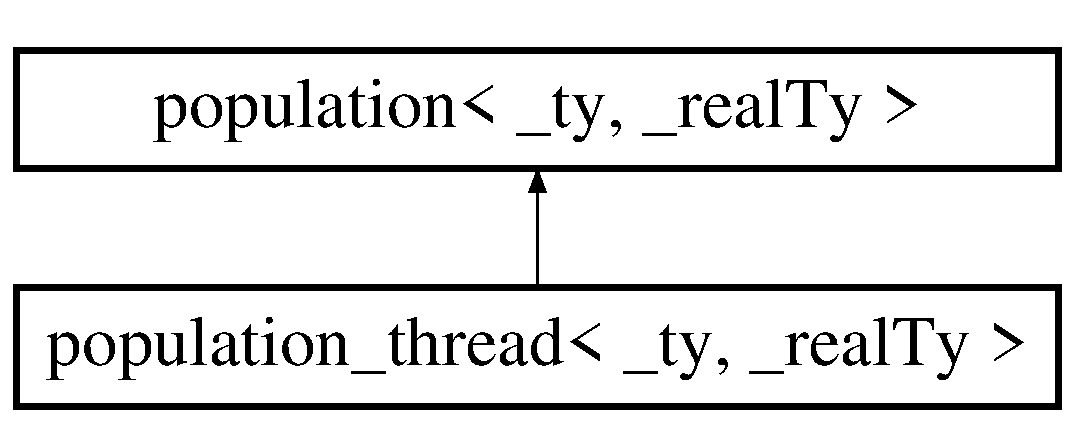
\includegraphics[height=2cm]{classpopulation__thread}
\end{center}
\end{figure}
\subsection*{Métodos Públicos}
\begin{DoxyCompactItemize}
\item 
\hypertarget{classpopulation__thread_a9ff695442d2529a10aec61636ae5dc40}{
void {\bfseries SetIndividualsValue} (typename \hyperlink{classpopulation}{population}$<$ \_\-ty, \_\-realTy $>$::\hyperlink{classpopulation_aa2f35e7dcc0553a7d2a96e5dca6105e0}{it\_\-} first, typename \hyperlink{classpopulation}{population}$<$ \_\-ty, \_\-realTy $>$::\hyperlink{classpopulation_aa2f35e7dcc0553a7d2a96e5dca6105e0}{it\_\-} second)}
\label{classpopulation__thread_a9ff695442d2529a10aec61636ae5dc40}

\end{DoxyCompactItemize}
\subsubsection*{template$<$typename \_\-ty, typename \_\-realTy$>$ class population\_\-thread$<$ \_\-ty, \_\-realTy $>$}



A documentação para esta classe foi gerada a partir do seguinte arquivo:\begin{DoxyCompactItemize}
\item 
population\_\-thread.h\end{DoxyCompactItemize}

\hypertarget{classselection__by__roulette}{
\section{Referência da Template de Classe selection\_\-by\_\-roulette$<$ \_\-ty, \_\-realTy $>$}
\label{classselection__by__roulette}\index{selection\_\-by\_\-roulette@{selection\_\-by\_\-roulette}}
}


{\ttfamily \#include $<$selection\_\-by\_\-roulette.h$>$}

Diagrama de Hierarquia para selection\_\-by\_\-roulette$<$ \_\-ty, \_\-realTy $>$:\begin{figure}[H]
\begin{center}
\leavevmode
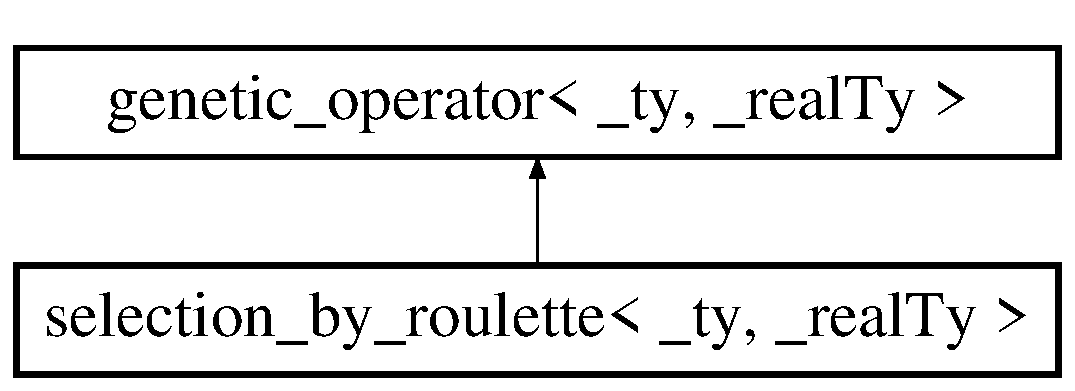
\includegraphics[height=2cm]{classselection__by__roulette}
\end{center}
\end{figure}
\subsection*{Tipos Públicos}
\begin{DoxyCompactItemize}
\item 
typedef std::vector$<$ std::pair$<$ \_\-realTy, \hyperlink{classindividual}{individual}$<$ \_\-ty, \_\-realTy $>$ $\ast$ $>$ $>$ \hyperlink{classselection__by__roulette_a4c224a095113f38dce7d98f10d8c0833}{\_\-RouletteTy}
\item 
typedef std::vector$<$ std::pair$<$ \_\-realTy, \hyperlink{classindividual}{individual}$<$ \_\-ty, \_\-realTy $>$ $\ast$ $>$ $>$::iterator \hyperlink{classselection__by__roulette_a557d2432eb36aba61aa31a9e4b0dcb54}{it\_\-}
\item 
typedef std::vector$<$ std::pair$<$ \_\-realTy, \hyperlink{classindividual}{individual}$<$ \_\-ty, \_\-realTy $>$ $\ast$ $>$ $>$::const\_\-iterator \hyperlink{classselection__by__roulette_ac64df0d86cf8396ce91df17d9ce27f0e}{const\_\-it\_\-}
\end{DoxyCompactItemize}
\subsection*{Métodos Públicos}
\begin{DoxyCompactItemize}
\item 
\hyperlink{classselection__by__roulette_a043cefe0479622491fea593c7f28ddfa}{selection\_\-by\_\-roulette} (\hyperlink{classpopulation}{population}$<$ \_\-ty, \_\-realTy $>$ $\ast$pt\_\-to\_\-apply\_\-operator=NULL)
\item 
virtual std::string \hyperlink{classselection__by__roulette_a137f1a757ab4d71a0ca0bdba7f9f35d0}{GetName} (void)
\item 
virtual const char \& \hyperlink{classselection__by__roulette_abb536fd7b63a452a2ebd8e7572bfc4d8}{WalkOnIndividualHook} (\hyperlink{classcoordinate}{coordinate}$<$ \_\-ty, \_\-realTy $>$ \&coo)
\item 
virtual const char \& \hyperlink{classselection__by__roulette_a98be3d54afb87450f190615f7da330e9}{WalkOnPopulationHook} (\hyperlink{classindividual}{individual}$<$ \_\-ty, \_\-realTy $>$ \&id)
\item 
\hyperlink{classselection__by__roulette_ac64df0d86cf8396ce91df17d9ce27f0e}{const\_\-it\_\-} \hyperlink{classselection__by__roulette_a8d04a76229aa2d0c68c1a945e77d8e19}{begin} (void) const 
\item 
\hyperlink{classselection__by__roulette_ac64df0d86cf8396ce91df17d9ce27f0e}{const\_\-it\_\-} \hyperlink{classselection__by__roulette_a2abe33c34280ba81f0f0dab12c8e875b}{end} (void) const 
\end{DoxyCompactItemize}
\subsection*{Métodos Protegidos}
\begin{DoxyCompactItemize}
\item 
virtual void \hyperlink{classselection__by__roulette_ac3db5bbe67ee2aa4e1942fd983d3cc80}{GenerateRoulette} (void)
\item 
virtual void \hyperlink{classselection__by__roulette_ae19e7e752f54ab03983be567c8d10392}{RotateRoulette} (void)
\end{DoxyCompactItemize}


\subsection{Descrição Detalhada}
\subsubsection*{template$<$typename \_\-ty, typename \_\-realTy$>$ class selection\_\-by\_\-roulette$<$ \_\-ty, \_\-realTy $>$}

Classe template que encapsula os métodos e atributos de um operador genético de seleção por torneio. Herda da classe \hyperlink{classgenetic__operator}{genetic\_\-operator}. Os métods principais são \hyperlink{classselection__by__roulette_ac3db5bbe67ee2aa4e1942fd983d3cc80}{GenerateRoulette()} e \hyperlink{classselection__by__roulette_ae19e7e752f54ab03983be567c8d10392}{RotateRoulette()}.


\begin{DoxyTemplParams}{Template Parameters}
\item[{\em \_\-ty}]\item[{\em \_\-realTy}]\end{DoxyTemplParams}


\subsection{Definições de Tipos}
\hypertarget{classselection__by__roulette_a4c224a095113f38dce7d98f10d8c0833}{
\index{selection\_\-by\_\-roulette@{selection\_\-by\_\-roulette}!\_\-RouletteTy@{\_\-RouletteTy}}
\index{\_\-RouletteTy@{\_\-RouletteTy}!selection_by_roulette@{selection\_\-by\_\-roulette}}
\subsubsection[{\_\-RouletteTy}]{\setlength{\rightskip}{0pt plus 5cm}template$<$typename \_\-ty , typename \_\-realTy $>$ typedef std::vector$<$std::pair$<$\_\-realTy,{\bf individual}$<$\_\-ty,\_\-realTy$>$$\ast$$>$ $>$ {\bf selection\_\-by\_\-roulette}$<$ \_\-ty, \_\-realTy $>$::{\bf \_\-RouletteTy}}}
\label{classselection__by__roulette_a4c224a095113f38dce7d98f10d8c0833}
Definição do container que armazena uma roleta. \hypertarget{classselection__by__roulette_ac64df0d86cf8396ce91df17d9ce27f0e}{
\index{selection\_\-by\_\-roulette@{selection\_\-by\_\-roulette}!const\_\-it\_\-@{const\_\-it\_\-}}
\index{const\_\-it\_\-@{const\_\-it\_\-}!selection_by_roulette@{selection\_\-by\_\-roulette}}
\subsubsection[{const\_\-it\_\-}]{\setlength{\rightskip}{0pt plus 5cm}template$<$typename \_\-ty , typename \_\-realTy $>$ typedef std::vector$<$std::pair$<$\_\-realTy,{\bf individual}$<$\_\-ty,\_\-realTy$>$$\ast$$>$ $>$::const\_\-iterator {\bf selection\_\-by\_\-roulette}$<$ \_\-ty, \_\-realTy $>$::{\bf const\_\-it\_\-}}}
\label{classselection__by__roulette_ac64df0d86cf8396ce91df17d9ce27f0e}
Definição para um iterator constante que percorre o container da roleta. \hypertarget{classselection__by__roulette_a557d2432eb36aba61aa31a9e4b0dcb54}{
\index{selection\_\-by\_\-roulette@{selection\_\-by\_\-roulette}!it\_\-@{it\_\-}}
\index{it\_\-@{it\_\-}!selection_by_roulette@{selection\_\-by\_\-roulette}}
\subsubsection[{it\_\-}]{\setlength{\rightskip}{0pt plus 5cm}template$<$typename \_\-ty , typename \_\-realTy $>$ typedef std::vector$<$std::pair$<$\_\-realTy,{\bf individual}$<$\_\-ty,\_\-realTy$>$$\ast$$>$ $>$::iterator {\bf selection\_\-by\_\-roulette}$<$ \_\-ty, \_\-realTy $>$::{\bf it\_\-}}}
\label{classselection__by__roulette_a557d2432eb36aba61aa31a9e4b0dcb54}
Definição para um iterator que percorre o container da roleta. 

\subsection{Construtores \& Destrutores}
\hypertarget{classselection__by__roulette_a043cefe0479622491fea593c7f28ddfa}{
\index{selection\_\-by\_\-roulette@{selection\_\-by\_\-roulette}!selection\_\-by\_\-roulette@{selection\_\-by\_\-roulette}}
\index{selection\_\-by\_\-roulette@{selection\_\-by\_\-roulette}!selection_by_roulette@{selection\_\-by\_\-roulette}}
\subsubsection[{selection\_\-by\_\-roulette}]{\setlength{\rightskip}{0pt plus 5cm}template$<$typename \_\-ty , typename \_\-realTy $>$ {\bf selection\_\-by\_\-roulette}$<$ \_\-ty, \_\-realTy $>$::{\bf selection\_\-by\_\-roulette} ({\bf population}$<$ \_\-ty, \_\-realTy $>$ $\ast$ {\em pt\_\-to\_\-apply\_\-operator} = {\ttfamily NULL})\hspace{0.3cm}{\ttfamily  \mbox{[}inline\mbox{]}}}}
\label{classselection__by__roulette_a043cefe0479622491fea593c7f28ddfa}
Método construtor.

pt\_\-to\_\-apply\_\-operator Ponteiro para a população na qual será aplicado o operador. 

\subsection{Métodos}
\hypertarget{classselection__by__roulette_a8d04a76229aa2d0c68c1a945e77d8e19}{
\index{selection\_\-by\_\-roulette@{selection\_\-by\_\-roulette}!begin@{begin}}
\index{begin@{begin}!selection_by_roulette@{selection\_\-by\_\-roulette}}
\subsubsection[{begin}]{\setlength{\rightskip}{0pt plus 5cm}template$<$typename \_\-ty , typename \_\-realTy $>$ {\bf const\_\-it\_\-} {\bf selection\_\-by\_\-roulette}$<$ \_\-ty, \_\-realTy $>$::begin (void) const\hspace{0.3cm}{\ttfamily  \mbox{[}inline\mbox{]}}}}
\label{classselection__by__roulette_a8d04a76229aa2d0c68c1a945e77d8e19}
Método que retorna um iterator para percorrer a roleta.

\begin{DoxyReturn}{Retorna}
Iterator para o começo do container que armazena a roleta. 
\end{DoxyReturn}
\hypertarget{classselection__by__roulette_a2abe33c34280ba81f0f0dab12c8e875b}{
\index{selection\_\-by\_\-roulette@{selection\_\-by\_\-roulette}!end@{end}}
\index{end@{end}!selection_by_roulette@{selection\_\-by\_\-roulette}}
\subsubsection[{end}]{\setlength{\rightskip}{0pt plus 5cm}template$<$typename \_\-ty , typename \_\-realTy $>$ {\bf const\_\-it\_\-} {\bf selection\_\-by\_\-roulette}$<$ \_\-ty, \_\-realTy $>$::end (void) const\hspace{0.3cm}{\ttfamily  \mbox{[}inline\mbox{]}}}}
\label{classselection__by__roulette_a2abe33c34280ba81f0f0dab12c8e875b}
Métod que retorna um iterator para percorre a roleta.

\begin{DoxyReturn}{Retorna}
Iterator para o fim da roleta. 
\end{DoxyReturn}
\hypertarget{classselection__by__roulette_ac3db5bbe67ee2aa4e1942fd983d3cc80}{
\index{selection\_\-by\_\-roulette@{selection\_\-by\_\-roulette}!GenerateRoulette@{GenerateRoulette}}
\index{GenerateRoulette@{GenerateRoulette}!selection_by_roulette@{selection\_\-by\_\-roulette}}
\subsubsection[{GenerateRoulette}]{\setlength{\rightskip}{0pt plus 5cm}template$<$typename \_\-ty , typename \_\-realTy $>$ void {\bf selection\_\-by\_\-roulette}$<$ \_\-ty, \_\-realTy $>$::GenerateRoulette (void)\hspace{0.3cm}{\ttfamily  \mbox{[}inline, protected, virtual\mbox{]}}}}
\label{classselection__by__roulette_ac3db5bbe67ee2aa4e1942fd983d3cc80}
Constrói a roleta(preenche \_\-myRoulette) \hypertarget{classselection__by__roulette_a137f1a757ab4d71a0ca0bdba7f9f35d0}{
\index{selection\_\-by\_\-roulette@{selection\_\-by\_\-roulette}!GetName@{GetName}}
\index{GetName@{GetName}!selection_by_roulette@{selection\_\-by\_\-roulette}}
\subsubsection[{GetName}]{\setlength{\rightskip}{0pt plus 5cm}template$<$typename \_\-ty , typename \_\-realTy $>$ virtual std::string {\bf selection\_\-by\_\-roulette}$<$ \_\-ty, \_\-realTy $>$::GetName (void)\hspace{0.3cm}{\ttfamily  \mbox{[}inline, virtual\mbox{]}}}}
\label{classselection__by__roulette_a137f1a757ab4d71a0ca0bdba7f9f35d0}
Retorna o nome da classe para o padrão AbstractFactory

\begin{DoxyReturn}{Retorna}
Uma string com o nome da classe. 
\end{DoxyReturn}


Reimplementação de \hyperlink{classgenetic__operator_ae0f79368c0b4ad0cff3f608727bd87f5}{genetic\_\-operator$<$ \_\-ty, \_\-realTy $>$}.

\hypertarget{classselection__by__roulette_ae19e7e752f54ab03983be567c8d10392}{
\index{selection\_\-by\_\-roulette@{selection\_\-by\_\-roulette}!RotateRoulette@{RotateRoulette}}
\index{RotateRoulette@{RotateRoulette}!selection_by_roulette@{selection\_\-by\_\-roulette}}
\subsubsection[{RotateRoulette}]{\setlength{\rightskip}{0pt plus 5cm}template$<$typename \_\-ty , typename \_\-realTy $>$ void {\bf selection\_\-by\_\-roulette}$<$ \_\-ty, \_\-realTy $>$::RotateRoulette (void)\hspace{0.3cm}{\ttfamily  \mbox{[}inline, protected, virtual\mbox{]}}}}
\label{classselection__by__roulette_ae19e7e752f54ab03983be567c8d10392}
Realiza a seleção propriamente dita, ou seja roda a roleta \hypertarget{classselection__by__roulette_abb536fd7b63a452a2ebd8e7572bfc4d8}{
\index{selection\_\-by\_\-roulette@{selection\_\-by\_\-roulette}!WalkOnIndividualHook@{WalkOnIndividualHook}}
\index{WalkOnIndividualHook@{WalkOnIndividualHook}!selection_by_roulette@{selection\_\-by\_\-roulette}}
\subsubsection[{WalkOnIndividualHook}]{\setlength{\rightskip}{0pt plus 5cm}template$<$typename \_\-ty , typename \_\-realTy $>$ virtual const char\& {\bf selection\_\-by\_\-roulette}$<$ \_\-ty, \_\-realTy $>$::WalkOnIndividualHook ({\bf coordinate}$<$ \_\-ty, \_\-realTy $>$ \& {\em coo})\hspace{0.3cm}{\ttfamily  \mbox{[}inline, virtual\mbox{]}}}}
\label{classselection__by__roulette_abb536fd7b63a452a2ebd8e7572bfc4d8}
O método de seleção por roleta não realiza nenhuma operação direta sobre as coordenadas

coo A coordenada onde seria aplicado o operador.

\begin{DoxyReturn}{Retorna}
A direção de caminhada do vetor. 
\end{DoxyReturn}


Implementa \hyperlink{classgenetic__operator_a2124d70b28b35d3114eb3e3ffa72baef}{genetic\_\-operator$<$ \_\-ty, \_\-realTy $>$}.

\hypertarget{classselection__by__roulette_a98be3d54afb87450f190615f7da330e9}{
\index{selection\_\-by\_\-roulette@{selection\_\-by\_\-roulette}!WalkOnPopulationHook@{WalkOnPopulationHook}}
\index{WalkOnPopulationHook@{WalkOnPopulationHook}!selection_by_roulette@{selection\_\-by\_\-roulette}}
\subsubsection[{WalkOnPopulationHook}]{\setlength{\rightskip}{0pt plus 5cm}template$<$typename \_\-ty , typename \_\-realTy $>$ const char \& {\bf selection\_\-by\_\-roulette}$<$ \_\-ty, \_\-realTy $>$::WalkOnPopulationHook ({\bf individual}$<$ \_\-ty, \_\-realTy $>$ \& {\em id})\hspace{0.3cm}{\ttfamily  \mbox{[}inline, virtual\mbox{]}}}}
\label{classselection__by__roulette_a98be3d54afb87450f190615f7da330e9}
O método de seleção por roleta realiza operações diretamente nos indivíduos

id O indivíduo aonde será aplicado o operador de seleção.

\begin{DoxyReturn}{Retorna}
A direção da caminhada do vetor. 
\end{DoxyReturn}


Implementa \hyperlink{classgenetic__operator_a3405bb5335111bd675d408aa8db052fa}{genetic\_\-operator$<$ \_\-ty, \_\-realTy $>$}.



A documentação para esta classe foi gerada a partir do seguinte arquivo:\begin{DoxyCompactItemize}
\item 
\hyperlink{selection__by__roulette_8h}{selection\_\-by\_\-roulette.h}\end{DoxyCompactItemize}

\hypertarget{classselection__by__tournament}{
\section{Referência da Template de Classe selection\_\-by\_\-tournament$<$ \_\-ty, \_\-realTy $>$}
\label{classselection__by__tournament}\index{selection\_\-by\_\-tournament@{selection\_\-by\_\-tournament}}
}


{\ttfamily \#include $<$selection\_\-by\_\-tournament.h$>$}

Diagrama de Hierarquia para selection\_\-by\_\-tournament$<$ \_\-ty, \_\-realTy $>$:\begin{figure}[H]
\begin{center}
\leavevmode
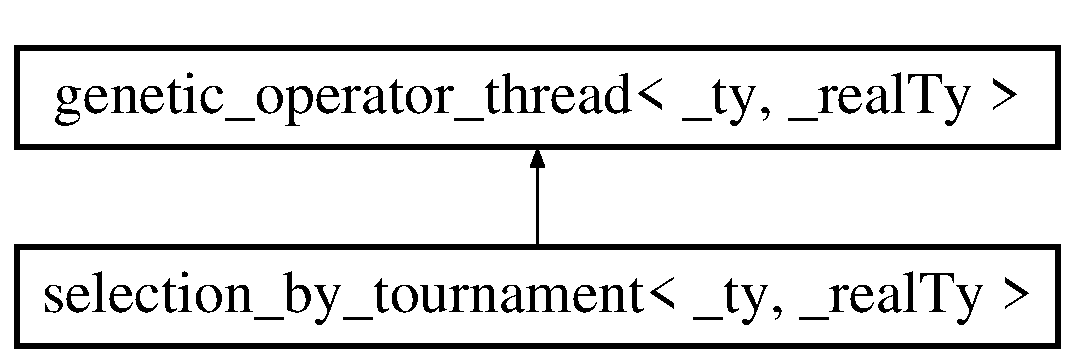
\includegraphics[height=2cm]{classselection__by__tournament}
\end{center}
\end{figure}
\subsection*{Tipos Públicos}
\begin{DoxyCompactItemize}
\item 
typedef boost::mutex::scoped\_\-lock \hyperlink{classselection__by__tournament_a0ba2a47db6a59696b51f19341719c3fd}{scoped\_\-lock}
\end{DoxyCompactItemize}
\subsection*{Métodos Públicos}
\begin{DoxyCompactItemize}
\item 
\hyperlink{classselection__by__tournament_a511f69a870e3bb1fdcf7aa8d48383c15}{selection\_\-by\_\-tournament} (\hyperlink{classpopulation}{population}$<$ \_\-ty, \_\-realTy $>$ $\ast$popPt)
\item 
\hyperlink{classselection__by__tournament_a4865e086f5a9f3aeb6991814f13f7eda}{$\sim$selection\_\-by\_\-tournament} ()
\item 
void \hyperlink{classselection__by__tournament_aa2a32fdcbd6365eea3e40a565c9cff3a}{Select} (void)
\item 
void \hyperlink{classselection__by__tournament_a3e16cf77dd481a3ce1a01ac4edffa4ba}{ReadyToReceive} (void)
\end{DoxyCompactItemize}
\subsection*{Métodos Públicos Estáticos}
\begin{DoxyCompactItemize}
\item 
static void $\ast$ \hyperlink{classselection__by__tournament_ad754f7c3afa1443bfed139265cd506c1}{CallSelect} (\hyperlink{classselection__by__tournament}{selection\_\-by\_\-tournament}$<$ \_\-ty, \_\-realTy $>$ $\ast$v)
\end{DoxyCompactItemize}


\subsection{Descrição Detalhada}
\subsubsection*{template$<$typename \_\-ty, typename \_\-realTy$>$ class selection\_\-by\_\-tournament$<$ \_\-ty, \_\-realTy $>$}

Classe que implementa a interface de um operador genético de seleção por torneio. As threads do operador executam o método \hyperlink{classselection__by__tournament_aa2a32fdcbd6365eea3e40a565c9cff3a}{Select()}. Como o operador de seleção é um gargalo na implementação atual ele espera


\begin{DoxyTemplParams}{Template Parameters}
\item[{\em \_\-ty}]\item[{\em \_\-realTy}]\end{DoxyTemplParams}


\subsection{Definições de Tipos}
\hypertarget{classselection__by__tournament_a0ba2a47db6a59696b51f19341719c3fd}{
\index{selection\_\-by\_\-tournament@{selection\_\-by\_\-tournament}!scoped\_\-lock@{scoped\_\-lock}}
\index{scoped\_\-lock@{scoped\_\-lock}!selection_by_tournament@{selection\_\-by\_\-tournament}}
\subsubsection[{scoped\_\-lock}]{\setlength{\rightskip}{0pt plus 5cm}template$<$typename \_\-ty, typename \_\-realTy$>$ typedef boost::mutex::scoped\_\-lock {\bf selection\_\-by\_\-tournament}$<$ \_\-ty, \_\-realTy $>$::{\bf scoped\_\-lock}}}
\label{classselection__by__tournament_a0ba2a47db6a59696b51f19341719c3fd}
Definição do padrão scoped lock. 

Reimplementação de \hyperlink{classgenetic__operator__thread_abe926f8fc2a1548516dad216a1acd4fb}{genetic\_\-operator\_\-thread$<$ \_\-ty, \_\-realTy $>$}.



\subsection{Construtores \& Destrutores}
\hypertarget{classselection__by__tournament_a511f69a870e3bb1fdcf7aa8d48383c15}{
\index{selection\_\-by\_\-tournament@{selection\_\-by\_\-tournament}!selection\_\-by\_\-tournament@{selection\_\-by\_\-tournament}}
\index{selection\_\-by\_\-tournament@{selection\_\-by\_\-tournament}!selection_by_tournament@{selection\_\-by\_\-tournament}}
\subsubsection[{selection\_\-by\_\-tournament}]{\setlength{\rightskip}{0pt plus 5cm}template$<$typename \_\-ty , typename \_\-realTy $>$ {\bf selection\_\-by\_\-tournament}$<$ \_\-ty, \_\-realTy $>$::{\bf selection\_\-by\_\-tournament} ({\bf population}$<$ \_\-ty, \_\-realTy $>$ $\ast$ {\em popPt})\hspace{0.3cm}{\ttfamily  \mbox{[}inline\mbox{]}}}}
\label{classselection__by__tournament_a511f69a870e3bb1fdcf7aa8d48383c15}
Método construtor.

popPt Ponteiro para a população onde será aplicado o operador. \hypertarget{classselection__by__tournament_a4865e086f5a9f3aeb6991814f13f7eda}{
\index{selection\_\-by\_\-tournament@{selection\_\-by\_\-tournament}!$\sim$selection\_\-by\_\-tournament@{$\sim$selection\_\-by\_\-tournament}}
\index{$\sim$selection\_\-by\_\-tournament@{$\sim$selection\_\-by\_\-tournament}!selection_by_tournament@{selection\_\-by\_\-tournament}}
\subsubsection[{$\sim$selection\_\-by\_\-tournament}]{\setlength{\rightskip}{0pt plus 5cm}template$<$typename \_\-ty, typename \_\-realTy$>$ {\bf selection\_\-by\_\-tournament}$<$ \_\-ty, \_\-realTy $>$::$\sim${\bf selection\_\-by\_\-tournament} ()}}
\label{classselection__by__tournament_a4865e086f5a9f3aeb6991814f13f7eda}
Método destrutor. 

\subsection{Métodos}
\hypertarget{classselection__by__tournament_ad754f7c3afa1443bfed139265cd506c1}{
\index{selection\_\-by\_\-tournament@{selection\_\-by\_\-tournament}!CallSelect@{CallSelect}}
\index{CallSelect@{CallSelect}!selection_by_tournament@{selection\_\-by\_\-tournament}}
\subsubsection[{CallSelect}]{\setlength{\rightskip}{0pt plus 5cm}template$<$typename \_\-ty , typename \_\-realTy $>$ void $\ast$ {\bf selection\_\-by\_\-tournament}$<$ \_\-ty, \_\-realTy $>$::CallSelect ({\bf selection\_\-by\_\-tournament}$<$ \_\-ty, \_\-realTy $>$ $\ast$ {\em v})\hspace{0.3cm}{\ttfamily  \mbox{[}inline, static\mbox{]}}}}
\label{classselection__by__tournament_ad754f7c3afa1443bfed139265cd506c1}
Método que chama as threads.

v Ponteiro para o operador.

\begin{DoxyReturn}{Retorna}
Ponteiro NULL. 
\end{DoxyReturn}
\hypertarget{classselection__by__tournament_a3e16cf77dd481a3ce1a01ac4edffa4ba}{
\index{selection\_\-by\_\-tournament@{selection\_\-by\_\-tournament}!ReadyToReceive@{ReadyToReceive}}
\index{ReadyToReceive@{ReadyToReceive}!selection_by_tournament@{selection\_\-by\_\-tournament}}
\subsubsection[{ReadyToReceive}]{\setlength{\rightskip}{0pt plus 5cm}template$<$typename \_\-ty , typename \_\-realTy $>$ void {\bf selection\_\-by\_\-tournament}$<$ \_\-ty, \_\-realTy $>$::ReadyToReceive (void)\hspace{0.3cm}{\ttfamily  \mbox{[}inline, virtual\mbox{]}}}}
\label{classselection__by__tournament_a3e16cf77dd481a3ce1a01ac4edffa4ba}
Função que implementa a variável de condição para receber indivíduos 

Reimplementação de \hyperlink{classgenetic__operator__thread_a7c86cee81334320d496fb196920fcc10}{genetic\_\-operator\_\-thread$<$ \_\-ty, \_\-realTy $>$}.

\hypertarget{classselection__by__tournament_aa2a32fdcbd6365eea3e40a565c9cff3a}{
\index{selection\_\-by\_\-tournament@{selection\_\-by\_\-tournament}!Select@{Select}}
\index{Select@{Select}!selection_by_tournament@{selection\_\-by\_\-tournament}}
\subsubsection[{Select}]{\setlength{\rightskip}{0pt plus 5cm}template$<$typename \_\-ty , typename \_\-realTy $>$ void {\bf selection\_\-by\_\-tournament}$<$ \_\-ty, \_\-realTy $>$::Select (void)\hspace{0.3cm}{\ttfamily  \mbox{[}inline\mbox{]}}}}
\label{classselection__by__tournament_aa2a32fdcbd6365eea3e40a565c9cff3a}
Realiza o torneio efetivamente após a avaliação da funções objetivo 

A documentação para esta classe foi gerada a partir do seguinte arquivo:\begin{DoxyCompactItemize}
\item 
\hyperlink{selection__by__tournament_8h}{selection\_\-by\_\-tournament.h}\end{DoxyCompactItemize}

\hypertarget{classsemaphore}{
\section{Referência da Classe semaphore}
\label{classsemaphore}\index{semaphore@{semaphore}}
}


{\ttfamily \#include $<$semaphore.h$>$}

\subsection*{Tipos Públicos}
\begin{DoxyCompactItemize}
\item 
typedef boost::mutex::scoped\_\-lock \hyperlink{classsemaphore_ad4d360a8eabfead011d7ce5394c4dd2a}{scoped\_\-lock}
\end{DoxyCompactItemize}
\subsection*{Métodos Públicos}
\begin{DoxyCompactItemize}
\item 
\hyperlink{classsemaphore_a77d85322407545b8ccc4a85b920d90c1}{semaphore} (const unsigned int \&initCount, const unsigned int \&maxCount)
\item 
void \hyperlink{classsemaphore_af0e430d192c44be1d65f5a4fd8cb91a4}{wait} (void)
\item 
void \hyperlink{classsemaphore_a14c3b9f4312c43d9400905c938752665}{post} (void)
\end{DoxyCompactItemize}


\subsection{Descrição Detalhada}
Classe que encapsula os conceitos de um semáforo. Foi necessário a realização desta classe pois não existe um semáforo na boost, com apenas os métodos \hyperlink{classsemaphore_a14c3b9f4312c43d9400905c938752665}{post()} e \hyperlink{classsemaphore_af0e430d192c44be1d65f5a4fd8cb91a4}{wait()} como na pthreads. 

\subsection{Definições de Tipos}
\hypertarget{classsemaphore_ad4d360a8eabfead011d7ce5394c4dd2a}{
\index{semaphore@{semaphore}!scoped\_\-lock@{scoped\_\-lock}}
\index{scoped\_\-lock@{scoped\_\-lock}!semaphore@{semaphore}}
\subsubsection[{scoped\_\-lock}]{\setlength{\rightskip}{0pt plus 5cm}typedef boost::mutex::scoped\_\-lock {\bf semaphore::scoped\_\-lock}}}
\label{classsemaphore_ad4d360a8eabfead011d7ce5394c4dd2a}
Definição do padrão de projeto scoped lock. 

\subsection{Construtores \& Destrutores}
\hypertarget{classsemaphore_a77d85322407545b8ccc4a85b920d90c1}{
\index{semaphore@{semaphore}!semaphore@{semaphore}}
\index{semaphore@{semaphore}!semaphore@{semaphore}}
\subsubsection[{semaphore}]{\setlength{\rightskip}{0pt plus 5cm}semaphore::semaphore (const unsigned int \& {\em initCount}, \/  const unsigned int \& {\em maxCount})\hspace{0.3cm}{\ttfamily  \mbox{[}inline\mbox{]}}}}
\label{classsemaphore_a77d85322407545b8ccc4a85b920d90c1}
Método construtor.

initCount Valor inicial do semáforo.  maxCount Valor máximo do semáforo. 

\subsection{Métodos}
\hypertarget{classsemaphore_a14c3b9f4312c43d9400905c938752665}{
\index{semaphore@{semaphore}!post@{post}}
\index{post@{post}!semaphore@{semaphore}}
\subsubsection[{post}]{\setlength{\rightskip}{0pt plus 5cm}void semaphore::post (void)\hspace{0.3cm}{\ttfamily  \mbox{[}inline\mbox{]}}}}
\label{classsemaphore_a14c3b9f4312c43d9400905c938752665}
Método que decrementa o semáfor, até o valor zero. \hypertarget{classsemaphore_af0e430d192c44be1d65f5a4fd8cb91a4}{
\index{semaphore@{semaphore}!wait@{wait}}
\index{wait@{wait}!semaphore@{semaphore}}
\subsubsection[{wait}]{\setlength{\rightskip}{0pt plus 5cm}void semaphore::wait (void)\hspace{0.3cm}{\ttfamily  \mbox{[}inline\mbox{]}}}}
\label{classsemaphore_af0e430d192c44be1d65f5a4fd8cb91a4}
Método que incremnta o semáforo até o valor máximo. 

A documentação para esta classe foi gerada a partir do seguinte arquivo:\begin{DoxyCompactItemize}
\item 
\hyperlink{semaphore_8h}{semaphore.h}\end{DoxyCompactItemize}

\chapter{Arquivos}
\hypertarget{coordinate_8h}{
\section{Referência do Arquivo coordinate.h}
\label{coordinate_8h}\index{coordinate.h@{coordinate.h}}
}


Arquivo que contêm as definições da classe template coordinate.  


{\ttfamily \#include $<$string$>$}\par
{\ttfamily \#include $<$cmath$>$}\par
{\ttfamily \#include \char`\"{}definitions.h\char`\"{}}\par
{\ttfamily \#include $<$iostream$>$}\par
{\ttfamily \#include $<$stdio.h$>$}\par
{\ttfamily \#include $<$stdlib.h$>$}\par
{\ttfamily \#include $<$time.h$>$}\par
\subsection*{Componentes}
\begin{DoxyCompactItemize}
\item 
class \hyperlink{classcoordinate}{coordinate$<$ \_\-ty, \_\-realTy $>$}
\end{DoxyCompactItemize}
\subsection*{Funções}
\begin{DoxyCompactItemize}
\item 
{\footnotesize template$<$typename T , typename U $>$ }\\std::istream \& \hyperlink{coordinate_8h_aacb2e8f6ef327786248a961828b53fa5}{operator$>$$>$} (std::istream \&is, \hyperlink{classcoordinate}{coordinate}$<$ T, U $>$ \&coo)
\item 
{\footnotesize template$<$typename T , typename U $>$ }\\std::ostream \& \hyperlink{coordinate_8h_ac6da0a94290e6364c27e4dff1a52f5e5}{operator$<$$<$} (std::ostream \&os, const \hyperlink{classcoordinate}{coordinate}$<$ T, U $>$ \&coo)
\end{DoxyCompactItemize}


\subsection{Descrição Detalhada}
Arquivo que contêm as definições da classe template coordinate. \begin{DoxyAuthor}{Autor}
Pedro Pazzini 
\end{DoxyAuthor}
\begin{DoxyVersion}{Versão}
0.0.1 
\end{DoxyVersion}
\begin{DoxyDate}{Data}
2010-\/01-\/21 
\end{DoxyDate}


\subsection{Funções}
\hypertarget{coordinate_8h_ac6da0a94290e6364c27e4dff1a52f5e5}{
\index{coordinate.h@{coordinate.h}!operator$<$$<$@{operator$<$$<$}}
\index{operator$<$$<$@{operator$<$$<$}!coordinate.h@{coordinate.h}}
\subsubsection[{operator$<$$<$}]{\setlength{\rightskip}{0pt plus 5cm}template$<$typename T , typename U $>$ std::ostream\& operator$<$$<$ (std::ostream \& {\em os}, \/  const {\bf coordinate}$<$ T, U $>$ \& {\em coo})\hspace{0.3cm}{\ttfamily  \mbox{[}inline\mbox{]}}}}
\label{coordinate_8h_ac6da0a94290e6364c27e4dff1a52f5e5}
Operador de fluxo de entrada. Recebe os atributos do objeto coordenada da stream, e os seta no objeto do tipo coordenada passado como parâmetro


\begin{DoxyTemplParams}{Template Parameters}
\item[{\em T}]\item[{\em U}]os O objeto stream que carrega os atributos.  coo O objeto coordenada que recebe os atributos da stream\end{DoxyTemplParams}
\begin{DoxyReturn}{Retorna}
O mesmo objeto stream passado como parâmetro, para possibilitar o encadeamento do operador 
\end{DoxyReturn}
\hypertarget{coordinate_8h_aacb2e8f6ef327786248a961828b53fa5}{
\index{coordinate.h@{coordinate.h}!operator$>$$>$@{operator$>$$>$}}
\index{operator$>$$>$@{operator$>$$>$}!coordinate.h@{coordinate.h}}
\subsubsection[{operator$>$$>$}]{\setlength{\rightskip}{0pt plus 5cm}template$<$typename T , typename U $>$ std::istream\& operator$>$$>$ (std::istream \& {\em is}, \/  {\bf coordinate}$<$ T, U $>$ \& {\em coo})\hspace{0.3cm}{\ttfamily  \mbox{[}inline\mbox{]}}}}
\label{coordinate_8h_aacb2e8f6ef327786248a961828b53fa5}
Operador de fluxo de saída. Imprime na stream os atributos do objeto coordenada.


\begin{DoxyTemplParams}{Template Parameters}
\item[{\em T}]\item[{\em U}]is A stream que recebe os atributos  coo A coordenada que possui os atributos que serão passados para a stream\end{DoxyTemplParams}
\begin{DoxyReturn}{Retorna}
A mesma stream passada como parâmetro, para permitir o uso encadeado do operador 
\end{DoxyReturn}

\hypertarget{cross__over_8h}{
\section{Referência do Arquivo cross\_\-over.h}
\label{cross__over_8h}\index{cross\_\-over.h@{cross\_\-over.h}}
}
{\ttfamily \#include $<$vector$>$}\par
{\ttfamily \#include \char`\"{}genetic\_\-operator.h\char`\"{}}\par
{\ttfamily \#include $<$string$>$}\par
{\ttfamily \#include $<$iostream$>$}\par
{\ttfamily \#include $<$algorithm$>$}\par
{\ttfamily \#include $<$cmath$>$}\par
{\ttfamily \#include \char`\"{}definitions.h\char`\"{}}\par
{\ttfamily \#include $<$stdio.h$>$}\par
{\ttfamily \#include $<$stdlib.h$>$}\par
{\ttfamily \#include $<$time.h$>$}\par
{\ttfamily \#include \char`\"{}coordinate.h\char`\"{}}\par
\subsection*{Componentes}
\begin{DoxyCompactItemize}
\item 
class \hyperlink{classcross__over}{cross\_\-over$<$ \_\-ty, \_\-realTy $>$}
\end{DoxyCompactItemize}


\subsection{Descrição Detalhada}
Arquivo que contém a classe que simula um operador genético de cruzamento. \begin{DoxyAuthor}{Autor}
Pedro Pazzini 
\end{DoxyAuthor}
\begin{DoxyVersion}{Versão}
0.0.1 
\end{DoxyVersion}
\begin{DoxyDate}{Data}
2010-\/10-\/30 
\end{DoxyDate}

\hypertarget{definitions_8h}{
\section{Referência do Arquivo definitions.h}
\label{definitions_8h}\index{definitions.h@{definitions.h}}
}
\subsection*{Definições e Macros}
\begin{DoxyCompactItemize}
\item 
\hypertarget{definitions_8h_a319728dbcb720057267ccc46d21dc9ee}{
\#define {\bfseries GAtype}~unsigned int}
\label{definitions_8h_a319728dbcb720057267ccc46d21dc9ee}

\item 
\hypertarget{definitions_8h_a30a6f25d45523b4f660dc029192abea2}{
\#define {\bfseries GAreal\_\-type}~float}
\label{definitions_8h_a30a6f25d45523b4f660dc029192abea2}

\item 
\hypertarget{definitions_8h_abb7ac68bffbe08289d6bc22354ff1e8f}{
\#define {\bfseries pc\_\-cte}~true}
\label{definitions_8h_abb7ac68bffbe08289d6bc22354ff1e8f}

\item 
\hypertarget{definitions_8h_aeff3451b2dbc0b9229eb50f51194342d}{
\#define {\bfseries def\_\-pc}~12}
\label{definitions_8h_aeff3451b2dbc0b9229eb50f51194342d}

\end{DoxyCompactItemize}
\subsection*{Variáveis}
\begin{DoxyCompactItemize}
\item 
\hypertarget{namespacedef_1_1coord_a75af32ee324f4082b7d82d653cddbe08}{
const int {\bfseries def::coord::size} = sizeof(GAtype)$\ast$8}
\label{namespacedef_1_1coord_a75af32ee324f4082b7d82d653cddbe08}

\item 
\hypertarget{namespacedef_1_1coord_ae8bbcac627d7c5b871015fda546f9e37}{
const int {\bfseries def::coord::precision} = 5}
\label{namespacedef_1_1coord_ae8bbcac627d7c5b871015fda546f9e37}

\item 
\hypertarget{namespacedef_1_1coord_a169effaf03114e6775685cb56754bb73}{
const GAreal\_\-type {\bfseries def::coord::max} = 5}
\label{namespacedef_1_1coord_a169effaf03114e6775685cb56754bb73}

\item 
\hypertarget{namespacedef_1_1coord_a35a57708d094d62b0357d828f0ad60c1}{
const GAreal\_\-type {\bfseries def::coord::min} = -\/5}
\label{namespacedef_1_1coord_a35a57708d094d62b0357d828f0ad60c1}

\item 
\hypertarget{namespacedef_1_1coord_a7246f04215fa5f213fa5b434652ee983}{
const int {\bfseries def::coord::indice} = 0}
\label{namespacedef_1_1coord_a7246f04215fa5f213fa5b434652ee983}

\item 
\hypertarget{namespacedef_1_1individual_a3e28d5ebba19058fed8db28dd2d9bcc6}{
const int {\bfseries def::individual::identifier} = 0}
\label{namespacedef_1_1individual_a3e28d5ebba19058fed8db28dd2d9bcc6}

\item 
\hypertarget{namespacedef_1_1individual_aa2656bd01d0a54a67280833f8aa654a8}{
const int {\bfseries def::individual::dimension} = 2}
\label{namespacedef_1_1individual_aa2656bd01d0a54a67280833f8aa654a8}

\item 
\hypertarget{namespacedef_1_1individual_a66682e5f81f05381758f1accfd2e4474}{
const int {\bfseries def::individual::size} = coord::size}
\label{namespacedef_1_1individual_a66682e5f81f05381758f1accfd2e4474}

\item 
\hypertarget{namespacedef_1_1population_a942dbc37dca4504ccc331517614fa57a}{
const int {\bfseries def::population::population\_\-size} = 20}
\label{namespacedef_1_1population_a942dbc37dca4504ccc331517614fa57a}

\item 
\hypertarget{namespacedef_1_1genetic__operator_a8da675457f3449ecc6f20c423552bfb9}{
const float {\bfseries def::genetic\_\-operator::probability} = 0.01}
\label{namespacedef_1_1genetic__operator_a8da675457f3449ecc6f20c423552bfb9}

\item 
\hypertarget{namespacedef_1_1genetic__operator_a875876bad690ebde8e7ba654ba9fd39f}{
const int {\bfseries def::genetic\_\-operator::precision} = coord::precision+1}
\label{namespacedef_1_1genetic__operator_a875876bad690ebde8e7ba654ba9fd39f}

\item 
\hypertarget{namespacedef_1_1genetic__operator_a066926705219c52095767ce93f258f95}{
const char {\bfseries def::genetic\_\-operator::go\_\-down} = 'd'}
\label{namespacedef_1_1genetic__operator_a066926705219c52095767ce93f258f95}

\item 
\hypertarget{namespacedef_1_1genetic__operator_a0bdf9db9bc8b6ccc53fdbb6ee994a0a4}{
const char {\bfseries def::genetic\_\-operator::go\_\-up} = 'u'}
\label{namespacedef_1_1genetic__operator_a0bdf9db9bc8b6ccc53fdbb6ee994a0a4}

\item 
\hypertarget{namespacedef_1_1genetic__operator_ae6b02bf81b3b4d41664d77ad24ae64ed}{
const char {\bfseries def::genetic\_\-operator::go\_\-forward} = 'f'}
\label{namespacedef_1_1genetic__operator_ae6b02bf81b3b4d41664d77ad24ae64ed}

\item 
\hypertarget{namespacedef_1_1genetic__operator_a0750afc81191bce3b2f9941a861c3c41}{
const int {\bfseries def::genetic\_\-operator::numberOfGenerations} = 100}
\label{namespacedef_1_1genetic__operator_a0750afc81191bce3b2f9941a861c3c41}

\item 
\hypertarget{namespacedef_1_1genetic__operator_1_1mutate__bit__by__bit_a2cfbcaf8acb4de0e90a0a00591b3ad46}{
const float {\bfseries def::genetic\_\-operator::mutate\_\-bit\_\-by\_\-bit::probability} = 0.01}
\label{namespacedef_1_1genetic__operator_1_1mutate__bit__by__bit_a2cfbcaf8acb4de0e90a0a00591b3ad46}

\item 
\hypertarget{namespacedef_1_1genetic__operator_1_1cross__over_a40f56d281a6f298cb53395cb29242356}{
const float {\bfseries def::genetic\_\-operator::cross\_\-over::probability} = 0.8}
\label{namespacedef_1_1genetic__operator_1_1cross__over_a40f56d281a6f298cb53395cb29242356}

\item 
\hypertarget{namespacedef_1_1genetic__operator_1_1cross__over_a3adf8409319560c72aacec8acb1d5101}{
const int {\bfseries def::genetic\_\-operator::cross\_\-over::number\_\-coordinate} = individual::dimension}
\label{namespacedef_1_1genetic__operator_1_1cross__over_a3adf8409319560c72aacec8acb1d5101}

\end{DoxyCompactItemize}


\subsection{Descrição Detalhada}
Arquivo de configuração do GA. Contém parâmetros defaults como valores máximo mínimo das coordenadas, número de indivíduos e número de gerações. \begin{DoxyAuthor}{Autor}
Pedro Pazzini 
\end{DoxyAuthor}
\begin{DoxyVersion}{Versão}
0.0.1 
\end{DoxyVersion}
\begin{DoxyDate}{Data}
2010-\/10-\/29 
\end{DoxyDate}

\hypertarget{ga__exception_8h}{
\section{Referência do Arquivo ga\_\-exception.h}
\label{ga__exception_8h}\index{ga\_\-exception.h@{ga\_\-exception.h}}
}
{\ttfamily \#include $<$typeinfo$>$}\par
{\ttfamily \#include $<$string$>$}\par
\subsection*{Componentes}
\begin{DoxyCompactItemize}
\item 
class \hyperlink{classga__exception}{ga\_\-exception}
\end{DoxyCompactItemize}


\subsection{Descrição Detalhada}
Arquivo que contém as definições básicas para tratar as excessões do operador genético. \begin{DoxyAuthor}{Autor}
Pedro Pazzini 
\end{DoxyAuthor}
\begin{DoxyVersion}{Versão}
0.0.1 
\end{DoxyVersion}
\begin{DoxyDate}{Data}
2010-\/10-\/30 
\end{DoxyDate}

\hypertarget{genetic__algorithm_8h}{
\section{Referência do Arquivo genetic\_\-algorithm.h}
\label{genetic__algorithm_8h}\index{genetic\_\-algorithm.h@{genetic\_\-algorithm.h}}
}
{\ttfamily \#include \char`\"{}population.h\char`\"{}}\par
{\ttfamily \#include \char`\"{}genetic\_\-operator.h\char`\"{}}\par
{\ttfamily \#include \char`\"{}selection\_\-by\_\-roulette.h\char`\"{}}\par
{\ttfamily \#include $<$string$>$}\par
{\ttfamily \#include $<$utility$>$}\par
{\ttfamily \#include $<$vector$>$}\par
{\ttfamily \#include \char`\"{}definitions.h\char`\"{}}\par
{\ttfamily \#include \char`\"{}cross\_\-over.h\char`\"{}}\par
\subsection*{Componentes}
\begin{DoxyCompactItemize}
\item 
class \hyperlink{classgenetic__algorithm}{genetic\_\-algorithm$<$ \_\-ty, \_\-realTy $>$}
\end{DoxyCompactItemize}


\subsection{Descrição Detalhada}
Arquivo que encapsula os conceitos de um algoritmo genético. \begin{DoxyAuthor}{Autor}
Pedro Pazzini 
\end{DoxyAuthor}
\begin{DoxyVersion}{Versão}
0.0.1 
\end{DoxyVersion}
\begin{DoxyDate}{Data}
2010-\/10-\/30 
\end{DoxyDate}

\hypertarget{genetic__algorithm__thread_8h}{
\section{Referência do Arquivo genetic\_\-algorithm\_\-thread.h}
\label{genetic__algorithm__thread_8h}\index{genetic\_\-algorithm\_\-thread.h@{genetic\_\-algorithm\_\-thread.h}}
}
{\ttfamily \#include \char`\"{}genetic\_\-algorithm.h\char`\"{}}\par
{\ttfamily \#include \char`\"{}population.h\char`\"{}}\par
{\ttfamily \#include \char`\"{}genetic\_\-operator.h\char`\"{}}\par
{\ttfamily \#include \char`\"{}selection\_\-by\_\-roulette.h\char`\"{}}\par
{\ttfamily \#include \char`\"{}cross\_\-over.h\char`\"{}}\par
{\ttfamily \#include \char`\"{}mutate\_\-bit\_\-by\_\-bit.h\char`\"{}}\par
{\ttfamily \#include \char`\"{}definitions.h\char`\"{}}\par
{\ttfamily \#include \char`\"{}genetic\_\-operator\_\-thread.h\char`\"{}}\par
{\ttfamily \#include \char`\"{}individual.h\char`\"{}}\par
{\ttfamily \#include \char`\"{}semaphore.h\char`\"{}}\par
{\ttfamily \#include $<$boost/thread/thread.hpp$>$}\par
{\ttfamily \#include $<$boost/thread/mutex.hpp$>$}\par
{\ttfamily \#include $<$boost/thread/condition.hpp$>$}\par
{\ttfamily \#include $<$boost/bind.hpp$>$}\par
{\ttfamily \#include $<$utility$>$}\par
{\ttfamily \#include $<$string$>$}\par
\subsection*{Componentes}
\begin{DoxyCompactItemize}
\item 
class \hyperlink{classgenetic__algorithm__thread}{genetic\_\-algorithm\_\-thread$<$ \_\-ty, \_\-realTy $>$}
\end{DoxyCompactItemize}


\subsection{Descrição Detalhada}
Arquivo que contém a classe que implementa a versao paralelizada do algoritmo genético. \begin{DoxyAuthor}{Autor}
Pedro Pazzini 
\end{DoxyAuthor}
\begin{DoxyVersion}{Versão}
0.0.1 
\end{DoxyVersion}
\begin{DoxyDate}{Data}
2010-\/10-\/30 
\end{DoxyDate}

\hypertarget{genetic__operator_8h}{
\section{Referência do Arquivo genetic\_\-operator.h}
\label{genetic__operator_8h}\index{genetic\_\-operator.h@{genetic\_\-operator.h}}
}
{\ttfamily \#include $<$string$>$}\par
{\ttfamily \#include \char`\"{}population.h\char`\"{}}\par
{\ttfamily \#include \char`\"{}definitions.h\char`\"{}}\par
\subsection*{Componentes}
\begin{DoxyCompactItemize}
\item 
class \hyperlink{classgenetic__operator}{genetic\_\-operator$<$ \_\-ty, \_\-realTy $>$}
\end{DoxyCompactItemize}


\subsection{Descrição Detalhada}
Arquivo que contém as definições da classe abstrata \hyperlink{classgenetic__operator}{genetic\_\-operator}. \begin{DoxyAuthor}{Autor}
Pedro Pazzini 
\end{DoxyAuthor}
\begin{DoxyVersion}{Versão}
0.0.1 
\end{DoxyVersion}
\begin{DoxyDate}{Data}
2010-\/10-\/30 
\end{DoxyDate}

\hypertarget{genetic__operator__thread_8h}{
\section{Referência do Arquivo genetic\_\-operator\_\-thread.h}
\label{genetic__operator__thread_8h}\index{genetic\_\-operator\_\-thread.h@{genetic\_\-operator\_\-thread.h}}
}
{\ttfamily \#include \char`\"{}population.h\char`\"{}}\par
{\ttfamily \#include \char`\"{}definitions.h\char`\"{}}\par
{\ttfamily \#include \char`\"{}semaphore.h\char`\"{}}\par
{\ttfamily \#include $<$boost/thread/thread.hpp$>$}\par
{\ttfamily \#include $<$boost/thread/mutex.hpp$>$}\par
{\ttfamily \#include $<$boost/interprocess/sync/interprocess\_\-semaphore.hpp$>$}\par
{\ttfamily \#include $<$boost/thread/condition.hpp$>$}\par
{\ttfamily \#include $<$typeinfo$>$}\par
\subsection*{Componentes}
\begin{DoxyCompactItemize}
\item 
class \hyperlink{classgenetic__operator__thread}{genetic\_\-operator\_\-thread$<$ \_\-ty, \_\-realTy $>$}
\end{DoxyCompactItemize}


\subsection{Descrição Detalhada}
Arquivo que contém a definição básica do operador genético paralelizado. \begin{DoxyAuthor}{Autor}
Pedro Pazzini 
\end{DoxyAuthor}
\begin{DoxyVersion}{Versão}
0.0.1 
\end{DoxyVersion}
\begin{DoxyDate}{Data}
2010-\/10-\/30 
\end{DoxyDate}

\hypertarget{individual_8h}{
\section{Referência do Arquivo individual.h}
\label{individual_8h}\index{individual.h@{individual.h}}
}
{\ttfamily \#include $<$vector$>$}\par
{\ttfamily \#include $<$iostream$>$}\par
{\ttfamily \#include \char`\"{}coordinate.h\char`\"{}}\par
{\ttfamily \#include \char`\"{}definitions.h\char`\"{}}\par
\subsection*{Componentes}
\begin{DoxyCompactItemize}
\item 
class \hyperlink{classindividual}{individual$<$ \_\-ty, \_\-realTy $>$}
\end{DoxyCompactItemize}
\subsection*{Funções}
\begin{DoxyCompactItemize}
\item 
{\footnotesize template$<$typename T , typename U $>$ }\\std::istream \& \hyperlink{individual_8h_a11c97e7fa3954c61cc91282d96d1ae2d}{operator$>$$>$} (std::istream \&is, \hyperlink{classindividual}{individual}$<$ T, U $>$ \&id)
\item 
{\footnotesize template$<$typename T , typename U $>$ }\\std::ostream \& \hyperlink{individual_8h_a90bc9541f07077cb6af916fd8dd2eca2}{operator$<$$<$} (std::ostream \&os, const \hyperlink{classindividual}{individual}$<$ T, U $>$ \&id)
\end{DoxyCompactItemize}


\subsection{Descrição Detalhada}
Arquivo que define a calsse indivíduo, que encapsula os conceitos de um indivíduo do algoritmo genético. \begin{DoxyAuthor}{Autor}
Pedro Pazzini 
\end{DoxyAuthor}
\begin{DoxyVersion}{Versão}
0.0.1 
\end{DoxyVersion}
\begin{DoxyDate}{Data}
2010-\/10-\/29 
\end{DoxyDate}


\subsection{Funções}
\hypertarget{individual_8h_a90bc9541f07077cb6af916fd8dd2eca2}{
\index{individual.h@{individual.h}!operator$<$$<$@{operator$<$$<$}}
\index{operator$<$$<$@{operator$<$$<$}!individual.h@{individual.h}}
\subsubsection[{operator$<$$<$}]{\setlength{\rightskip}{0pt plus 5cm}template$<$typename T , typename U $>$ std::ostream\& operator$<$$<$ (std::ostream \& {\em os}, \/  const {\bf individual}$<$ T, U $>$ \& {\em id})\hspace{0.3cm}{\ttfamily  \mbox{[}inline\mbox{]}}}}
\label{individual_8h_a90bc9541f07077cb6af916fd8dd2eca2}
Sobrecarga do operador de fluxo de saída.


\begin{DoxyTemplParams}{Template Parameters}
\item[{\em T}]\item[{\em U}]is Stream do fluxo de saída.  id Indivíduo a ser jogado no fluxo de saída.\end{DoxyTemplParams}
\begin{DoxyReturn}{Retorna}
A mesma stream passada como parâmetro. 
\end{DoxyReturn}
\hypertarget{individual_8h_a11c97e7fa3954c61cc91282d96d1ae2d}{
\index{individual.h@{individual.h}!operator$>$$>$@{operator$>$$>$}}
\index{operator$>$$>$@{operator$>$$>$}!individual.h@{individual.h}}
\subsubsection[{operator$>$$>$}]{\setlength{\rightskip}{0pt plus 5cm}template$<$typename T , typename U $>$ std::istream\& operator$>$$>$ (std::istream \& {\em is}, \/  {\bf individual}$<$ T, U $>$ \& {\em id})\hspace{0.3cm}{\ttfamily  \mbox{[}inline\mbox{]}}}}
\label{individual_8h_a11c97e7fa3954c61cc91282d96d1ae2d}
Sobrecarga do operador de fluxo de entrada.


\begin{DoxyTemplParams}{Template Parameters}
\item[{\em T}]\item[{\em U}]is Stream do fluxo de entrada.  id Indivíduo a ser jogado no fluxo de entrada.\end{DoxyTemplParams}
\begin{DoxyReturn}{Retorna}
A mesma stream passada como parâmetro. 
\end{DoxyReturn}

\hypertarget{mutate__bit__by__bit__thread_8h}{
\section{Referência do Arquivo mutate\_\-bit\_\-by\_\-bit\_\-thread.h}
\label{mutate__bit__by__bit__thread_8h}\index{mutate\_\-bit\_\-by\_\-bit\_\-thread.h@{mutate\_\-bit\_\-by\_\-bit\_\-thread.h}}
}
{\ttfamily \#include $<$boost/thread/mutex.hpp$>$}\par
{\ttfamily \#include $<$boost/thread/thread.hpp$>$}\par
{\ttfamily \#include $<$boost/thread/condition.hpp$>$}\par
{\ttfamily \#include $<$boost/bind.hpp$>$}\par
{\ttfamily \#include \char`\"{}mutate\_\-bit\_\-by\_\-bit.h\char`\"{}}\par
{\ttfamily \#include \char`\"{}genetic\_\-operator\_\-thread.h\char`\"{}}\par
{\ttfamily \#include \char`\"{}definitions.h\char`\"{}}\par
{\ttfamily \#include \char`\"{}semaphore.h\char`\"{}}\par
\subsection*{Componentes}
\begin{DoxyCompactItemize}
\item 
class \hyperlink{classmutate__bit__by__bit__thread}{mutate\_\-bit\_\-by\_\-bit\_\-thread$<$ \_\-ty, \_\-realTy $>$}
\end{DoxyCompactItemize}


\subsection{Descrição Detalhada}
Arquivo com as definições da classe mutate\_\-biy\_\-by\_\-bit\_\-thread. \begin{DoxyAuthor}{Autor}
Pedro Pazzini 
\end{DoxyAuthor}
\begin{DoxyVersion}{Versão}
1 
\end{DoxyVersion}
\begin{DoxyDate}{Data}
2010-\/09-\/11 
\end{DoxyDate}

\hypertarget{population_8h}{
\section{Referência do Arquivo population.h}
\label{population_8h}\index{population.h@{population.h}}
}
{\ttfamily \#include $<$vector$>$}\par
{\ttfamily \#include $<$iostream$>$}\par
{\ttfamily \#include $<$algorithm$>$}\par
{\ttfamily \#include \char`\"{}coordinate.h\char`\"{}}\par
{\ttfamily \#include \char`\"{}individual.h\char`\"{}}\par
{\ttfamily \#include \char`\"{}definitions.h\char`\"{}}\par
\subsection*{Componentes}
\begin{DoxyCompactItemize}
\item 
struct \hyperlink{structpopulation__compare}{population\_\-compare$<$ \_\-ty, \_\-realTy $>$}
\item 
class \hyperlink{classpopulation}{population$<$ \_\-ty, \_\-realTy $>$}
\end{DoxyCompactItemize}
\subsection*{Funções}
\begin{DoxyCompactItemize}
\item 
\hypertarget{population_8h_aa6fb88900759771dccfd85d21785fd1b}{
{\footnotesize template$<$typename T , typename U $>$ }\\std::istream \& \hyperlink{population_8h_aa6fb88900759771dccfd85d21785fd1b}{operator$>$$>$} (std::istream \&is, \hyperlink{classpopulation}{population}$<$ T, U $>$ \&pop)}
\label{population_8h_aa6fb88900759771dccfd85d21785fd1b}

\begin{DoxyCompactList}\small\item\em Sobrecarga de operadores. \item\end{DoxyCompactList}\item 
\hypertarget{population_8h_ab134fdc6db277abea408d9dfb410e725}{
{\footnotesize template$<$typename T , typename U $>$ }\\std::ostream \& {\bfseries operator$<$$<$} (std::ostream \&os, const \hyperlink{classpopulation}{population}$<$ T, U $>$ \&pop)}
\label{population_8h_ab134fdc6db277abea408d9dfb410e725}

\end{DoxyCompactItemize}


\subsection{Descrição Detalhada}
Arquivo que contém a definição de uma população do algoritmo genético. \begin{DoxyAuthor}{Autor}
Pedro Pazzini 
\end{DoxyAuthor}
\begin{DoxyVersion}{Versão}
0.0.1 
\end{DoxyVersion}
\begin{DoxyDate}{Data}
2010-\/10-\/29 
\end{DoxyDate}

\hypertarget{selection__by__roulette_8h}{
\section{Referência do Arquivo selection\_\-by\_\-roulette.h}
\label{selection__by__roulette_8h}\index{selection\_\-by\_\-roulette.h@{selection\_\-by\_\-roulette.h}}
}
{\ttfamily \#include $<$string$>$}\par
{\ttfamily \#include $<$utility$>$}\par
{\ttfamily \#include $<$vector$>$}\par
{\ttfamily \#include \char`\"{}genetic\_\-operator.h\char`\"{}}\par
{\ttfamily \#include \char`\"{}definitions.h\char`\"{}}\par
\subsection*{Componentes}
\begin{DoxyCompactItemize}
\item 
class \hyperlink{classselection__by__roulette}{selection\_\-by\_\-roulette$<$ \_\-ty, \_\-realTy $>$}
\end{DoxyCompactItemize}


\subsection{Descrição Detalhada}
Arquivo que contém a definição da classe que encapsula os conceitos de um operador genético de seleção por roleta. \begin{DoxyAuthor}{Autor}
Pedro Pazzini 
\end{DoxyAuthor}
\begin{DoxyVersion}{Versão}
0.0.1 
\end{DoxyVersion}
\begin{DoxyDate}{Data}
2010-\/10-\/30 
\end{DoxyDate}

\hypertarget{selection__by__tournament_8h}{
\section{Referência do Arquivo selection\_\-by\_\-tournament.h}
\label{selection__by__tournament_8h}\index{selection\_\-by\_\-tournament.h@{selection\_\-by\_\-tournament.h}}
}
{\ttfamily \#include \char`\"{}definitions.h\char`\"{}}\par
{\ttfamily \#include \char`\"{}individual.h\char`\"{}}\par
{\ttfamily \#include \char`\"{}genetic\_\-operator\_\-thread.h\char`\"{}}\par
{\ttfamily \#include \char`\"{}semaphore.h\char`\"{}}\par
{\ttfamily \#include $<$boost/thread/thread.hpp$>$}\par
{\ttfamily \#include $<$boost/thread/mutex.hpp$>$}\par
{\ttfamily \#include $<$boost/thread/condition.hpp$>$}\par
{\ttfamily \#include $<$boost/bind.hpp$>$}\par
\subsection*{Componentes}
\begin{DoxyCompactItemize}
\item 
class \hyperlink{classselection__by__tournament}{selection\_\-by\_\-tournament$<$ \_\-ty, \_\-realTy $>$}
\end{DoxyCompactItemize}


\subsection{Descrição Detalhada}
Arquivo que contém as deinições para a calsse de seleção por torneio. \begin{DoxyAuthor}{Autor}
Pedro Pazzini 
\end{DoxyAuthor}
\begin{DoxyVersion}{Versão}
0.0.1 
\end{DoxyVersion}
\begin{DoxyDate}{Data}
2010-\/10-\/30 
\end{DoxyDate}

\hypertarget{semaphore_8h}{
\section{Referência do Arquivo semaphore.h}
\label{semaphore_8h}\index{semaphore.h@{semaphore.h}}
}
{\ttfamily \#include $<$boost/thread/mutex.hpp$>$}\par
{\ttfamily \#include $<$boost/thread/condition.hpp$>$}\par
{\ttfamily \#include $<$iostream$>$}\par
\subsection*{Componentes}
\begin{DoxyCompactItemize}
\item 
class \hyperlink{classsemaphore}{semaphore}
\end{DoxyCompactItemize}


\subsection{Descrição Detalhada}
Arquivo que define a classe que encapsula os conceitos do objeto de sincronização semáforo. \begin{DoxyAuthor}{Autor}
Pedro Pazzini 
\end{DoxyAuthor}
\begin{DoxyVersion}{Versão}
0.0.1 
\end{DoxyVersion}
\begin{DoxyDate}{Data}
2010-\/10-\/29 
\end{DoxyDate}

\printindex
\end{document}
